%% it's a sample file!
%DIF LATEXDIFF DIFFERENCE FILE
%DIF DEL amsa_main_1.tex   Fri Jan  1 10:13:06 2016
%DIF ADD amsa_main_2.tex   Thu Dec 31 17:10:20 2015
%% please use corressponding template

\documentclass[amsa]{ipart}

\newif\ifamsa % declare the amsa switch 
\amsatrue     % set the switch to true

\RequirePackage[OT1]{fontenc}
\RequirePackage{amsthm,amsmath,amssymb}
\RequirePackage[numbers,square]{natbib} %
\RequirePackage[colorlinks]{hyperref}

\newtheorem{thm}{Theorem}
\def\SM#1#2{\sum_{#1\in #2}}
\def\FL#1{\left\lfloor #1 \right\rfloor}
\def\FR#1#2{{\frac{#1}{#2}}}

% settings
\pubyear{0000}
\volume{0}
\issue{0}
\firstpage{1}
\lastpage{54}

\received{\smonth{1} \sday{1}, \syear{2016}} %DIF >


%% macros for commenting
\usepackage{mathtools}
\usepackage[normalem]{ulem} % to use \sout
%\usepackage{algorithm,algorithmic}
%\usepackage{graphicx, subfigure}
\usepackage{subcaption}
%\usepackage{url}
\usepackage{enumerate}
\usepackage[ruled,vlined]{algorithm2e}
\usepackage{amsfonts}
\usepackage{amssymb}
\usepackage{booktabs}
\usepackage{multirow}


%% a light-weight algorithm environment
\newtheorem{algo}{Algorithm}

%% highlighting and commenting
\newcommand{\outline}[1]{{\color{brown}#1}}
\newcommand{\rev}[1]{{\color{blue}#1}}
\newcommand{\commwy}[1]{{\color{red}(#1 -- Wotao)}} % Wotao Yin's comments
\newcommand{\commyx}[1]{{\color{red}(#1 -- Yangyang)}} % Yangyang Xu's comments
\newcommand{\commzp}[1]{{\color{red}(#1 -- Zhimin)}} % Yangyang Xu's comments
\newcommand{\commtw}[1]{{\color{red}(#1 -- Tianyu)}} 
\newcommand{\commrw}[1]{{\color{red}(#1 -- Reviewer)}} % Yangyang Xu's comments
\newcommand{\remove}[1]{{}}
\newcommand{\cut}[1]{}

%% macros for letters

\newcommand{\va}{{\mathbf{a}}}
\newcommand{\vb}{{\mathbf{b}}}
\newcommand{\vc}{{\mathbf{c}}}
\newcommand{\vd}{{\mathbf{d}}}
\newcommand{\ve}{{\mathbf{e}}}
\newcommand{\vf}{{\mathbf{f}}}
\newcommand{\vg}{{\mathbf{g}}}
\newcommand{\vh}{{\mathbf{h}}}
\newcommand{\vi}{{\mathbf{i}}}
\newcommand{\vj}{{\mathbf{j}}}
\newcommand{\vk}{{\mathbf{k}}}
\newcommand{\vl}{{\mathbf{l}}}
\newcommand{\vm}{{\mathbf{m}}}
\newcommand{\vn}{{\mathbf{n}}}
\newcommand{\vo}{{\mathbf{o}}}
\newcommand{\vp}{{\mathbf{p}}}
\newcommand{\vq}{{\mathbf{q}}}
\newcommand{\vr}{{\mathbf{r}}}
\newcommand{\vs}{{\mathbf{s}}}
\newcommand{\vt}{{\mathbf{t}}}
\newcommand{\vu}{{\mathbf{u}}}
\newcommand{\vv}{{\mathbf{v}}}
\newcommand{\vw}{{\mathbf{w}}}
\newcommand{\vx}{{\mathbf{x}}}
\newcommand{\vy}{{\mathbf{y}}}
\newcommand{\vz}{{\mathbf{z}}}
%
%\newcommand{\ta}{{\tilde{a}}}
%\newcommand{\tb}{{\tilde{b}}}
%\newcommand{\tc}{{\tilde{c}}}
%\newcommand{\td}{{\tilde{d}}}
%\newcommand{\te}{{\tilde{e}}}
%\newcommand{\tf}{{\tilde{f}}}
%\newcommand{\tg}{{\tilde{g}}}
%\newcommand{\th}{{\tilde{h}}}
%\newcommand{\ti}{{\tilde{i}}}
%\newcommand{\tj}{{\tilde{j}}}
%\newcommand{\tk}{{\tilde{k}}}
%\newcommand{\tl}{{\tilde{l}}}
%\newcommand{\tm}{{\tilde{m}}}
%\newcommand{\tn}{{\tilde{n}}}
%\newcommand{\to}{{\tilde{o}}}
%\newcommand{\tp}{{\tilde{p}}}
%\newcommand{\tq}{{\tilde{q}}}
%\newcommand{\tr}{{\tilde{r}}}
%\newcommand{\ts}{{\tilde{s}}}
%\newcommand{\tt}{{\tilde{t}}}
%\newcommand{\tu}{{\tilde{u}}}
\newcommand{\tv}{{\tilde{v}}}
\newcommand{\tw}{{\tilde{w}}}
%\newcommand{\tx}{{\tilde{x}}}
%\newcommand{\ty}{{\tilde{y}}}
\newcommand{\tz}{{\tilde{z}}}
\newcommand{\umu}{\overline{M}}
\newcommand{\lmu}{\underline{M}}

\newcommand{\vA}{{\mathbf{A}}}
\newcommand{\vB}{{\mathbf{B}}}
\newcommand{\vC}{{\mathbf{C}}}
\newcommand{\vD}{{\mathbf{D}}}
\newcommand{\vE}{{\mathbf{E}}}
\newcommand{\vF}{{\mathbf{F}}}
\newcommand{\vG}{{\mathbf{G}}}
\newcommand{\vH}{{\mathbf{H}}}
\newcommand{\vI}{{\mathbf{I}}}
\newcommand{\vJ}{{\mathbf{J}}}
\newcommand{\vK}{{\mathbf{K}}}
\newcommand{\vL}{{\mathbf{L}}}
\newcommand{\vM}{{\mathbf{M}}}
\newcommand{\vN}{{\mathbf{N}}}
\newcommand{\vO}{{\mathbf{O}}}
\newcommand{\vP}{{\mathbf{P}}}
\newcommand{\vQ}{{\mathbf{Q}}}
\newcommand{\vR}{{\mathbf{R}}}
\newcommand{\vS}{{\mathbf{S}}}
\newcommand{\vT}{{\mathbf{T}}}
\newcommand{\vU}{{\mathbf{U}}}
\newcommand{\vV}{{\mathbf{V}}}
\newcommand{\vW}{{\mathbf{W}}}
\newcommand{\vX}{{\mathbf{X}}}
\newcommand{\vY}{{\mathbf{Y}}}
\newcommand{\vZ}{{\mathbf{Z}}}

\newcommand{\cA}{{\mathcal{A}}}
\newcommand{\cB}{{\mathcal{B}}}
\newcommand{\cC}{{\mathcal{C}}}
\newcommand{\cD}{{\mathcal{D}}}
\newcommand{\cE}{{\mathcal{E}}}
\newcommand{\cF}{{\mathcal{F}}}
\newcommand{\cG}{{\mathcal{G}}}
\newcommand{\cH}{{\mathcal{H}}}
\newcommand{\cI}{{\mathcal{I}}}
\newcommand{\cJ}{{\mathcal{J}}}
\newcommand{\cK}{{\mathcal{K}}}
\newcommand{\cL}{{\mathcal{L}}}
\newcommand{\cM}{{\mathcal{M}}}
\newcommand{\cN}{{\mathcal{N}}}
\newcommand{\cO}{{\mathcal{O}}}
\newcommand{\cP}{{\mathcal{P}}}
\newcommand{\cQ}{{\mathcal{Q}}}
\newcommand{\cR}{{\mathcal{R}}}
\newcommand{\cS}{{\mathcal{S}}}
\newcommand{\cT}{{\mathcal{T}}}
\newcommand{\cU}{{\mathcal{U}}}
\newcommand{\cV}{{\mathcal{V}}}
\newcommand{\cW}{{\mathcal{W}}}
\newcommand{\cX}{{\mathcal{X}}}
\newcommand{\cY}{{\mathcal{Y}}}
\newcommand{\cZ}{{\mathcal{Z}}}

\newcommand{\ri}{{\mathrm{i}}}
\newcommand{\rr}{{\mathrm{r}}}


%% macros for math notions and operators

\newcommand{\RR}{\mathbb{R}}
\newcommand{\NN}{\mathbb{N}}
\newcommand{\CC}{\mathbb{C}}
\newcommand{\HH}{\mathbb{H}}
\newcommand{\II}{\mathbb{I}}
\newcommand{\JJ}{\mathbb{J}}
\newcommand{\DD}{\mathbb{D}}
\newcommand{\GG}{\mathbb{G}}
\newcommand{\ZZ}{\mathbb{Z}}
\renewcommand{\SS}{{\mathbb{S}}}
\newcommand{\SSp}{\mathbb{S}_{+}}
\newcommand{\SSpp}{\mathbb{S}_{++}}
\newcommand{\sign}{\mathrm{sign}}
\newcommand{\vzero}{\mathbf{0}}
\newcommand{\vone}{{\mathbf{1}}}

%%Probability symbols.
\newcommand{\EE}{\mathbb{E}}
\newcommand{\mkT}{\mathfrak{T}}
\newcommand{\mkS}{\mathfrak{S}}
\newcommand{\mkQ}{\mathfrak{Q}}
\newcommand{\pr}{\mathrm{prod}}

\newcommand{\st}{{\text{s.t.}}} % subject to
\newcommand{\St}{{\mathrm{subject~to}}} % subject to
\newcommand{\op}{{\mathrm{op}}} % subscript for operator norm
\newcommand{\opt}{{\mathrm{opt}}} % subscript for optimal solution
%\newcommand{\supp}{{\mathrm{supp}}} % support
\newcommand{\Prob}{{\mathrm{Prob}}} % probability
\newcommand{\Diag}{{\mathrm{Diag}}} % vector -> diagonal matrix
%\newcommand{\diag}{{\mathrm{diag}}} % matrix diagonal -> vector
\newcommand{\dom}{{\mathrm{dom}}} % domain
\newcommand{\range}{{\mathrm{range}}} % domain
%\newcommand{\grad}{{\nabla}}    % gradient
\newcommand{\tr}{{\mathrm{tr}}} % trace
\newcommand{\TV}{{\mathrm{TV}}} % total variation
\newcommand{\Proj}{{\mathrm{Proj}}}
\newcommand{\prj}{{\mathbf{proj}}}
\newcommand{\prox}{\mathbf{prox}}
\newcommand{\reflh}{\refl^{\bH}}
\newcommand{\proxh}{\prox^{\bH}}
\newcommand{\minimize}{\text{minimize}}
\newcommand{\bgamma}{\boldsymbol{\gamma}}
\newcommand{\bsigma}{\boldsymbol{\sigma}}
\newcommand{\bomega}{\boldsymbol{\omega}}
\newcommand{\blambda}{\boldsymbol{\lambda}}
\newcommand{\bH}{\vH}
\newcommand{\bbH}{\mathbb{H}}
\newcommand{\bB}{\boldsymbol{\cB}}
\newcommand{\Tau}{\mathrm{T}}
\newcommand{\tnabla}{\widetilde{\nabla}}
\newcommand{\TS}{{\cT_{\mathrm{3S}}}}
\newcommand{\TFBS}{{\cT_{\mathrm{FBS}}}}
\newcommand{\TBFS}{{\cT_{\mathrm{BFS}}}}
\newcommand{\TDRS}{{\cT_{\mathrm{DRS}}}}
\newcommand{\TPRS}{{\cT_{\mathrm{PRS}}}}
\newcommand{\TFBFS}{{\cT_{\mathrm{FBFS}}}}
\newcommand{\TFDRS}{{\cT_{\mathrm{FDRS}}}}
\newcommand{\TVC}{{\cT_{\textnormal{CV}}}}
\newcommand{\best}{\mathrm{best}}
\newcommand{\kbest}{k_{\best}}
\newcommand{\diff}{\mathrm{diff}}
\newcommand{\xbar}{\bar{x}}
\newcommand{\xgbar}{\bar{x}_g}
\newcommand{\xfbar}{\bar{x}_f}
\newcommand{\xihat}{\hat{\xi}}
\newcommand{\xg}{x_g}
\newcommand{\xf}{x_f}
\newcommand{\du}{\mathrm{d}u}
\newcommand{\dy}{\mathrm{d}y}
\newcommand{\kconvergence}{\stackrel{k \rightarrow \infty}{\rightarrow }}
\newcommand{\Grph}{\mathrm{Grph}}
\DeclareMathOperator{\shrink}{shrink} % shrinkage
\DeclareMathOperator*{\argmin}{arg\,min}
\DeclareMathOperator*{\argmax}{arg\,max}
\DeclareMathOperator*{\Min}{minimize}
\DeclareMathOperator*{\Max}{maximize}
\DeclareMathOperator*{\Fix}{Fix}
\DeclareMathOperator*{\zer}{zer}    % the set of zeros of an operator
\DeclareMathOperator*{\nablah}{\nabla^{\bH}}
\DeclareMathOperator*{\gra}{gra}
\DeclarePairedDelimiter{\dotpb}{\langle}{\rangle_{\bH}}
\DeclarePairedDelimiter{\dotpv}{\langle}{\rangle_{\vH}}
\DeclareMathOperator*{\as}{a.s.}
\newcommand{\nops}[2]{\ensuremath{\mathfrak{M}\left[{#1}\mapsto {#2}\right]}}


%% macros for environments math equations

\newcommand{\MyFigure}[1]{../fig/#1}

\newcommand{\bc}{\begin{center}}
\newcommand{\ec}{\end{center}}

\newcommand{\bdm}{\begin{displaymath}}
\newcommand{\edm}{\end{displaymath}}

\newcommand{\beq}{\begin{equation}}
\newcommand{\eeq}{\end{equation}}

\newcommand{\bfl}{\begin{flushleft}}
\newcommand{\efl}{\end{flushleft}}

\newcommand{\bt}{\begin{tabbing}}
\newcommand{\et}{\end{tabbing}}

\newcommand{\beqn}{\begin{align}}
\newcommand{\eeqn}{\end{align}}

\newcommand{\beqs}{\begin{align*}} % no equation numbers
\newcommand{\eeqs}{\end{align*}}  % no equation numbers

%% macros for theorem-like environments
\newtheorem{assumption}{Assumption}

%\newtheorem{theorem}{Theorem}
% \newtheorem{proof}{Proof}

%% AMSA theorem
\ifamsa
    \newtheorem{condition}{Condition}
    \newtheorem{rul}{Rule}
    \newtheorem{definition}{Definition}
    \newtheorem{corollary}{Corollary}
    \newtheorem{remark}{Remark}
    \newtheorem{lemma}{Lemma}
    \newtheorem{proposition}{Proposition}
    \newtheorem{example}{Example}
\fi

%\newtheorem{example}[remark]{Example}



 % put all macros there
\usepackage{amsmath}
%DIF PREAMBLE EXTENSION ADDED BY LATEXDIFF
%DIF UNDERLINE PREAMBLE %DIF PREAMBLE
\RequirePackage[normalem]{ulem} %DIF PREAMBLE
\RequirePackage{color}\definecolor{RED}{rgb}{1,0,0}\definecolor{BLUE}{rgb}{0,0,1} %DIF PREAMBLE
\providecommand{\DIFaddtex}[1]{{\protect\color{blue}\uwave{#1}}} %DIF PREAMBLE
\providecommand{\DIFdeltex}[1]{{\protect\color{red}\sout{#1}}}                      %DIF PREAMBLE
%DIF SAFE PREAMBLE %DIF PREAMBLE
\providecommand{\DIFaddbegin}{} %DIF PREAMBLE
\providecommand{\DIFaddend}{} %DIF PREAMBLE
\providecommand{\DIFdelbegin}{} %DIF PREAMBLE
\providecommand{\DIFdelend}{} %DIF PREAMBLE
%DIF FLOATSAFE PREAMBLE %DIF PREAMBLE
\providecommand{\DIFaddFL}[1]{\DIFadd{#1}} %DIF PREAMBLE
\providecommand{\DIFdelFL}[1]{\DIFdel{#1}} %DIF PREAMBLE
\providecommand{\DIFaddbeginFL}{} %DIF PREAMBLE
\providecommand{\DIFaddendFL}{} %DIF PREAMBLE
\providecommand{\DIFdelbeginFL}{} %DIF PREAMBLE
\providecommand{\DIFdelendFL}{} %DIF PREAMBLE
%DIF END PREAMBLE EXTENSION ADDED BY LATEXDIFF
%DIF PREAMBLE EXTENSION ADDED BY LATEXDIFF
%DIF HYPERREF PREAMBLE %DIF PREAMBLE
\providecommand{\DIFadd}[1]{\texorpdfstring{\DIFaddtex{#1}}{#1}} %DIF PREAMBLE
\providecommand{\DIFdel}[1]{\texorpdfstring{\DIFdeltex{#1}}{}} %DIF PREAMBLE
%DIF END PREAMBLE EXTENSION ADDED BY LATEXDIFF

\begin{document}

\begin{frontmatter}
\title{Coordinate Friendly Structures, Algorithms and Applications \thanksref{T1}}
%\runtitle{CF: Structures, Algorithms, and Applications}
\thankstext{T1}{This work is supported by NSF Grants DMS-1317602 and ECCS-1462398.}
\runtitle{Coordinate Friendly Structures, Algorithms, and Applications}

\begin{aug}
\author{\fnms{Zhimin} \snm{Peng}\ead[label=e1]{zhimin.peng@math.ucla.edu}},
\address{PO Box 951555\\
UCLA Math Department\\
Los Angeles, CA 90095 \\
\printead{e1}}
\author{\fnms{Tianyu} \snm{Wu}\ead[label=e2]{wuty11@math.ucla.edu}},
\address{PO Box 951555\\
UCLA Math Department\\
Los Angeles, CA 90095 \\
\printead{e2}}
\author{\fnms{Yangyang} \snm{Xu}\ead[label=e3]{yangyang@ima.umn.edu}},
\address{207 Church St SE \\
University of Minnesota, Twin Cities \\
Minneapolis, MN 55455 \\
\printead{e3}}
\author{\fnms{Ming} \snm{Yan}\ead[label=e4]{yanm@math.msu.edu}},
\address{Department of Computational Mathematics, Science and Engineering\\
Department of Mathematics\\
Michigan State University \\
East Lansing, MI 48824 \\
\printead{e4}}
\and
\author{\\\fnms{Wotao} \snm{Yin}
\ead[label=e5]{wotaoyin@math.ucla.edu}}
\address{PO Box 951555\\
UCLA Math Department\\
Los Angeles, CA 90095 \\
\printead{e5}}

%\thankstext{t1}{Some comment.}
%\thankstext{t2}{First supporter of the project.}
%\thankstext{t3}{Second supporter of the project.}
% \runauthor{Zhimin Peng, Tianyu Wu, Yangyang Xu, Ming Yan, Wotao Yin}

\affiliation{Some University and Another University}

\end{aug}

\begin{abstract}
This paper focuses on the \emph{coordinate update method}, which is useful for solving large-sized problems involving linear and nonlinear mappings, and smooth and nonsmooth functions. It decomposes a problem into simple subproblems, where each subproblem updates one, or a small block of, variables. The coordinate update method sits at a high level of abstraction and includes many special cases such as the Jacobi, Gauss-Seidel, alternated projection, as well as \emph{coordinate descent} methods. They have found greatly many applications throughout computational sciences.

In this paper, we abstract many problems to the fixed-point problem $x=\mathcal{T} x$ and study the favorable structures in operator $\mathcal{T}$ that enable highly efficient coordinate updates: $x_i^{k+1} = (\mathcal{T} x^k)_i$. Such updates can be carried out in the sequential, parallel, and async-parallel fashions.  This study leads to new coordinate update algorithms for a variety of problems in machine learning, image processing, as well as sub-areas of optimization. The obtained algorithms are scalable to very large instances through parallel and even asynchronous computing. We present numerical examples to illustrate how effective these algorithms are.


\end{abstract}

%\begin{keyword}[class=AMS]
%\kwd[Primary ]{00K00}
%\kwd{00K01}
%\kwd[; secondary ]{00K02}
%\end{keyword}

\begin{keyword}
\kwd{coordinate update}
\kwd{fixed-point, operator splitting}
\kwd{parallel}
\kwd{asynchronous}
\end{keyword}
\end{frontmatter}

\newpage

%% !TEX root = ./main.tex
\section*{Notation}

\begin{table}[htbp]
 \caption{\label{tab:notation}}
 \begin{tabular}{ll}
  \toprule
  Notation & Explanation \\
  \midrule
  $\HH,\GG$ & Hilbert spaces ($\HH$ for primal, $\GG$ for dual) \\
  %& dual Hilbert space \\
  $\HH_i,\GG_i$ &``smaller'' Hilbert spaces \\
  % &``smaller'' dual Hilbert space \\
  $\II := \{i_1, ..., i_m \} \subseteq \{1, .., n\}$  & subset of coordinate indexes\\
  $X, Y$ & feasible sets \\
  \midrule
  $\cS, \cT, \cA, \cB$ & operators \\ 
  $\cI$ & identity map \\
  $\cU$ & sampling operator \\
  $\cJ_{\cT} := (\cI + \cT) ^ {-1}$ & resolvent of $\cT$ \\ 
  $\cR_{\cT} := 2 \cJ_{\cT} - \cI$ & reflection of $\cT$ \\ 
  $\cT_{\alpha} := (1 - \alpha) \cI + \alpha \cT$ & $\alpha$-averaged operator\\
%  $\cS := \cI - \cT$ & auxiliary operator \\
  $\TFBS$ & forward-backward splitting operator \\
  $\TBFS$ & backward-forward splitting operator \\
  $\TDRS$ & Douglas-Rachford splitting operator \\
  $\TPRS$ & Peaceman-Rachford splitting operator \\
  %$\cT_{\text{RPRS}}$ & Relaxed Peaceman-Rachford splitting operator \\
  $\TFBFS$ & forward-backward-forward splitting operator \\
  $\TFDRS$ & forward-Douglas-Rachford splitting operator \\
  
  \midrule
  $x, y$ & primal variables \\
  $s, t$ & dual variables \\
  $z$ & aggregation of variables \\ 
  \midrule
  $\eta, \gamma$ & step sizes\\
  $L$ & Lipschitz constant\\
  $\alpha$ & $\alpha$-average constant \\
  $\beta$ & cocoercive constant \\
  $\lambda$ & relaxation parameter \\
  $m$ & number of coordinates for primal variable\\
  $n$ & dimension of a finite primal dimensional space \\
  $p$ & number of coordinates for dual variable\\ 
  $q$ & dimension of a finite dual dimensional space \\
  \midrule
  $I$ & identity matrix \\
  $A, B$ & matrix \\
  $M$ & metric for primal-dual methods \\
  \midrule
  $\circ$ & composition\\
  $\times$ & Cartesian product \\
  $(\cdot)^k$ & superscript $k$ as iteration counter \\
  $(\cdot)_i$ & subscript $i$ as coordinate index\\
  \bottomrule
 \end{tabular}
\end{table}


%\end{section}


% !TEX root = ./amsa_main.tex
\section{Introduction}
This paper studies  \emph{coordinate update methods}, which reduce a large problem to smaller subproblems and are useful for solving large-sized problems. These methods handle both  linear and nonlinear maps, smooth and nonsmooth functions, and convex and nonconvex problems. %Coordinate update algorithms generalize the coordinate descent algorithm  by relaxing the form of the coordinate update from minimization to others.
The common special examples of these methods are the Jacobian and Gauss-Seidel algorithms for solving a linear system of equations, and they are also commonly used for solving differential equations (e.g., \emph{domain decomposition}) and optimization problems (e.g., \emph{coordinate descent}).

After coordinate update methods were initially introduced in each topic area, their evolution  had been slow until recently, when data-driven applications (e.g., in signal processing,  image processing, and statistical and machine learning) impose strong demand for scalable numerical solutions; consequently,  numerical methods of \emph{small footprints}, including  coordinate update methods, become increasingly popular. These methods are generally applicable to many problems involving large
or high-dimensional datasets.
%Coordinate update algorithms decompose a large problem into  small subproblems, which are easier to solve and have low memory requirements. In addition, the implementation of coordinate update algorithms are often simple and amenable to taking advantages of existing numerical packages.

Coordinate update methods generate simple subproblems that update one variable, or a small block of variables, while fixing others. The variables can be updated in  the \textit{cyclic}, \textit{random}, or \textit{greedy} orders, which can be selected to adapt to the problem. The subproblems that perform coordinate updates also have different forms. %, which are chosen based on the problem structure and the tradeoff between exactness and complexity.
Coordinate updates can be  applied either sequentially on a single thread or concurrently on multiple threads, or even in an asynchronous parallel fashion. They have been demonstrated to give rise to very powerful and scalable algorithms.

\cut{\begin{table}
\begin{center}
\begin{tabular}{c|c|c}
\hline
Benefits & Coordinate Update & Full Update\\\hline\hline
memory footprint & small & big \\\hline
per iteration complexity & $O(n)$ & $O(n^2)$\\\hline
epoch & less (depend on updating order and stepsize) & more \\\hline
scalability & scalable & not scalable\\\hline
\end{tabular}
\end{center}
\caption{Benefits of coordinate update}\label{table:benefits}
\end{table}}

Clearly, the strong performance of coordinate
update methods relies on solving \emph{simple} subproblems. The cost of each subproblem must be proportional to how many coordinates it updates. %We say that a coordinate update subproblem is \emph{computationally worthy}  if its cost is proportionally low.
When there are totally $m$ coordinates, the cost of updating one coordinate should not exceed the average per-coordinate cost of the full update (made to all the coordinates at once). Otherwise, coordinate update is not \emph{computationally worthy}. For example, let  $f:\RR^m\to \RR$ be  a $C^2$ function, and consider the Newton update  $x^{k+1} \gets x^k - \big(\nabla^2 f(x^k)\big)^{-1}\nabla f(x^k)$. Since updating each $x_i$ (keeping others  fixed) still requires forming the Hessian matrix $\nabla^2 f(x)$ (at least $O(m^2)$ operations) and factorizing it ($O(m^3)$ operations), there is little to save in computation compared to updating all the components of $x$ at once; hence, the Netwon's method is generally not amenable to coordinate update.

The recent coordinate-update literature has introduced new algorithms. However, they are primarily applied to a few, albeit important, classes of problems  that arise in machine learning. For many complicated problems,  it remains open whether simple subproblems can be obtained. We provide positive answers to several new classes of applications and introduce their coordinate update algorithms. %These problems can have both objective functions and constraints, both separable and non-separable terms, both convex and nonconvex parts, and both simple and composite functions.
Therefore, the focus of this paper is to build a set of tools for deriving simple subproblems and extending  coordinate updates to new territories of applications.

%The recent coordinate-update literature mostly focuses on introducing new algorithms, analyzing their convergence, and applying them to specific classes of problems. \S\ref{sec:literature} below will review the literature. This paper, however, has a different focus:  the  components of  an efficient coordinate-update algorithm and their structures.
%We do not limit our discussion to specific update orders or subproblems.
% The developed coordinate update algorithms to
%DIF > for solving the In this paper, we try to find out when coordinate update algorithms can efficiently
We will frame each application into an equivalent fixed-point problem
\beq\label{fpprob}
x = \cT x
\eeq
by specifying the operator  $\cT:\HH \to \HH$, where $x=(x_1,\ldots,x_m)\in \HH$, and $\HH=\HH_1\times \cdots \times \HH_m$ is a Hilbert space.
 %GThe equation~\eqref{fpprob} encodes the solution to a lot of problems.
%For a  problem defined on $\HH$ and a given iterative algorithm for the problem,  we can let
In many cases, the operator $\cT$ itself represents an iteration:
\beq\label{fpi}
x^{k+1} = \cT x^k
\eeq
such that the limit of the sequence $\{x^k\}$  exists and is a fixed point of $\cT$, which is also a solution to the application or from which a solution to the application can be obtained. We call the scheme~\eqref{fpi} a \emph{full update}, as opposed to updating one $x_i$ at a time. The  scheme~\eqref{fpi} has a number of interesting special cases including  methods of gradient descent, gradient projection, proximal gradient,  operator splitting, and many others.

We study the structures of $\cT$ that make the  following coordinate update algorithm \emph{computationally worthy}
\beq\label{cuitr}
%x^{k+1}_i = (\cT x^k)_i\quad\mbox{or}\quad
x^{k+1}_i = x_i^k - \eta_k (x^k-\cT x^k)_i,
\eeq
where  $\eta_k$ is a  step size and $i\in [m] := \{1,\ldots,m\}$ is arbitrary. Specifically, the cost of performing ~\eqref{cuitr}  is roughly $\frac{1}{m}$, or lower, of that of performing~\eqref{fpi}. We call such $\cT$ a \textbf{Coordinate Friendly (CF)} operator, which we will formally define.

This paper will explore a variety of CF operators. Single CF operators include linear maps, projections to certain simple sets, proximal maps and gradients of (nearly) separable functions, as well as gradients of sparsely supported functions. There are many more composite CF operators, which are built from single CF and non-CF operators under a set of rules.  The fact that some of these operators are CF is not obvious.

These CF operators let us derive powerful coordinate update algorithms for a variety of applications including, but not limited to, linear and second-order cone programming, variational image processing, support vector machine, empirical risk minimization, portfolio optimization, distributed computing, and nonnegative matrix factorization. For each application, we present an algorithm in the form of~\eqref{fpi} so that its coordinate update~\eqref{cuitr} is efficient. %A final coordinate update algorithm can be obtained by plugging~\eqref{cuitr} into an algorithmic framework reviewed in \S\ref{sec:literature}.
{In this way we obtain new coordinate update algorithms for these applications, some of which  are treated with coordinate update for the first time. %For the problems with coordinate update solution, we recover the existing methods and also provide new approaches.
}
\cut{\rev{We would like to point out our coordinate update scheme is different from the domain decomposition approach. Domain decomposition splits the variable domain into small subdomains and solves the original problem in each subdomains, with variables coherent on the intersections or the boundary. Our coordinate update scheme, on the other hand, is based on operator splitting. Variables are divided into coordinates corresponding to the algorithm instead of any physical grid domains and updating each coordinate involves solving a subproblem different from the original one.
}
}

%The algorithms developed in this paper are generalizations to many algorithms that are recently developed primarily for empirical risk minimization problems in machine learning. %and that solve so-called \emph{prox-linear} subproblems. The generalization empowers us to solve more problems, such as those with multiple functions and constraints, as well as saddle-point formulations and variational inequalities.


The developed coordinate update algorithms are easy to parallelize. In addition,  the work in this paper  gives rise to parallel and asynchronous extensions to  existing algorithms including the Alternating Direction Method of Multipliers (ADMM), primal-dual splitting algorithms, and others.

The paper is organized as follows. \S\ref{sec:literature} reviews the existing frameworks of coordinate update algorithms. \S\ref{sec:cuf} defines the CF operator and discusses different classes of CF operators. \S\ref{sec:comp-cuf}  introduces a set of rules to obtain composite CF operators and applies the results to operator splitting methods. \S\ref{sec:p-d} is dedicated to  primal-dual splitting methods with CF operators, where existing ones are reviewed and a new one is introduced. Applying the results of previous sections, \S\ref{sec:applications} obtains novel coordinate update algorithms for a variety of applications, some of which have been tested with their numerical results presented in \S\ref{sec:numerical}.

Throughout this paper, all functions $f,g,h$ are proper closed convex and can take the extended value $\infty$, and all sets $X,Y,Z$ are nonempty closed convex. \cut{, and  an operator $\cT:\HH\to\HH$ is single-valued unless otherwise stated.} The indicator function $\iota_X(x)$ returns $0$ if $x\in X$, and $\infty$ elsewhere. For a positive integer $m$, we let $[m]:=\{1,\ldots,m\}$.


\cut{


decompose  the variables in a large problem into a number of small blocks, giving rise to simple subproblems that have low complexity, small memory footprints, and can be solved either sequentially or in parallel.


Coordinate methods perform coordinate updates by keeping the other coordinates fixed. This often reduces to a lower dimensional subproblem and has lower per iteration computation complexity and space complexity compared to the fully update. This type of methods are often easy to implement.

For huge scale problems, there is a strong demand to solve the problem in a parallel, distributed and decentralized fashion. This is also in conformity with the ever increasing power of high performance computing systems.  However, due to the sequential (Gauss-Seidel approach) nature, it is often not straightforward to parallelize BC methods.]

We study the

The goal of this paper is to identify CF maps where parallelization can be applied without incurring high overhead.}

\subsection{Coordinate Update Algorithmic Frameworks}\label{sec:literature}
This subsection reviews the  \emph{sequential} and \emph{parallel} algorithmic frameworks for coordinate updates, as well as the relevant literature. %After their components such as $(\cT x^k)_i$ and $(x^k-\cT x^k)_{i}$ are specified for a problem.

The general framework of coordinate update is
\begin{enumerate}
\item set $k\gets 0$ and initialize $x^0\in\HH=\HH_1\times \cdots \times \HH_m$
\item while \emph{not converged} do
\item \quad select an index $i_k\in [m]$;
\item \quad update $x^{k+1}_{i}$ for $i={i_k}$ while keeping $x_i^{k+1}=x_i^k$, $\forall\,i\not ={i_k}$;
\item \quad $k\gets k+1$;
\end{enumerate}
Next we review the index rules and the methods to update $x_i$.

\subsubsection{Sequential Update} In this framework, there is a sequence of coordinate indices $i_1,i_2,\ldots$ chosen according to one of the following rules: cyclic, cyclic permutation, random, and greedy rules. At  iteration $k$, only the $i_k$th coordinate is updated:
$$ \begin{cases}
x^{k+1}_{i} = x_{i}^k - \eta_k(x^k-\cT x^k)_{i},& i=i_k,\\
x^{k+1}_{i} = x_i^k,&\text{for all } i\not= i_k.
\end{cases}
$$
Sequential updates have been applied to many problems such as the Gauss-Seidel iteration for solving a linear system of equations, alternating projection \cite{von1949rings,bauschke1993convergence} for finding a point in the intersection of two sets,  ADMM~\cite{glowinski1975ADMM, gabay1976ADMM} for solving monotropic programs, and Douglas-Rachford Splitting (DRS)~\cite{douglas1956DRS}  for finding a zero to the sum of two operators. %(ADMM and DRS also involve additional variables.)

In optimization,  \emph{coordinate descent} algorithms, at each iteration, minimize the function $f(x_1,\ldots,x_m)$ by fixing all but one variable $x_i$. Let 
$$x_{i-}:=(x_1,\ldots,x_{i-1}),\quad x_{i+}=(x_{i+1},\ldots,x_m)$$
collect all but the $i$th coordinate of $x$. Coordinate descent solves one of the following subproblems:
\begin{subequations}\label{coordes}
\begin{align}
(\cT x^k)_i & = \argmin_{x_i}f(x_{i-}^k,x_i,x_{i+}^k),\\
(\cT x^k)_i & = \argmin_{x_i}f(x_{i-}^k,x_i,x_{i+}^k)+\frac{1}{2\eta_k}\|x_i-x_i^k\|^2,\\
(\cT x^k)_i & = \argmin_{x_i}\,\langle \nabla_i f(x^k),x_i \rangle+\frac{1}{2\eta_k}\|x_i-x_i^k\|^2,\\
(\cT x^k)_i & = \argmin_{x_i}\,\langle \nabla_i f^{\mathrm{diff}}(x^k),x_i \rangle+f_i^{\mathrm{prox}}(x_i)+\frac{1}{2\eta_k}\|x_i-x_i^k\|^2,
\end{align}
\end{subequations}
which are called \emph{direct} update, \emph{proximal} update,  \emph{gradient} update, and \emph{prox-gradient} update, respectively. The last update applies to the function $$f(x) = f^{\mathrm{diff}}(x)+\sum_{i=1}^mf^{\mathrm{prox}}_i(x_i),$$ where $f^{\mathrm{diff}}$ is differentiable and each $f^{\mathrm{prox}}_i$ is proximable (its proximal map takes $O\big(\dim(x_i)\,\mathrm{polylog}(\dim(x_i))\big)$ operations to compute).

%If the objective function has a \emph{proximable}+smooth structure,  the \emph{prox-gradient} update applies the proximal update to the result of the gradient update.

\textbf{Sequential-update literature.} Coordinate descent algorithms date back to the 1950s~\cite{hildreth1957quadprog}, when the \emph{cyclic} index rule was used. Its convergence has been established under a variety of cases, for both convex and nonconvex objective functions; see~\cite{Warga-63,zadeh1970note, Sargent-Sebastian-73,Han-88,luo1992convergence, Tseng-93, Grippo-Sciandrone-00, Tseng-01, razaviyayn2013unified, beck2013convergence, hong2015iteration, wright2015coordinate}. Proximal updates are studied in~\cite{Grippo-Sciandrone-00, attouch2010proximal} and developed into prox-gradient updates in~\cite{tseng2009_CGD, tseng2009block-linear, bolte2014proximal} and mixed updates in~\cite{XY_2013_multiblock}.

The \emph{random} index rule first appeared in~\cite{nesterov2012cd} and then~\cite{richtarik2014iteration, Lu_Xiao_rbcd_2015}. Recently,~\cite{XY_2014_ecd,Xu2015_APG_NTD} compared the convergence speeds of cyclic and stochastic update-orders. The gradient update has been relaxed to  stochastic gradient update for large-scale problems in~\cite{DangLan-SBMD, XY_2015_bsg}.

The \emph{greedy} index rule leads to fewer iterations but is often impractical since it requires a lot of effort to calculate  scores for all the coordinates. However, there are cases where calculating the scores is inexpensive~\cite{bertsekas1999nonlinear, li2009gcoord, wu2008coordinate} and the save in the total number of iterations significantly outweighs the extra calculation \cite{tseng2009_CGD, dhillon2011nearest, PYY_2013_GRock, schmidt2014coordinate}.

\textbf{A simple example.} We present the coordinate update algorithms under different index rules for solving a simple least squares problem:  %Although our purpose is not to compare different update-orders, we feel necessary to make them concrete for the reader. For simplicity, we adopt the least squares problem
$$\Min_{x}\, f(x):= \frac{1}{2} \|A x - b\|^2,$$
where $A \in \RR^{p \times m}$ and $b \in \RR^p$ are Gaussian random. Our goal is to numerically demonstrate the advantages of coordinate updates over the  full update of  gradient descent:
$$x^{k+1} = x^k - \eta_k A^{\top}(A x^k - b).$$
The four tested index rules are: cyclic, cyclic permutation, random, and greedy under the Gauss-Southwell\footnote{it selects $i_k=\argmax_i\|\nabla_if(x^k)\|$.} rule.
Note that because this example is very special, the comparisons of different index rules are far from conclusive.

In the full update, the step size $\eta_k$ is set to the theoretical upper bound $\frac{2}{\|A\|_2^2}$, where  $\|A\|_2$ denotes the matrix operator norm and equals the largest singular value of $A$. For each coordinate update to $x_i$, the step size $\eta_k$ is set to $\frac{1}{(A^{\top}A)_{ii}}$. All of the full and coordinate updates have the same \emph{per-epoch} complexity, so we plot the objective errors in Figure \ref{fig:ls_full_vs_coord}.
%Note that the performance of coordinate update algorithms depend on many factors such as the condition number, the level of coupling among different coordinates, whether greedy index selections can be efficiently made, as well as the amount of data movement in a memory hierarchy needed. The demonstration here is limited.
\begin{figure}[!htbp] \centering
\includegraphics[width=50mm]{./figs/randn_matrix_cropped}

\caption{Gradient descent: the coordinate updates are faster than the full update since the former can take larger steps at each step.}
\label{fig:ls_full_vs_coord}
\end{figure}



\subsubsection{Parallel Update} As one of their main advantages, coordinate update algorithms are easy to parallelize. In this subsection, we discuss  both synchronous (sync) and asynchronous (async) parallel updates.

\textbf{Sync-parallel (Jacobi) update} specifies a sequence of index subsets $\II_1,\II_2,\ldots \subseteq [m]$, and at each iteration $k$,  the coordinates in $\II_k$ are updated in parallel by multiple agents:
$$ \begin{cases}
x^{k+1}_{i} = x_{i}^k - \eta_k(x^k-\cT x^k)_{i},& i\in \II_k,\\
x^{k+1}_{i} = x_i^k,&i\not\in \II_k.
\end{cases}
$$
Synchronization across all agents ensures that  all $x_i$ in $\II_k$ are updated and also written to the memory before the next iteration starts. Note that, if $\II_k= [m]$ for all $k$, then all the coordinates are updated and, thus, each iteration reduces to the full update: $x^{k+1} =  x^k - \eta_k(x^k-\cT x^k).$ \cut{\color{red}This, of course, does not mean solving $x=\cT x$ in one step; therefore, do not confuse performing an  update in~\eqref{coordes} for all the coordinates in parallel from the joint minimization over all the variables.}

\textbf{Async-parallel update.} In this setting, a set of agents  still perform parallel updates, but synchronization is eliminated or weakened. Hence, each agent continuously applies~\eqref{fm:async}, which reads  $x$  from and writes $x_i$ back to the shared memory (or through communicating with other agents without shared memory):
\beq\label{fm:async} \begin{cases}
x^{k+1}_{i} = x_{i}^k - \eta_k \left((\cI-\cT) x^{k-d_k}\right)_{i},& i=i_k,\\
x^{k+1}_{i} = x_i^k,& \text{for all }i\not= i_k.
\end{cases}
\eeq
Unlike before, $k$ increases  whenever any agent completes an update.

The lack of synchronization often results in computation with out-of-date information. During the computation of the $k$th update, other agents make $d_k$ updates to $x$ in the shared memory; when the $k$th update is written, its input is already $d_k$ iterations out of date. This number is  referred to as the asynchronous delay. In~\eqref{fm:async}, the agent reads $x^{k-d_k}$ and commits the update to $x_{i_k}^k$. Here we have assumed  \emph{consistent} reading, i.e., $x^{k-d_k}$ lying in the set $\{x^j\}_{j=1}^k$. This requires implementing a memory lock. Removing the lock can lead to  \emph{inconsistent} reading, which still has convergence guarantees; see~\cite[Section 1.2]{Peng_2015_AROCK} for more details.


\begin{figure} \centering
    \begin{subfigure}[b]{0.45\linewidth}
        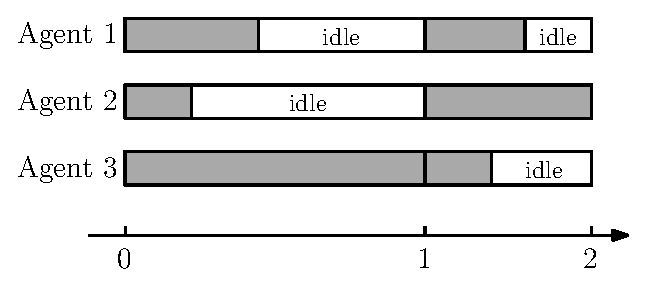
\includegraphics[width=60mm]{./figs/syn-simple}
        \caption{sync-parallel computing}
        \label{fig:parallel_a}
    \end{subfigure} %
    \quad
    \begin{subfigure}[b]{0.45\linewidth}
        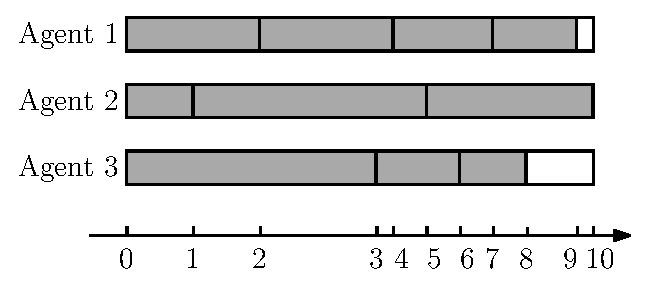
\includegraphics[width=60mm]{./figs/asyn-simple}
        \caption{async-parallel computing}
        \label{fig:parallel_b}
    \end{subfigure} %
    \caption{ Sync-parallel computing (left) versus async-parallel computing (right). On the left, all the agents must wait at idle (white boxes) until the slowest agent has finished.}
    \label{fig:comp_sync_async}
\end{figure}

% \begin{center}[picture: sync-parallel vs async-parallel]\end{center}

Synchronization across all agents means that all agents will wait for  the last (slowest) agent to complete. %It is not truly scalable since, as the number of agents increase, the slowest update  becomes slower and also because it is not fault tolerant. In addition, in the synchronous algorithm, all the processors simultaneously make congestion-inducing communication and memory-access requests.
Async-parallel updates eliminate such idle time, spread out memory access and  communication, and thus often run much faster.  However, async-parallel is more difficult to analyze because of the asynchronous delay.

%Asynchronous delay occurs if, after an agent reads $x$ yet before it completes updating $x_{i_k}$, other agents also make updates to $x$.
%Here, $d_k$ is a scalar in the \emph{consistent} case and a vector in the \emph{atomically inconsistent} case. In the former case, the delays of the entries of $x^{k-d_k}$ are consistent, namely,  $x^{k-d_k}=[x^{k-d_k}_1,\ldots,x^{k-d_k}_n]$. \emph{Atomic inconsistency}, on the other hand, allows inconsistent delays: $x^{k-d_k}=[x^{k-d_{k,1}}_1,\ldots,x^{k-d_{k,n}}_n]$, where $d_k\in\NN^n$ is a vector and $n$ is the number of block coordinates. Inconsistency occurs when multiple agents read and write the entries of $x$ simultaneously, but  atomicity of $x_i$ ensures that all the sub-entries or bits of  $x_i$ are read and written at once and thus stay consistent.

\remove{The sync-parallel update is a special case of the async-parallel update where the number of agents equals $|\II_k|$ and  the asynchronous delay is uniformly zero.}

\textbf{Parallel-update literature.}
Async-parallel methods can be traced back to~\cite{chazan1969chaotic} for systems of linear equations. For function minimization,~\cite{bertsekas1989parallel} introduced an async-parallel gradient projection method. Convergence rates are obtained in~\cite{tseng1991rate-asyn}.
Recently, \cite{bradley2011parallel,richtarik2012parallel} developed parallel randomized methods.

For fixed-point problems, async-parallel methods date back to~\cite{Baudet_1978_asynchronous} in 1978. In  the pre-2010 methods \cite{BMR1997asyn-multisplit,bertsekas1983distributed,Baz200591,el1998flexible} and the review~\cite{Frommer2000201}, each agent updates its own subset of coordinates. Convergence is established under the \emph{$P$-contraction} condition and its variants~\cite{bertsekas1983distributed}. Papers~\cite{Baz200591,Baz1998429} show convergence for async-parallel iterations with simultaneous reading and writing to the same set of components. Unbounded but stochastic delays are considered in~\cite{Strikwerda2002125}.

Recently, random coordinate selection appeared in~\cite{Patrick_2015} for fixed-point problems. The works \cite{nedic2001distributed,recht2011hogwild,liu2013asynchronous,liu2014asynchronous,hsieh2015passcode} introduced async-parallel stochastic methods for function minimization.
For fixed-point problems,~\cite{Peng_2015_AROCK} introduced  async-parallel stochastic methods, as well as several applications.

\subsection{Contributions of This Paper}
The paper systematically discusses the CF properties found in both single and composite operators underlying many interesting applications. We introduce approaches to recognize CF operators and develop coordinate-update algorithms based on them.
We provide a variety of applications to illustrate our approaches.
In particular, we obtain new coordinate-update algorithms for image deblurring, portfolio optimization, second-order cone programming, as well as matrix decomposition. Our analysis also provides guidance to the implementation of coordinate-update algorithms by specifying how to compute certain operators and maintain certain quantities in memory. We also provide numerical results to illustrate the efficiency of the proposed coordinate update algorithms.

This paper does \emph{not} focus on the convergence perspective of coordinate update algorithms, though a convergence proof is provided in the appendix for a new primal-dual coordinate update algorithm. In general, in fixed-point algorithms, the iterate convergence is ensured by the monotonic decrease of the distance between the iterates and the solution set, while in minimization problems, the objective value convergence is ensured by the monotonic decrease of a certain energy function. The reader is referred to the existing literature for details.

%{\color{red}In general, their convergence are ensured by a certain monotonically decreasing energy function in unconstrained minimization, giving  objective value convergence, and by the  monotonically decreasing distance to the solution set in fixed-point problems, giving point convergence (and objective value convergence if applied to minimization). }

%In our fixed-point setting, the operator $\cT$ generally needs to be  nonexpansive (under a certain metric). The operator splitting methods reviewed in~\S\ref{sec:comp-cuf} below generate nonexpansive operators $\cT$ for many problems considered in this paper. The convergence of the resulting stochastic sequential and  (async)-parallel coordinate-update algorithms, as well as their step size selections, is referred to the recent works~\cite{Patrick_2015,Peng_2015_AROCK}. On the other hand,
The structural properties of operators discussed in this paper are irrelevant to  the convergence-related properties such as nonexpansiveness (for an operator) or convexity (for a set or function). Hence, the algorithms developed can be still applied to nonconvex problems.


%\end{subsection}

%\end{section}
% at solving large-sized problems involving  linear and nonlinear maps, and smooth and nonsmooth functions.  at solving large-sized problems involving  linear and nonlinear maps, and smooth and nonsmooth functions.
 %DIF < \DIFdelbegin \DIFdel{It handles both  linear and nonlinear maps, and smooth and nonsmooth functions. The most common examples  }\DIFdelend %DIF > It handles both  linear and nonlinear maps, and smooth and nonsmooth functions. The most common examples


% !TEX root = ./amsa_main.tex
\section{Coordinate Friendly Operators}\label{sec:cuf}

\subsection{Notation}
For convenience, we do not distinguish \emph{a coordinate} from \emph{a block of coordinates} throughout this paper. A coordinate is treated as the unit of variables that are updated together each time. We assume that there are $m$ coordinates and their spaces are $\HH_1,\ldots,\HH_m$. For simplicity, we assume that they are finite-dimensional real Hilbert spaces, though most results hold for general Hilbert spaces. For brevity, we also let $$x = (x_1, \ldots, x_m) \in\HH := \HH_1 \times \cdots \times \HH_m\quad\mbox{and}\quad x_i\in\HH_i,~ i=1,\ldots,m.$$
A function maps from $\HH$ to $\RR$, and an operator maps from $\HH$ to $\GG$, where the definition of $\GG$ depends on the context. The operator $\cT$ and those operators in the splitting methods in \S\ref{sec:splitting} map from $\HH$ to $\HH$.

Several definitions below  use $x,x^+\in\HH$ that \emph{differ by one coordinate}: for some $i\in\{1,\ldots,m\}$ and $\delta_i\in\HH$ that is supported on $\HH_i$,
\beq\label{singleupdate}
x^+ = x+\delta_i.
\eeq
Note that $x^+_j=x_j$ for all $j\not=i$. 

\begin{definition}[number of operations]
We let $\nops{a}{b}$ denote \emph{the number of basic operations} that it takes to compute the quantity $b$ from the  input $a$.
\end{definition}
For example, $\nops{x}{(\cT x)_i}$ denotes the number of operations to compute the $i$th component of $\cT x$ given a general point $x$. We explore the possibility to compute  $(\cT x)_i$ with much fewer operations than what is needed to first compute $\cT x$ and  then take its $i$th component. %Obviously, this number  depends on the structure of $\cT$.   

For a given matrix $A$, let $A_{i,:}$ and $A_{:,j}$ be its $i$th row and $j$th column, respectively. Let $A^\top$ be the transpose of $A$ and $A^\top_{i,:}$ be $(A^\top)_{i,:}$, i.e., the $i$th row of the transpose of $A$. 

\subsection{Single Coordinate Friendly Operators}
This subsection studies a few kinds of CF operators and then formally define the CF operator. We motivate the first kind through an example.
\begin{example}[least squares]\label{ex:lsq1}
We consider the least squares problem
\begin{equation}
\Min_{x} f(x):=\frac{1}{2} \|A x - b\|^2,\label{lsq}
\end{equation}
where $A \in \RR^{p \times m}$ and $b \in \RR^p$. In this example, assume that $m=\Theta(p)$, namely, $m$ and $p$ are of the same order.  We compare the full update of gradient descent and its coordinate update for problem~$\eqref{lsq}$.\footnote{Although gradient descent is seldom used to solve least squares, it often appears as a part in first-order algorithms for problems involving a least squares term.} 
The full update is
$x^{k+1}= \cT x^k $ where
\begin{equation}
\cT x:=x-\eta\nabla f(x)=x-\eta A^\top Ax + \eta A^\top b.
\end{equation}
Assuming that $ A^\top A$ and $ A^\top b$ are made available by pre-computing, we have $\nops{x}{\cT x}=O(m^2)$. The coordinate update at the $k$th iteration performs
$$x_{i_k}^{k+1}=\cT_{i_k} x^k =x^k_{i_k}-\eta\nabla_{i_k} f(x^k),$$
and $x_j^{k+1}=x_j^{k},\forall j\neq i_k$, where $i_k$ is some selected coordinate. 

Since for all $i$, $\left(A^\top (Ax-b)\right)_{i}=(A^\top A)_{i,:}\cdot x-(A^\top b)_{i}$,
we have $\nops{x}{\cT_i x }=O(m)=O(\frac{1}{m}\nops{x}{\cT x})$. Therefore, the coordinate gradient descent is computationally worthy. 
\end{example}
The operator $\cT$ in the above example is a special \emph{Type-I CF} operator.
\begin{definition}[Type-I CF]
For an operator $\cT: \HH\to\HH$, let $\nops{x}{(\cT x)_i}$ be the number of operations for computing the $i$th coordinate of $\cT x$ given $x$ and $\nops{x}{\cT x}$ the number of operations for computing $\cT x$ given $x$. 

We say $\cT$ is \emph{Type-I CF} (denoted as $\cF_1$) if for any $x\in\HH$ and $\forall\, i\in\{1,\ldots,m\}$, it holds
$$\nops{x}{(\cT x)_i}= O\bigg(\frac{1}{m}\nops{x}{\cT x}\bigg).$$
\end{definition}
\begin{example}[least squares II]\label{ex:lsq2}
We can implement the coordinate update in Example \ref{ex:lsq1} in a different manner by maintaining the result $\cT x^k$ throughout, which works when $m=\Theta(n)$ or $p\gg m$. The full update is unchanged. 
At each iteration, we  immediately obtain $x_{i_k}^{k+1}=(\cT x^k )_{i_k}$ but  need to refresh $\cT x^k$ to $\cT x^{k+1}$.
Since $x^{k+1}$ and $x^k$ only differ by just one coordinate, the refreshing only requires multiplying the $i_k$th column of $A^\top A$ by $x^{k+1}_{i_k}-x^k_{i_k}$, which is much cheaper than multiplying $A^\top A$ by $x^{k+1}$. The refreshing takes $O(m)$ operations, which is $O(\frac{1}{m}\nops{x}{\cT (x)})$.
Therefore,
$$\nops{\{ x^k,\cT x^k, x^{k+1}\}}{ \cT x^{k+1}}= O\bigg(\frac{1}{m}\DIFdelbegin  \nops{x^{k+1}}{\cT  x^{k+1}} \bigg).$$
\end{example}
The operator $\cT$ in the above example is a special \emph{Type-II CF} operator.

\begin{definition}[Type-II CF]
An operator $\cT$ is called \emph{Type-II CF} (denoted as $\cF_2$) if, for any $x,i,\delta_i,x^+$ satisfying \eqref{singleupdate}, the following holds
\begin{equation}\label{op-cuf2} \nops{\{ x,\cT x, x^+\}}{ \cT x^+}= O\bigg(\frac{1}{m}\nops{x^+}{\cT x^+}\bigg).
\end{equation}
\end{definition}
Sometimes, maintaining certain quantities other than $\cT x$ can also make the coordinate update computationally worthy.
\begin{example}[least squares III]\label{ex:lsq3}
For the case $p\ll m$, i.e., the system $Ax=b$ is highly underdetermined, we should avoid pre-computing $A^\top A$ because multiplying $A$ and then $A^\top$ is cheaper. Therefore, we change the implementations of both the full and coordinate updates in Example \ref{ex:lsq1}. In particular, the full update
$$x^{k+1}=\cT x^k =x^k-\eta\nabla f(x^k)=x^k-\eta A^\top (Ax^k-b),$$
pre-multiplies $x^k$ by $A$ and then $A^\top$. Hence, 
$\nops{x^k}{\cT(x^k)}=O(mp)$.

We change the coordinate update to maintain the intermediate quantity $Ax^k$. The coordinate update computes 
$$(\cT x^k)_{i_k}=x^k_{i_k}-\eta (A^\top Ax^k-A^\top b)_{i_k},$$
by pre-multiplying $Ax^k$ by $A^{\top}_{i_k,:}$ and refreshing $Ax^k$ to $Ax^{k+1}$ by adding $(x^{k+1}_{i_k}-x^k_{i_k}) A_{:,i_k}$ to $A x^k$. Both steps take $O(p)$ operations, so
\begin{displaymath}{\nops{\{x^k,Ax^k\}}{\{x^{k+1},Ax^{k+1}\}}=O(p)=O\left(\frac{1}{m}\nops{x^k}{\cT x^k}\right)}.\end{displaymath}
\end{example}
Combining Type-I and Type-II CF operators with the last example, we arrive at the following definition:

\begin{definition}[CF operator]
 We say that an operator $\cT:\HH\to\HH$ is \emph{CF} if, for any $x,i,\delta_i,x^+$ satisfying \eqref{singleupdate}, the following holds 
%given any $x\in\HH$ and an arbitrary $i\in\{1,\ldots,m\}$, the coordinate update from $x$ to $x^+$ where $x^+_i = (\cT x)_i$ and $x_{j}^+=x_{j}$ for $j\not=i$, satisfies
\begin{equation}\label{op-cuf} \nops{\{x,\cM(x)\}}{\{x^+,\cM(x^+)\}}= O\bigg(\frac{1}{m}\nops{x}{\cT x}\bigg),
\end{equation}
where $\cM(x)$ is some quantity, possibly non-existing, that is maintained in the memory  to facilitate each coordinate update and refreshed to $\cM(x^+)$. 
\end{definition}

\cut{\begin{definition}[CF operator]
We say that an operator $\cT:\HH\to\GG$ is \emph{coordinate-update (CU) friendly} if for a generic $\eta\in \HH$, $\forall i\in\{1,\ldots,\dim\GG\}$ and $\forall j\in\{1,\ldots,\dim\HH\}$:
\begin{equation}\label{op-cuf}\nops{\{x, \eta_j, \cT x\} }{(\cT (x+\eta_j e_j))_i}\le O\bigg(\frac{1}{\dim \GG}\nops{\{x,\eta,\cT x\}}{\cT (x+\eta)}\bigg).
\end{equation}
(Maintaining quantities other than $x$ and $\cT x$ in  memory is allowed.)
The \emph{set} of CF operators is denoted by  $\cF$. \commzp{$e_j$ is not defined.}
\end{definition}
}

The left-hand side of \eqref{op-cuf} measures the cost of performing one coordinate update (including the cost of updating $\cM(x)$ to $\cM(x^+)$)  while the right-hand side measures the average per-coordinate cost of updating all the coordinates together. When~\eqref{op-cuf} holds, $\cT$ is amenable to coordinate updates.

\cut{\begin{example}Consider for $a,x\in\RR^m$, $$f(x):=\frac{1}{2}\big(\max(0,1-\beta a^\top x)\big)^2,$$ which is the squared hinge loss function. Consider the operator 
\beq\label{qhlossT}
\cT x:=\nabla f(x)=-\beta \max(0,1-\beta a^\top x) a.
\eeq
Let us maintain $\cM(x)=a^\top x$. For arbitrary $x$ and $i$,  let $$x^+_i:=(\cT x)_i=-\beta \max(0,1-\beta a^\top x) a_i$$ and $x^+_j:=x_j,\,\forall j\neq i$. Then, computing $x^+_i$ from $x$ and $a^\top x$ takes $O(1)$ (as $a^\top x$ is maintained), and computing $a^\top x^+$ from $x^+_i-x_i$ and $a^\top x$ costs $O(1)$. Formally, we have
\begin{align*}
&\nops{\{x,a^\top x\}}{\{x^+,a^\top x^+\}}\\
=&\nops{\{x,a^\top x\}}{x^+}+\nops{\{a^\top x,x^+_i-x_i\}}{a^\top x^+}\\
=&O(1)+O(1)=O(1).
\end{align*} 
On the other hand, $\nops{x}{\cT x}=O(m)$. Therefore,~the inequality \eqref{op-cuf} holds, and $\cT$ defined in~\eqref{qhlossT} is CF.
\end{example}
}
\cut{Next, we specify two sub-types of CF operators. They have  stronger properties that are useful when composing with other operators.
\begin{definition} Consider an operator $\cT: \HH\to\HH$.
\begin{itemize}
Let $\mathfrak{M}(x\to (\cT x)_i)$ be the number of operations of computing the $i$-th coordinate of $\cT x$ given $x$ and $\mathfrak{M}(x\to\cT x)$ the number for computing $\cT x$ given $x$.

\item $\cT$ is \emph{Type-I CF} (denoted as $\cF_1$) if for any $x\in\HH$ and $\forall\, i\in\{1,\ldots,m\}$, it holds
$$\nops{x}{(\cT x)_i}= O\bigg(\frac{1}{m}\nops{x}{\cT x}\bigg).$$

%\item Type-II CF ($\cF_2$): an operator $\cT:\HH\to\GG$ is in $\cF_2$ if, for any $x\in\HH$,  $c\in\RR$, it holds that, $\forall i=1,\ldots,\dim\GG$ and $\forall j=1,\ldots,\dim\HH$:  $$\nops{\{x,\cT x,c\}}{(\cT (x+c e_j))_i}\le O\left(\frac{1}{\dim\GG}\nops{\{x,\cT x,c\}}{\cT (x+ce_j)}\right).$$

\item $\cT$ is \emph{Type-II CF} (denoted as $\cF_2$) if, for any $x,i,\delta_i,x^+$ satisfying \eqref{singleupdate}, the following holds: 
\begin{equation}\label{op-cuf2} \nops{\{ x,\cT x, x^+\}}{\cT x^+}= O\bigg(\frac{1}{m}\nops{x^+}{\cT x^+}\bigg)
\end{equation}

\end{itemize}
\end{definition}}
%\begin{remark}
By definition, a Type-I CF operator $\cT$ is CF without maintaining any quantity, i.e., $\cM(x)=\emptyset$. 

A Type-II CF operator $\cT$ satisfies \eqref{op-cuf} with $\cM(x)= \cT x$, so it is also CF. Indeed, given any $x$ and $i$, we can compute $x^+$ by immediately letting $x^+_i=(\cT x)_i$ (at $O(1)$ cost) and keeping $x^+_{j}=x_{j},\,\forall j\neq i$; then, by \eqref{op-cuf2}, we update $\cT x$ to $\cT x^+$ at a low cost. Formally, letting $\cM(x)= \cT x$, %Assume $x$ is updated from $x^-$ and they differ only at the $j$th coordinate, i.e., $x_j=(\cT x^-)_j$ and $x_{j'}=x^-_{j'},\,\forall j'\neq j$. Then we have
\begin{align*}
&\nops{\{x, \cM(x)\}}{\{x^+,\cM(x^+)\}}\\
\le &\nops{\{x, \cT x\}}{x^+} + \nops{\{x, \cT x, x^+\}}{\cT x^+}\\
\overset{\eqref{op-cuf2}}= & O(1) +O\bigg(\frac{1}{m}\nops{x^+}{\cT x^+}\bigg)\\
= & O\bigg(\frac{1}{m}\nops{x}{\cT x}\bigg).
\end{align*} %Type-I CF operators include all separable operators (see Definition \ref{def:sep-op} and Examples \ref{exp:diagmat} through \ref{exp:proj-box} below), and Type-II CF operators include the affine mapping $\cT x=Ax+b$ as a special case.

\cut{\begin{example}[Matrix-vector multiplication]\label{ex:mtx}
Let $A \in \RR^{m \times m}$ be dense, and $A_{i,:},A_{:,i}$ be the $i$th row and the $i$th column of $A$, respectively. Let $b\in\RR^{m}$. Consider $$\cT x:= A x + b,$$ 
and   $x,i,\delta_i,x^+$ satisfying \eqref{singleupdate} for $\HH=\RR^m$. Clearly, $\nops{x}{\cT x}=O(m^2)$.

\begin{enumerate}
\item Since $(\cT x)_i=A_{i,:} x+b_i$ takes $(m+1)$ operations, we have $\nops{x}{(\cT x)_i}=m+1=O(\frac{1}{m}\nops{x}{\cT x})$, so $\cT$ is Type-I CF.
\item Let us maintain $\cM(x)=\cT x$. Since $\cT x^+=\cT x+(x^+_i-x_i)A_{:,i} $ takes $2m+1$ operations, we have $\nops{\{ x,\cT x, x^+\}}{\cT x^+}=O(\frac{1}{m}\nops{x}{\cT x})$. Therefore, $\cT$ is  Type-II CU friendly (by maintaining $\cT x$).
\end{enumerate}
Whether maintaining $\cT x$ or nor will  make significant difference when $\cT$ pre-composes or post-composes another operator.
\end{example}
}
\cut{ let $a_i$ be the $i$th row of $A$. We have $\nops{x}{\cT(x)}=\nops{x}{Ax+b}=m^2+m$, and  $\nops{x}{(\cT }$}
\DIFdelbegin %DIFDELCMD < 

%DIFDELCMD < %%%
In general, the set of CF operators is much larger than the union of Type-I and Type-II CF operators.
%\end{remark}
%{\color{red} we have to declare what one coordinate means here (it can be one block of coordinate whenever it is used together}

%CF operators, as the name suggests, let one compute coordinate updates at little overhead.
Another important subclass of CF operators are operators $\cT:\HH\to\HH$ where   $(\cT x)_i$ only depends on one, or a few, entries out of $x_1,\ldots,x_m$.\cut{, obviously $(\cT x)_i$ is relatively easy to compute. Therefore, they belong to $\cF$.} Based on how many input coordinates they depend on, we partition them into three subclasses.
 \DIFdelbegin %DIFDELCMD < 

%DIFDELCMD < %%%
\DIFdelend \begin{definition}[Separable operator]\label{def:sep-op} Consider $\mathfrak{T}:=\{\cT:\HH\to\HH\}$. We have the partition $\mathfrak{T}=\cC_1\cup\cC_2\cup\cC_3$, where
\cut{We divide the operators into three categories base on the dependency of other coordinates when updating one coordinate.}
\begin{itemize}
\item \emph{separable operators:} $\cT\in\cC_1$ if, for any index $i$, there exists $\cT_i: \HH_i \rightarrow \HH_i$ such that $(\cT x)_i = \cT_i x_i$, that is,   $(\cT x)_i$ only depends on $x_i$.
\item \emph{nearly-separable operators:} $\cT\in \cC_2$ if, for any index $i$, there exists $\cT_i$ and index set $I_i$ such that $(\cT x)_i = \cT_i(\{x_j\}_{j\in I_i})$ with $|I_i| \ll m$, that is, each $(\cT x)_i$ depends on a few  coordinates of $x$.
\item \emph{non-separable operators:} $\cC_3:=\mathfrak{T}\setminus(\cC_1\cup \cC_2)$. If $\cT\in\cC_3$, there exists some  $i$ such that $(\cT x)_i$ depends on many coordinates of $x$.
\end{itemize}
\end{definition}

\cut{For operators in $\cC_1$, the evaluation of $(\cT x)_i$ only involves coordinates $x_i$ and small operator $\cT_i$.  Thus, all the coordinates and the $\cT_i$s are independent with each other, and this is ideal case for coordinate update. For operators in $\cC_2$, the evaluation of $(\cT x)_i$ needs knowledge of some components of $x$.}

Throughout the paper, we assume the coordinate update of a (nearly-) separable operator costs roughly the same for all coordinates. Under this assumption, separable operators are both Type-I CF and Type-II CF, and nearly-separable operators are Type-I CF.\footnote{\label{note1}Not all nearly-separable operators are Type-II CF. Indeed, consider a sparse matrix $A\in \RR^{m\times m}$ whose  non-zero entries are only located  in the last column. Let $\cT x=Ax$ and $x^+=x+\delta_m$. As $x^+$ and $x$ differ by the last entry, $\cT x^+=\cT x+(x^+_m-x_m)A_{:,m}$ takes $m$ operations. Therefore, we have $\nops{\{x,\cT x,x^+\}}{\cT  x^+}=O(m)$. Since $\cT x^+=x^+_mA_{:,m}$ takes $m$ operations, we also have $\nops{x^+}{\cT x^+}=O(m)$. Therefore,~\eqref{op-cuf2} is violated, and there is no benefit  from maintaining $\cT x$.}  %DIF > There are non-separable  CF operators, e.g., Example \ref{ex:lsq1}, \ref{ex:lsq2}, \ref{ex:lsq3}. 
%For example, with a (dense) matrix $A\in\RR^{m\times m}$ and vector $b\in\RR^{m}$, the operator $\cT:x\mapsto A x+b$ is non-separable yet CF. Indeed, let $a_i$ be the $i$th row of $A$. We have $\nops{x}{\cT(x)}=\nops{x}{Ax+b}=m^2+m$, and  $\nops{x}{(\cT x)_i}=\nops{x}{a_i^\top x+b_i}=m+1$, which is much smaller. 

\cut{There are CF operators that are not Type-I . For example, let $f(x)=\sum_{i=1}^m \log [1+\exp(-b_i a_i^\top x)]$. The gradient operator $\nabla f$ is not Type-I CF, but it is CF by caching $a_i^\top x,\, \forall i$.}


\cut{Next, we defined \emph{easy-to-update} operators. While they are not CF,  $\cT x$ can  be easily updated after the input $x$ is changed on one or a few of its coordinates. Therefore, by maintaining $\cT x$  in memory, they are also amenable to coordinate update computing. %For an update-to-update operator $\cT$, \cut{because $\cT x$ can be cheaply updated, }it is important to maintain  $\cT x$  in memory.

\begin{definition}[Easy-to-update]
We say an operator $\cT:\HH\to\GG$ is  \emph{easy-to-update} if, for any $x\in \HH$ and  $c\in\RR$, it holds that $\forall i=1,\ldots,\dim\HH$: $$\nops{\{x,\cT x, c\}}{\cT(x+c e_i)}\le O\left(\frac{1}{\dim\HH}\big(\nops{\{x, c\}}{x+c e_i} +\nops{x+c e_i}{\cT (x+c e_i)}\big)\right).$$
The \emph{set} of {easy-to-update} operators is denoted by $\cE$.
\end{definition}

\cut{A (nearly-) separable operator $\cT$ (i.e., in $\cC_1\cup\cC_2$) is easy-to-coordinate-update if $\cT x$ is maintained in the memory. }


In coordinate-update algorithms, easy-to-update operators \emph{can be treated as} a subclass of CF operators. Seemingly, an easy-to-update operator is not CF since it is not necessarily cheaper to compute $(\cT x)_i$ than the entire $\cT  x$. However, computing the entire $\cT  x$ and changing the entire $x$ add a significantly higher cost to \emph{the next iteration} than computing just $(\cT x)_i$, changing just $x_i$, and taking advantage of the easy-to-update property.
}

%Summarizing this subsection, coordinate update algorithms shall apply CF operators, which include separable, nearly-separable,  linear, as well as easy-to-update operators. 
\cut{
Finally, we define \emph{cheap} and \emph{easy-to-maintain} operators from $\HH$ to $\GG$ that arise in operator compositions.
\begin{definition}[Cheap operator] In an operator composition $\cT=\cT_1 \circ\cdots \circ \cT_p$, an operator $\cT_i:\HH\to\GG$ is cheap if $\nops{x}{\cT_i x}$ is less than or equal to the number of remaining coordinate-update operations, in order of magnitude.
\end{definition}
\begin{definition}[Easy-to-maintain operator]
%If $\cT$ maps from $\HH$ to a different space $\GG$ and it satisfies \eqref{op-cuf2}, we call it 
In an operator composition $\cT=\cT_1 \circ\cdots \circ \cT_p$, an operator $\cT_i:\HH\to\GG$ is \emph{easy-to-maintain} if, for any $x,i,\delta_i,x^+$ satisfying \eqref{singleupdate}, $\nops{\{ x,\cT x, x^+\}}{\cT x^+}$ is less than or equal to the number of remaining coordinate-update operations, in order of magnitude, \emph{or} belongs to $O(\frac{1}{\dim \GG}\nops{x^+}{\cT x^+})$.

The set of  easy-to-maintain operators is denoted by $\cE$. %We call an operator $\cT: \HH\to\GG$ \emph{easy-to-update} if it  and denote the set of these operators as $\cE$.  
\end{definition}
%Easy-to-update operators are used in maintaining quantities.
}

\cut{
\begin{definition}[Easy-to-update]
We say an operator $\cT:\HH\to\GG$ is  \emph{easy-to-update} if, for any $x$ and  $\delta=\sum_{i\in\II}\eta_i e_i$ of arbitrary coefficient $\eta_i\in\RR$ and a small index set $\II$ ($|\II|\ll m$), it holds that  $$\nops{\{x,\cT x,(\eta_i)_{i\in\II}\}}{\cT(\tilde x)}\ll\nops{\{x,(\eta_i)_{i\in\II}\}}{\tilde x} +\nops{\tilde x}{\cT\tilde x},$$
where $\tilde x=x+\delta$. The \emph{set} of {easy-to-update} operators is denoted by $\cE$.
\end{definition}
}

 \cut{When one or a few coordinates of $x$ are changed, giving the new point $\tilde x$, we compute $(\cT \tilde x)_i$ by refreshing $\cT x$ at a low cost. It would be much more expensive to first form $\tilde x$ and then compute $T\tilde x$.}
%In this section, we would like to introduce some properties for single operators.

%
%\begin{definition}[CF]
%One operator is called CF if there is no additional cost for updating all the coordinates one by one independently comparing to updating all the coordinates together. There are mainly three types of CF operators:
%\begin{itemize}
%\item $\cC_1$: updating one coordinate depends ONLY on this coordinate.
%\item $\cC_2$: updating one coordinate depends on SOME coordinates.
%\item $\cC_3$: updating one coordinate depends on ALL coordinates.
%\end{itemize}
%\end{definition}
%\begin{remark}
%We do not consider the cache of computing here. When we consider the derivative of $f(x)$, we consider the each component to be totally unrelated.
%\end{remark}
%\begin{definition}[Block CF]
%One operator is called Block CF if there is no addition cost for updating all the blocks of coordinates one by one independently comparing to updating all the coordinates together. There are mainly three types of Block CF maps:
%\begin{itemize}
%\item $\cB_1$: updating one block of coordinates depends ONLY on this block of coordinates.
%\item $\cB_2$: updating one block of coordinates depends on SOME blocks of coordinates.
%\item $\cB_3$: updating one block of coordinates depends on ALL blocks of coordinates.
%\end{itemize}
%\end{definition}
%\begin{remark}Note that Block CF is just a block version of CF. For Block CF operators, updating all the coordinates one by one independently may introduce additional cost comparing to updating all the coordinates.
%\end{remark}

%To illustrate the properties, we introduce several examples for all the cases.
%\subsection{BC-friendly with property $\cC_1$}
%Assume $\HH = \HH_1 \times \cdots \times \HH_m$, where $m > 0 $ is the number of coordinates. If $\cT: \HH \rightarrow \HH$ satisfies the following
%\begin{align}
%(\cT x)_i = \cT_ix_i, \quad i=1,\cdots,m
%\end{align}
%%$$\cT = \begin{bmatrix}\cT_1 & & \\ & \ddots& \\ & & \cT_m\end{bmatrix},$$
%where $\cT_i: \HH_i \rightarrow \HH_i$, then $\cT$ is CF with $\cC_1$. We denote $\cT$ as $\cT=\cT_{1}\times\cdots\times \cT_{m}$. Thus, computing $\cU_i \circ \cT x$ takes no extra effort, since
%$$(\cU_i \circ \cT) x = (\cT x)_i = \cT_i x_i.$$
%The computation only involves a coordinates $x_i$ and a small operator $\cT_i$.  It would be embarrassingly parallelization, since the coordinates and the $\cT_i$s are independent with each other, and the computation can be carried out without any communication.
\subsection{Examples of CF Operators}\label{sec:exp-cuf}
In this subsection, we give  examples of CF operators arising in different areas including linear algebra, optimization, and machine learning.
\begin{example}[(block) diagonal matrix]\label{exp:diagmat}
Consider the diagonal matrix
$$A = \begin{bmatrix}a_{1,1} & ~ & 0 \\  & \ddots&  \\ 0& ~& ~a_{m,m}\end{bmatrix}\in\RR^{m\times m}.$$
Clearly $\cT:x\mapsto Ax$ is separable.
\end{example}
\begin{example}[gradient and proximal maps of a separable function]
Consider a \emph{separable} function
$$f(x) = \sum_{i=1}^m f_i(x_i).$$
Then, both $\nabla f$ and $\prox_{\gamma f}$ are separable, in particular,
$$(\nabla f(x))_i = \nabla f_i (x_i) \quad \mbox{and}\quad (\prox_{\gamma f}(x))_i= \prox_{\gamma f_i} (x_i).$$\cut{$$\nabla f(x) = \begin{bmatrix} \nabla f_1 (x_1) \\ \vdots \\ \nabla f_m(x_m) \end{bmatrix} \quad \mbox{and}\quad \prox_{\gamma f}(x) = \begin{bmatrix}  \prox_{\gamma f_1} (x_1) \\ \vdots \\  \prox_{\gamma f_m}(x_m) \end{bmatrix}.$$}
Here, $\prox_{\gamma f} (x)$ ( $\gamma >0$) is the \emph{proximal operator} that we  define in \eqref{def-prox}. %returns the minimizer $y^*$ of the function $f(x) + \frac{1}{2\gamma } \|x - y\|^2$. The minimizer exists and is unique when $f$ is a closed proper convex function.
% $$\prox_{\gamma f} (x): = \argmin_{y \in \HH} f(x) + \frac{1}{2\gamma } \|x - y\|^2,$$
% for which we assume unique minimizer (true if $f$ is closed proper convex).
\end{example}

\begin{example}[projection to box constraints]\label{exp:proj-box}
%\commwy{Please move this example to below $\cC_1$. Use the box constraint example instead of $\ell_\infty$ ball since the latter is a special example. Also, please add a proposition that $\cC_1\cup\cC_2\subset\cE$, which is obvious.}
Consider the ``box" set $B:=\{x:a_i\leq x_i\leq b_i,~i=1,\ldots,m\}\subset\RR^m$. Then, the projection operator $\prj_{B}$ is separable. Indeed,
$$\big(\prj_{B}(x)\big)_i=\max(b_i,\,\min(a_i,\, x_i)).$$
%\begin{equation}
%\big(\prj_{B}(x)\big)_i =
%\left\{
%\begin{array}{ll}
%b_i &\text{ if }  x_i \in [b_i, +\infty) \\
%a_i &\text{ if } x_i \in (-\infty, a_i] \\
% x_i &\text{ if } x_i \in [a_i, b_i].
%\end{array}
%\right.
%\end{equation}
\end{example}


\begin{example}[sparse matrices] If every row of the matrix $A\in\RR^{m\times m}$ is sparse,   $\cT :x\mapsto Ax$ is nearly-separable.
%$$A = \begin{bmatrix}A_{11} & A_{12} & \\ A_{21}& A_{22} & \ddots \\ & \ddots & \ddots & A_{m-1,m}\\&  & A_{m,m-1} & A_{m,m}\end{bmatrix},$$
%is a sparse supported map.

Examples of sparse matrices arise from various finite difference schemes for differential equations, problems defined on sparse graphs. When most pairs of a set of random variables  are conditionally independent, their inverse covariance matrix is sparse.
\end{example}

\begin{example}[sum of sparsely supported functions]
Let $E$ be a class of index sets and every $e\in E$ be a small subset of $\{1, ..., m\}$, $|e|\ll m$. In addition $\#\{e:i\in e\}\ll \#\{e\}$ for all $i\in\{1,\ldots,m\}$.
Let $x_e:=(x_i)_{i\in e}$, and  
$$f(x) = \sum_{e \in E} f_e (x_e).$$ 
The gradient map $\nabla f$ is nearly-separable.


An application of this example arises in wireless communication over  a graph of $m$ nodes. Let each $x_i$ be the spectrum assignment to node $i$, each $e$ be a neighborhood of nodes,  and each   $f_e$ be a utility function. The input of $f_e$ is $x_e$ since the utility depends on the spectra assignments in the neighborhood.

In  machine learning, if each observation only involves with a few features, then each function of the optimization objective will depend on a  small number of components of $x$.  \cut{The gradient of $f(x)$ will also only depend on a few coordinates of $x$. \commwy{could you be specific in the machine learning example?}}
\end{example}

\cut{ % have been moved
\begin{example}[matrix-vector multiplication]\label{mtxexam}
With a (dense) matrix $A\in\RR^{m\times m}$, the operator $\cT:x\mapsto A x$ is non-separable yet CF. Indeed, let $a_i$ be the $i$th row of $A$. Then, we can compare $\nops{x}{\cT(x)}=\nops{x}{Ax}=m^2$, and  $\nops{x}{(\cT x)_i}=\nops{x}{a_i^T x}=m$ is much smaller.
%Observe that the complexity of $\cS_i \circ (\cT x)$ is $O(m n)$, however, the complexity for evaluating $\cT x$ is $O(n^2)$. We can choose $m \ll n$, then the affine map $\cT$ is BC-friendly.
%The extra cost we pay for parallelization is that $x$ needs to be read $n/m$ times instead of once compared to the serial implementation.
\end{example}
\begin{example}[affine transformation preserves $\cC_1$]
Let $\cT\in\cC_1$, $b \in \HH$. Then $\cT':x\mapsto\cT x + b$ belongs to  $\cC_1$.
\end{example}
}
\cut{\begin{example}[projection to the Euclidean ball]\label{ex:projball}
Let $B_2=\{x\in\RR^m:\|x\|_2\leq r\}$ and $$\cT x:=\prj_{B_2}(x).$$ By definition, %$\cT(x)=\argmin_y \{\|y-x\|_2:\|y\|_2\le r\}$
%\begin{equation}
$\cT(x) =\xi x,~\mbox{where}~\xi=\min\left\{1,\frac{r}{\|x\|_2}\right\}.$
%\end{equation}
Since $\cT x$ depends on all the entries of $x$,  $\cT$ is non-separable.

Nonetheless, the norm map $\cT':x\mapsto \|x\|_2$ is easy-to-maintain. Indeed, given $x$, we can maintain $\cT'(x)=\|x\|_2$. If $x_i$ is updated,  letting $e_i$ be the $i$th standard basis and writing $\bar{x}=x+\eta e_i$, it follows $\|\bar{x}\|_2=\sqrt{\|x\|_2^2+2\eta x_i+\eta^2}$. Therefore,   $\nops{\{x,\|x\|_2,\eta\}}{\|\bar{x}\|_2}=O(1)$ while $\nops{\bar{x}}{\|\bar{x}\|_2}=O(m)$.

\end{example}
}


%{\color{red}These two examples should be moved back}


\cut{\begin{example}[$\cC_2 + \cC_2= \cC_3$]
Let $A_1,A_2\in\RR^{m\times m}$ be sparse matrices. If $A_1+A_2$ is a dense matrix, then $\cT x= Ax=A_1x+A_2x$ belongs to $\cC_3$ though $\cT_1 x= A_1x$ and $\cT_2=A_2x$ both belong to $\cC_2$.
\end{example}
}


%\begin{example}[Linear combination of maps]
%The linear combination of block separable maps with any other BC-friendly maps is also BC-friendly. For example, $I - \gamma \, \nabla f$ is BC-friendly if $\nabla f$ is BC-friendly.
%\end{example}


%\subsection{BC-friendly with property $\cC_2$}
%\begin{definition}[Sparsely supported map]
%Let $I_i$ be a subset of $\{1, ..., m\}$. Consider $\cT: \HH \rightarrow \HH$ that satisfies
%\begin{equation}
%(\cT x)_i = \cT_i(\{x_j\}_{j\in I_i}).
%\end{equation}
%That is evaluating $(\cT x)_i$ only requires knowledge of those components of $x_j$ for $j \in I_i$. If the maximum cardinality $\max_{i} |I_i| \leq c$ and $c \ll m$, then $\cT$ is said to be \emph{sparsely supported}.
%\end{definition}
%%Since for all $i$, evaluating $(\cT x)_i$ only requires a few coordinates of $x$, hence it is significantly easier than computing $\cT x$. As a consequence, sparsely supported maps are BC-friendly.
%
%
\cut{
Based on the categories of an operator and the examples, we know that all operators in $\cC_1$ are CF, operators in $\cC_2$ with $c\ll m$ is also CF. However, some operator in $\cC_3$ are CF, while others are not. There are other ways to determine whether a combination of several operators is CF or not. }

\cut{\begin{remark}
If the complexity of evaluating $\cT_2 x$ is smaller or equals to the complexity of evaluating $\cT_{1,i} x$, then whether the operators $\cT_1+\cT_2$ and $\cT_1\circ\cT_2$ is CF or not depends on whether $\cT_2$ is CF or not.
\end{remark}}

%{\color{red} If $\cT = \cT_1 \circ \cT_2$, easy-to-update also means the complexity of evaluating $\cT_2 \, x$ is smaller or equals to the complexity of evaluating $\cT_{1, i} \, x$. }


%
%
%\subsection{Easy to compute}
%A function $r$ is \emph{proximal friendly} if the following problem  {\color{blue} is not difficult, (or say has closed form representation.)}
%\begin{equation}
%\prox_r(x) = \argmin_{y} r(y) + \frac{1}{2} \|x - y\|^2.
%\end{equation}
%As we have shown before, if $r(x)$ is block separable, then the $\prox_r$ is also block separable. Examples of such include $\ell_1$ norm, indicate function of box constraints $\{x ~|~ a \leq x \leq b\}$, and the $\ell_{2,1}$ norm. Some other non separable examples but easy to evaluate their proximal map include indicate function of $\ell_2$ ball, $\ell_1$ ball, and indicate function of the probability simplex $\{x~|~ \sum_{i=1}^n x_i = 1, x_i \geq 0\}$. The proximal maps correspond to the projection of the sets.
%


%
%\subsection{Easy-to-update maps}
%[NEED TO REFINE THE DEFINITION] An operator $\cT: \HH \rightarrow \HH$ is easy-to-update, if
%$$O(\cT (x + \sum_{i \in \II} \eta_i e_i )) \ll O (\cT \, y), \forall y$$
%where $|\II| \ll m$.

%{\color{red} If $\cT = \cT_1 \circ \cT_2$, easy-to-update also means the complexity of evaluating $\cT_2 \, x$ is smaller or equals to the complexity of evaluating $\cT_{1, i} \, x$. }

%Following the above example, we define the \emph{easy-to-update} operator, where caching is allowed.

\cut{When we apply coordinate update algorithms, we may choose to store some intermediate variables which are easy to update after some coordinates are updated.}

\cut{
\begin{definition} Let $\mathfrak{M}[x\to \cT(x)]$ denote the number of  operations of computing $\cT(x)$ given $x$. Let $\mathfrak{M}[y\to \tilde y]$ denote the number of  operations of computing $\tilde y$ in place given  $y$.
\end{definition}}

\cut{
\begin{remark}By  definition, a separable operator is easy to update (and no quantity needs to be maintained), but not all nearly-separable operators easy to update. For example, consider a sparse matrix $A\in R^{m\times m}$ where all of its non-zero entries are in the last column. Let $\cT x=Ax$ and, given a point $x$ nd $\tilde x=x+\eta_me_m$, compute $(T(x+\eta_me_m))_m$. We have $\nops{\{x,\cT x,\eta_m\}}{\cT \tilde x}=O(m)$ and $\nops{\{x,\eta_m\}}{\tilde x} +\nops{\tilde x}{\cT(\tilde x)}=O(1)+O(m)=O(m)$. There is not benefit  from maintaining $\cT x$.
\end{remark}
}
\begin{example}[square hinge loss function]\label{ex:qhloss}
Consider for $a,x\in\RR^m$, $$f(x):=\frac{1}{2}\big(\max(0,1-\beta a^\top x)\big)^2,$$ which is the squared hinge loss function. Consider the operator 
\beq\label{qhlossT}
\cT x:=\nabla f(x)=-\beta \max(0,1-\beta a^\top x) a.
\eeq
Let us maintain $\cM(x)=a^\top x$. For arbitrary $x$ and $i$,  let $$x^+_i:=(\cT x)_i=-\beta \max(0,1-\beta a^\top x) a_i$$ and $x^+_j:=x_j,\,\forall j\neq i$. Then, computing $x^+_i$ from $x$ and $a^\top x$ takes $O(1)$ (as $a^\top x$ is maintained), and computing $a^\top x^+$ from $x^+_i-x_i$ and $a^\top x$ costs $O(1)$. Formally, we have
\begin{align*}
&\nops{\{x,a^\top x\}}{\{x^+,a^\top x^+\}}\\
=&\nops{\{x,a^\top x\}}{x^+}+\nops{\{a^\top x,x^+_i-x_i\}}{a^\top x^+}\\
=&O(1)+O(1)=O(1).
\end{align*} 
On the other hand, $\nops{x}{\cT x}=O(m)$. Therefore,~\eqref{op-cuf} holds, and $\cT$ defined in~\eqref{qhlossT} is CF.
\end{example}


\cut{\rev{\subsection{Compare Full Update with Coordinate Update}\label{lsqexperiment}
In this subsection, we compare the efficiency of four different coordinate update schemes (cyclic, cyclic permutation, random, and greedy with Gauss-Southwell rule) with the full gradient descent method for solving the least square problem 
$$\Min_{x} \frac{1}{2} \|A x - b\|^2,$$
where $A \in \RR^{p \times m}$ and $b \in \RR^p$. We solve the above problem with the following update scheme
$$x^{k+1} = x^k - \eta_k A^{\top}(A x^k - b),$$
where $\eta_k$ is the step size. This test uses three datasets, which are summarized in Table \ref{tab:ls-data}.  
\begin{table}[!hbtp]
\centering
 \begin{tabular}{lrrrr}
  \toprule
     & $p$  & $m$ & $A$ & $b$\\
   \midrule
   Dataset I & 1000 & 1000 & \texttt{diag([1:m])} & \texttt{ones(m, 1)} \\
   Dataset II & 1000 & 500 & \texttt{randn(m, n)} & \texttt{ones(m, 1)} \\
   Dataset III & 1000 & 500 & \texttt{rand(m, n)} & \texttt{ones(m, 1)} \\
   \bottomrule
\end{tabular}
 \caption{Three datasets for the least square problem\label{tab:ls-data}}
\end{table}

For both full gradient descent method, the step size $\eta$ is set to $\frac{2}{\|A\|_2^2}$. For the four coordinate update methods, if coordinate $i$ is selected, then $\eta_k$ is set to $\frac{1}{(A^{\top}A)_{ii}}$. Since all of the methods have same per epoch complexity, so we measure and compare the per epoch progress in terms of objective error. Figure \ref{fig:ls_a} shows that for Dataset I, both cyclic update, cyclic permutation, and greedy update converge to the optimal solution with one epoch. Random coordinate update converges to the optimal solution after $8$ epochs. However, due to the small step size ($\eta_k = 10^{-6}$), the gradient descent algorithm converges very slowly. For the other two datasets, we observe that greedy coordinate update converges faster than the other methods, and random coordinate update and cyclic shuffle coordinate update give consistent better performance than the full gradient descent algorithm. 
\begin{figure}[!htbp] \centering
    \begin{subfigure}[b]{0.3\linewidth}
        \includegraphics[width=40mm]{./figs/diag_matrix_cropped.pdf}
        \caption{Dataset I}
        \label{fig:ls_a}
    \end{subfigure} %
    \quad
    \begin{subfigure}[b]{0.3\linewidth}
        \includegraphics[width=40mm]{./figs/randn_matrix_cropped.pdf}
        \caption{Dataset II}
        \label{fig:ls_b}
    \end{subfigure} %
    \quad
    \begin{subfigure}[b]{0.3\linewidth}
        \includegraphics[width=40mm]{./figs/rand_matrix_cropped.pdf}
        \caption{Dataset III}
        \label{fig:ls_c}
    \end{subfigure} %
    \caption{Compare the convergence of four different coordinate update algorithms with full gradient descent algorithm.}
    \label{fig:3s_results}
\end{figure}
}
}

\cut{
\begin{example}[scalar map pre-composing affine function]\label{exp:log-grad} Let $a_j\in \RR^m, b_j\in \RR$ and $\phi_j:\RR\to \RR$ be differentiable functions, $j=1,\ldots,p$. Let $$f(x)=\sum_{j=1}^p \phi_j(a_j^\top x +b_j).$$ Assume that evaluating $\phi'_j$ costs $O(1)$ for all $j$. Then, $\nabla f$ is CF (by maintaining $a_j^\top x+b_j,\,\forall j$), but it is neither Type-I nor Type-II CF if $A=[a_1,\ldots,a_p]^\top$ is dense. Indeed, let $$\cT_1 y:=A^\top y,\quad \cT_2 y := \Diag(\phi_1'(y_1),\ldots,\phi_p'(y_p)), \quad \cT_3 x := Ax+b.$$ Then $\nabla f(x)= \cT_1\circ\cT_2\circ\cT_3 x$. For any $x$ and $i\in\{1,\ldots,m\}$, let $x^+_i=\nabla_i f(x)$ and $x^+_j=x_j,\forall j\neq i$, and let $\cM(x)=\cT_3 x$. We can first compute $\cT_2\circ\cT_3 x$ from $\cT_3 x$ for $O(p)$ operations, then compute $\nabla_i f(x)$ and thus $x^+$ from $\{x, \cT_2\circ\cT_3 x\}$ for $O(p)$, and finally update the maintained $\cT_3 x$ to $\cT_3 x^+$ from $\{x, x^+,\cT_3 x\}$ for another $O(p)$. Formally,
\begin{align*}
&\nops{\{x,\cT_3 x\}}{\{x^+, \cT_3x^+\}}\cr
=& \nops{\cT_3x}{\cT_2\circ\cT_3 x}+\nops {\{x,\cT_2\circ\cT_3 x\}}{x^+}+\nops{\{x,\cT_3 x, x^+\}}{\{\cT_3x^+\}}\cr
=& O(p) + O(p) +O(p)=O(p).\nonumber
\end{align*}
On the other hand, $\nops{x}{\nabla f(x)}=O(pm)$. Therefore
$\nabla f= \cT_1\circ\cT_2\circ\cT_3$ is CF. 

Once $p=m$, $\cT_1,\cT_2,\cT_3$ all map from $\RR^m$ to $\RR^m$. Then, it is easy to check that $\cT_1$ is Type-I CF, $\cT_2$ is separable, and $\cT_3$ is Type-II CF. The last one is crucial since not maintaining $\cT_3 x$ would disqualify $\cT$ from CF. Indeed, to obtain $(\cT x)_i$, we must multiple $A_i^\top$ to all the entries of $\cT_2\circ\cT_3 x$, which in turn needs all the entries of $\cT_3 x$, computing which from scratch costs $O(pm)\gg O(p)$.

There are some  rules to preserve Type-I and Type-II CU-friendliness. For example, $\cT_1\circ \cT_2$ is still Type-I CF, and $\cT_2\circ\cT_3$ is still CF but there are counter examples where  $\cT_2\circ\cT_3$  can be neither Type-I or Type-II CF in general. Such properties are important for developing efficient coordinate update algorithms for complicated problems; see the next section.
\end{example}
}


%\input{cu_single_bcf}


% !TEX root = ./amsa_main.tex
\section{Composite Coordinate Friendly Operators}\label{sec:comp-cuf}
Compositions of two or more operators arise in  algorithms for problems that have composite functions, as well as  algorithms that are derived from operator splitting methods. To update the variable update $x^k$ to $x^{k+1}$, two or more operators are sequentially applied, and therefore the structures of all  operators  determine whether the update is CF. This is where CF structures become less trivial but more interesting. This section studies composite CF operators. The exposition leads to the recovery of existing algorithms, as well as powerful new algorithms.

\cut{Operator splitting algorithms decompose awkward combinations of operators into simpler subproblems. They give rise to a lot of efficient algorithms. \rev{Aside from the widely used ADMM and the primal-dual algorithms \cite{chambolle2011first}\cite{condat2013primal}\cite{vu2013splitting}, the forward-backward splitting, the forward-backward-forward splitting, the Douglas-Rachford splitting, the forward-Douglas-Rachford splitting also find numerous applications \cite{daubechies2003iterative}\cite{combettes2005signal}\cite{o2014primal}\cite{briceno2015FDRS} in machine learning, signal processing and imaging. Morover, the development of operator splitting schemes can produce more powerful algorithms \cite{davis2015three}. Combining operator splitting and coordinate updating will give us algorithms enjoying benefits from both sides. However, naively applying coordinate update to existing algorithms may results in divergence or wrong answers.
\begin{example}[three block ADMM]
The problem:
\begin{equation}
\begin{array}{l}
\underset{x,y,z\in\RR^m}{\textnormal{minimize  }} ~f(x)+g(y)+h(z)\\
\textnormal{subject to } Ax+Bx+Cz=b,
\end{array}\label{3block}
\end{equation}
can be solved by the following ADMM iterations:
\begin{equation}
\left\{
\begin{array}{ll}
x^{k+1}&=\argmin_x f(x)+\frac{\eta}{2}\|Ax+By^k+Cz^k+\frac{s^k}{\eta}-b\|^2,\\
\begin{pmatrix}
y^{k+1}\\
z^{k+1}
\end{pmatrix}&=\argmin_{(y,z)^\top }g(y)+h(z)+\frac{\eta}{2}\|Ax^{k+1}+By+Cz+\frac{s^k}{\eta}-b\|^2,\\
s^{k+1}&=s^k+\eta(Ax^{k+1}+By^{k+1}+Cz^{k+1}-b).
\end{array}\right.
\end{equation}
However, if we apply sequential update to the $(y,z)$ subproblem, we will have the following iterative scheme:
\begin{equation}
\left\{
\begin{array}{l}
x^{k+1}=\argmin_x f(x)+\frac{\eta}{2}\|Ax+By^k+Cz^k+\frac{s^k}{\eta}-b\|^2,\\
y^{k+1}=\argmin_y g(y)+\frac{\eta}{2}\|Ax^{k+1}+By+Cz^k+\frac{s^k}{\eta}-b\|^2,\\
z^{k+1}=\argmin_z h(z)+\frac{\eta}{2}\|Ax^{k+1}+By^{k+1}+Cz+\frac{s^k}{\eta}-b\|^2,\\
s^{k+1}=s^k+\eta(Ax^{k+1}+By^{k+1}+Cz^{k+1}-b).
\end{array}\right.
\end{equation}
It is the direct extension of ADMM to three block, which is proved to be divergent in \citep{chen2014direct}
\end{example}}
This motivates us to study the mechanism to develop coordinate update algorithms based on operator splitting. In order to do this, we study when the combinations of operators is CF in  In \S\ref{sc:comb}. Then, in \S\ref{sec:splitting} review several operator splitting schemes and provide examples. \rev{We point out here that the coordinate update methods we propose, based on operator splitting schemes, all have convergence guarantee, at least for async-parallel (thus also stochastic) update \cite{Peng_2015_AROCK}}


There are many popular operator-splitting based algorithms, e.g., proximal gradient method, ADM, and primal-dual method, which reduce the original problem to simpler subproblems, each corresponding to a part of the objective or constraints. Coordinate updates can be combined with operator splitting to further simplify their subproblems and even offer better parallelism. Most operator splitting algorithms are sequential compositions of two or more operators. This section studies when their compositions are CF operators.

}

\subsection{Combinations of Operators}\label{sc:comb}
We start by an example with numerous applications. It is a generalization of Example~\ref{ex:qhloss}.
\begin{example}[scalar map pre-composing affine function]\label{exp:log-grad} Let $a_j\in \RR^m, b_j\in \RR$, and $\phi_j:\RR\to \RR$ be differentiable functions, $j \in [p]$. Let $$f(x)=\sum_{j=1}^p \phi_j(a_j^\top x +b_j).$$ Assume that evaluating $\phi'_j$ costs $O(1)$ for each $j$. Then, $\nabla f$ is CF. Indeed, let $$\cT_1 y:=A^\top y,\quad \cT_2 y := \Diag(\phi_1'(y_1),\ldots,\phi_p'(y_p)), \quad \cT_3 x := Ax+b,$$ 
where $A=[a_1^\top; a_2^\top; \ldots,a_p^\top]\in \RR^{p\times m}$ and $b=[b_1;b_2;\ldots;b_p]\in\RR^{p\times 1}$. Then we have $\nabla f(x)= \cT_1\circ\cT_2\circ\cT_3 x$. For any $x$ and $i\in[m]$, let $x^+_i=\nabla_i f(x)$ and $x^+_j=x_j,\forall j\neq i$, and let $\cM(x):=\cT_3 x$. We can first compute $\cT_2\circ\cT_3 x$ from $\cT_3 x$ for $O(p)$ operations, then compute $\nabla_i f(x)$ and thus $x^+$ from $\{x, \cT_2\circ\cT_3 x\}$ for  $O(p)$ operations, and finally update the maintained $\cT_3 x$ to $\cT_3 x^+$ from $\{x, x^+,\cT_3 x\}$ for another $O(p)$ operations. Formally,
\begin{align*}
&\nops{\{x,\cT_3 x\}}{\{x^+, \cT_3x^+\}}\cr
=& \nops{\cT_3x}{\cT_2\circ\cT_3 x}+\nops {\{x,\cT_2\circ\cT_3 x\}}{x^+}+\nops{\{x,\cT_3 x, x^+\}}{\{\cT_3x^+\}}\cr
=& O(p) + O(p) +O(p)=O(p).\nonumber
\end{align*}
Since $\nops{x}{\nabla f(x)}=O(pm)$, therefore
$\nabla f= \cT_1\circ\cT_2\circ\cT_3$ is CF. 

If $p=m$, $\cT_1,\cT_2,\cT_3$ all map from $\RR^m$ to $\RR^m$. Then, it is easy to check that $\cT_1$ is Type-I CF, $\cT_2$ is separable, and $\cT_3$ is Type-II CF. The last one is crucial since not maintaining $\cT_3 x$ would disqualify $\cT$ from CF. Indeed, to obtain $(\cT x)_i$, we must multiple $A_i^\top$ to all the entries of $\cT_2\circ\cT_3 x$, which in turn needs all the entries of $\cT_3 x$, computing which from scratch would cost $O(pm)$.

There are general rules to preserve Type-I and Type-II CF. For example, $\cT_1\circ \cT_2$ is still Type-I CF, and $\cT_2\circ\cT_3$ is still CF, but there are counter examples where  $\cT_2\circ\cT_3$  can be neither Type-I nor Type-II CF. Such properties are important for developing efficient coordinate update algorithms for complicated problems; we will formalize them in the following.
\end{example}

The operators $\cT_2$ and $\cT_3$ in the above example are prototypes of \emph{cheap} and \emph{easy-to-maintain} operators from $\HH$ to $\GG$ that arise in operator compositions.
\begin{definition}[cheap operator] For a composite operator $\cT=\cT_1 \circ\cdots \circ \cT_p$, an operator $\cT_i:\HH\to\GG$ is cheap if $\nops{x}{\cT_i x}$ is less than or equal to the number of remaining coordinate-update operations, in order of magnitude.
\end{definition}

\begin{definition}[easy-to-maintain operator]
%If $\cT$ maps from $\HH$ to a different space $\GG$ and it satisfies \eqref{op-cuf2}, we call it 
For a composite operator $\cT=\cT_1 \circ\cdots \circ \cT_p$, an operator $\cT_j:\HH\to\GG$ is \emph{easy-to-maintain}, if for any $x,i,\delta_i,x^+$ satisfying \eqref{singleupdate}, $\nops{\{ x,\cT_j x, x^+\}}{\cT_j x^+}$ is less than or equal to the number of remaining coordinate-update operations, in order of magnitude, \emph{or} belongs to $O(\frac{1}{\dim \GG}\nops{x^+}{\cT x^+})$.  
\end{definition}
\cut{\begin{example}[projection to the Euclidean ball]\label{ex:projball}
Let $B_2=\{x\in\RR^m:\|x\|_2\leq r\}$ and $$\cT x:=\prj_{B_2}(x).$$ By definition, %$\cT(x)=\argmin_y \{\|y-x\|_2:\|y\|_2\le r\}$
%\begin{equation}
$\cT(x) =\xi x,~\mbox{where}~\xi=\min\left\{1,\frac{r}{\|x\|_2}\right\}.$
%\end{equation}
Since $\cT x$ depends on all the entries of $x$,  $\cT$ is non-separable.

Nonetheless, the norm map $\cT':x\mapsto \|x\|_2$ is easy-to-maintain. Indeed, given $x$, we can maintain $\cT'(x)=\|x\|_2$. If $x_i$ is updated,  letting $e_i$ be the $i$th standard basis and writing $\bar{x}=x+\eta e_i$, it follows $\|\bar{x}\|_2=\sqrt{\|x\|_2^2+2\eta x_i+\eta^2}$. Therefore,   $\nops{\{x,\|x\|_2,\eta\}}{\|\bar{x}\|_2}=O(1)$ while $\nops{\bar{x}}{\|\bar{x}\|_2}=O(m)$.

\end{example}
}

\cut{\begin{example}[Projection to Euclidean ball]
Let $\cT \, x = \Proj_{\|x\|_2 \leq r} (x)$, $\tilde x  = x + \sum_{i \in \II} \eta_i e_i$
\begin{equation}
\cT \, (\tilde x) =
\left\{
\begin{array}{ll}
\tilde x &\text{ if } \|\tilde x\| \leq r \\
\frac{r}{\|\tilde x\|} \tilde x &\text{ if } \|\tilde x\| > r,
\end{array}
\right.
\end{equation}
Note that $\|\tilde x\|^2 = \|x\|^2 + 2 \sum_{i \in \II} \langle x_i + \eta_i, \eta_i \rangle$. If $ \|\tilde x\| \leq r$, then $\cT$ is easy to update if and only if $ \|\tilde x\| \leq r$.
\end{example}}


The splitting schemes in \S\ref{sec:splitting} below will be based on $\cT_1+\cT_2$ or $\cT_1\circ\cT_2$, as well as a sequence of such combinations. If $\cT_1$ and $\cT_2$ are both CF, $\cT_1+\cT_2$ remains CF, but $\cT_1\circ\cT_2$ is not necessarily so. This subsection discusses how $\cT_1\circ\cT_2$ inherits the properties from $\cT_1$ and $\cT_2$. Our results are summarized in Tables \ref{table:comp1-op} and \ref{table:comp-op} and explained in detail below.

The combination \cut{$\cT_1+\cT_2$ and }$\cT_1\circ \cT_2$ generally inherits the \emph{weaker} property from $\cT_1$ and $\cT_2$. %If one of them is separable and the other nearly-separable, then $\cT_1\circ \cT_2$ is nearly-separable. % since the composition depends on more than one coordinate of $x$.

The separability ($\cC_1$) property  is  preserved by composition. If $\cT_1,\ldots,\cT_n$ are separable, then $\cT_1\circ\cdots\circ \cT_n$ is separable.  However, combining  nearly-separable ($\cC_2$) operators  may not yield a nearly-separable operator since\cut{ Even if  $\cT_1,\ldots,\cT_n\in\cC_2$ and each $(\cT_jx)_i$ depends on $c>1$ coordinates of $x$, the composition $(\cT_1\circ\cdots\circ \cT_n x)_i$ can depend on the much more $\min\{c^n,m\}$ components of $x$, as} composition introduces more dependence among the input entries. Therefore, composition of nearly-separable operators can be either nearly-separable or non-separable.

%\begin{center}\begin{tabular}{|c|c|c|}\hline
%$\cT_1$ & $\cT_2$ & $\cT_1+\cT_2$\\\hline
%$\cC_1$ & $\cC_1$/$\cC_2$/$\cC_3$ & $\cC_1$/$\cC_2$/$\cC_3$\\\hline
%$\cC_2$ & $\cC_2$ & $\cC_2$ or $\cC_3$\\\hline
%$\cC_2$/$\cC_3$ & $\cC_3$ & $\cC_3$\\\hline
%\end{tabular}\end{center}
%\begin{center}\begin{tabular}{c|l|l|l|l}
%Case & $\cT_1\in$ & $\cT_2\in$ & $~(\cT_1+\cT_2) \in~$ & $~(\cT_1\circ\cT_2)\in ~$\\\hline\hline
%1 & $\cC_1$ (separable) & $\cC_1$, $\cC_2$, $\cC_3$ & \multicolumn{2}{|l}{$\cC_1$, $\cC_2$, $\cC_3$, respectively}\\\hline
%2 & $\cC_2$ (nearly-sep.)& $\cC_1$, $\cC_3$ & \multicolumn{2}{|l}{$\cC_2$, $\cC_3$, respectively}\\\hline
%3 & $\cC_2$ & $\cC_2$ & \multicolumn{2}{|l}{$\cC_2$ or $\cC_3$, case by case}\\\hline
%4 & $\cC_3$ (non-sep.) & $\cC_1$, $\cC_2$, $\cC_3$ & \multicolumn{2}{|l}{$\cC_3$}\\\hline
%5 & $\cC_1$, $\cC_2$ & $\cF$ & \multicolumn{2}{|l}{$\cF$}\\\hline
%6 & $\cF$ & $\cC_1$, $\cC_2$ & $\cF$ & $\cE$\\\hline
%7 & $\cF$ & $\cF$ & $\cF$ & case by case\\\hline
%\end{tabular}\end{center}

\begin{table}
\begin{center}
\begin{tabular}{c|l|l|l}
\hline
Case & $\cT_1\in$ & $\cT_2\in$ & $~(\cT_1\circ\cT_2)\in ~$\\\hline\hline
1 & $\cC_1$ (separable) & $\cC_1$, $\cC_2$, $\cC_3$ & $\cC_1$, $\cC_2$, $\cC_3$, respectively \\\hline
2 & $\cC_2$ (nearly-sep.)& $\cC_1$, $\cC_3$ & $\cC_2$, $\cC_3$, resp. \\\hline
3 & $\cC_2$ & $\cC_2$ & $\cC_2$ or $\cC_3$, case by case \\\hline
4 & $\cC_3$ (non-sep.) & $\cC_1\cup\cC_2\cup\cC_3$ & $\cC_3$ \\\hline
\end{tabular}\end{center}
\caption{$\cT_1\circ\cT_2$ inherits the weaker separability properties from those of $\cT_1$ and $\cT_2$.}\label{table:comp1-op}\end{table}


\begin{table}
\begin{center}
\begin{tabular}{c|l|l|l|l}
\hline
Case & $\cT_1\in$ & $\cT_2\in$ & $~(\cT_1\circ\cT_2)\in ~$& Example\\\hline\hline
%1 & $\cC_1$ (separable) & $\cC_1$, $\cC_2$, $\cC_3$ & $\cC_1$, $\cC_2$, $\cC_3$, respectively & $D_1D_2$, $DA_s$, $DA_d$, resp.\\\hline
%2 & $\cC_2$ (nearly-sep.)& $\cC_1$, $\cC_3$ & $\cC_2$, $\cC_3$, resp. & $A_sD$, $A_sA_d$, resp.\\\hline
%3 & $\cC_2$ & $\cC_2$ & $\cC_2$ or $\cC_3$, case by case & $T_1T_2$\\\hline
%4 & $\cC_3$ (non-sep.) & $\cC_1\cup\cC_2\cup\cC_3$ & $\cC_3$ & $A_dB$\\\hline

%5 & $\cC_1$ & $\cF$, $\cF_1$\cut{, $\cF_2$} & $\cF$, $\cF_1$\cut{, $\cF_2$}, resp. & Example \ref{alg:prox-grad}\\\hline
%6 & $\cF$, $\cF_2$ \cut{, $\cF_1$, $\cF_2$} & $\cC_1$ & $\cF$, $\cF_2$\cut{, $\cF_1$, $\cF_2$, resp.}& Example \ref{exp:log-grad}\\\hline
%7 & $\cC_2$ & $\cF$, $\cF_1$ & $\cF$, $\cF_1$, resp. & Example \ref{exp:sp-dens} \\\hline
5 & $\cC_1\cup\cC_2$ & $\cF$, $\cF_1$\cut{, $\cF_2$} & $\cF$, $\cF_1$\cut{, $\cF_2$}, resp. & Examples~\ref{exp:sp-dens} and~\ref{alg:prox-grad}\\\hline
6 & $\cF$, $\cF_2$ \cut{, $\cF_1$, $\cF_2$} & $\cC_1$ & $\cF$, $\cF_2$\cut{, $\cF_1$, $\cF_2$}, resp.& Example \ref{exp:log-grad}\\\hline
7 & $\cF_1$ & $\cF_2$& $\cF$ &Example \ref{den-den}\\\hline
8 & cheap & $\cF_2$ & $\cF$ & Example \ref{alg:prox-grad}\\\hline
9 & $\cF_1$ & cheap& $\cF_1$ &Examples~\ref{exp:log-grad} and~\ref{alg:prox-grad}\\\hline
\end{tabular}\end{center}
\caption{Summary of how $\cT_1\circ\cT_2$ inherits CF properties from those of $\cT_1$ and $\cT_2$.}\label{table:comp-op}\end{table}
%\smallskip
%However, if  $\cT_1,\ldots,\cT_n\in\cC_2$, we may not have  $\cT_1\circ\cdots\circ \cT_n\in\cC_2$ since $(\cT_1\circ\cdots\circ \cT_n x)_i$ may depend on $\min\{c^n,m\}$ components of $x$ and thus the composite operator generally belongs to $\cC_3$ instead. Therefore, we include ``(or $\cC_3$)'' in the table.
%When we consider whether an operator is coordinate update friendly or not, we only have to consider the more complicate operator if the computation
%\end{remark}

Next, we discuss how $\cT_1\circ \cT_2$ inherits the CF properties from $\cT_1$ and $\cT_2$. For simplicity, we only use matrix-vector multiplication as examples to illustrate the ideas; more interesting examples will be given later.%where at least one operator in the composition is non-separable. 
\begin{itemize}

\item If $\cT_1$ is separable or nearly-separable ($\cC_1\cup\cC_2$), then as long as $\cT_2$ is CF ($\cF$), $\cT_1\circ\cT_2$ remains CF. In addition, if $\cT_2$ is Type-I CF ($\cF_1$), so is $\cT_1\circ\cT_2$. 
\begin{example}\label{exp:sp-dens}
Let $A\in\RR^{m\times m}$ be \emph{sparse} and $B\in\RR^{m\times m}$ \emph{dense}. Then $\cT_1 x=Ax$ is nearly-separable and $\cT_2 x=Bx$ is Type-I CF\footnote{For this example, one can of course pre-compute $AB$ and claim that $(\cT_1\circ\cT_2)$ is Type-I CF. Our arguments keep $A$ and $B$ separate and only use the nearly-separability of $\cT_1$ and Type-I CF of $\cT_2$, so our result holds for any such composition even when $\cT_1$ and $\cT_2$ are nonlinear.}.  For any $i$, let $\II_i$ index the set of nonzeros on the $i$th row of $A$. We first compute $(Bx)_{\II_i}$, which costs $O(|\II_i|m)$, and then $a_{i,\II_i} (Bx)_{\II_i}$, which costs $O(|\II_i|)$, where $a_{i,\II_i}$ is formed by the nonzero entries on the $i$th row of $A$. Assume $O(|\II_i|)=O(1),\,\forall i$. We have, from the above discussion, that $\nops{x}{(\cT_1\circ\cT_2 x)_i}=O(m)$,
while $\nops{x}{\cT_1\circ\cT_2 x}=O(m^2)$. Hence, $\cT_1\circ\cT_2$ is Type-I CF.
\end{example}


\item Assume that $\cT_2$ is separable ($\cC_1$). It is easy to see that if $\cT_1$ is CF ($\cF$)\cut{ ($\cF, \cF_1, \cF_2$)}, then $\cT_1\circ \cT_2$ remains CF\cut{ ($\cF, \cF_1, \cF_2$, respectively)}. In addition if $\cT_1$ is Type-II CF ($\cF_2$), so is $\cT_1\circ\cT_2$; see Examples \ref{exp:log-grad}.\cut{ and \ref{alg:prox-grad}.} %The results are summarized in Cases 5 and 6 of Table \ref{table:comp-op}.

Note that, if $\cT_2$ is nearly-separable, we do not always have CF properties for $\cT_1\circ\cT_2$. This is because $\cT_2 x$ and $\cT_2 x^+$ can be totally different (so updating $\cT_2 x$ is expensive) even if $x$ and $x^+$ only differ  over one coordinate; see the  footnote~\ref{note1} on Page \pageref{note1}. %We have three sub-cases: Sub-case (i): If $\cT_2$ is easy-to-update, then  $\cT$ is CF\cut{easy-to-update provided that we maintain $\cT_2 x$}. Sub-case (ii): If $\cT_2$ is CF, then so is $\cT$. \cut{We say that $\cT_2$ is \emph{easy-to-compute} if $\nops{x}{\cT_2 x}\le \nops{\cT_2x}{(\cT_1(\cT_2 x))_i}$ for all $i$. Clearly, if $\cT_2$ is easy-to-compute, then $\cT=\cT_1\circ \cT_2$ is CF. Sub-case (iii): If $\cT_2x = Ax+b$, then $\cT=\cT_1\circ \cT_2$ is CF since, for each $i$, there exists $\cT_{1,i}$ such that  $(\cT x)_i=\cT_{1,i}(\cT_2 x)_i=\cT_{1,i}(a_i^\top x+b_i)$.}


\item Assume that $\cT_1$ is Type-I CF ($\cF_1$). If $\cT_2$ is Type-II CF ($\cF_2$), then $\cT_1\circ\cT_2$ is CF ($\cF$).
\begin{example}\label{den-den}
Let $A,B\in\RR^{m\times m}$ be dense. Then $\cT_1 x=Ax$ is Type-I CF and $\cT_2 x=Bx$ Type-II CF (by maintaining $Bx$; see {Example \ref{ex:lsq2}}). For any $x$ and $i$, let $x^+$ satisfy \eqref{singleupdate}. Maintaining $\cT_2 x$, we can compute $\cT_2 x^+$ for $O(m)$ operations and then $(\cT_1\circ\cT_2 x^+)_j$ for $O(m)$ operations for any $j$. On the other hand, computing $\cT_1\circ\cT_2 x^+$ without maintaining $\cT_2 x$ takes $O(m^2)$ operations. 
\end{example}

%\item Consider the case where $\cT_1$ is non-separable.  There are two sub-cases. (a): If $\cT_1$ is CF, then if $\cT_2$ is separable and we maintain $\cT_2 x$, $\cT_1\circ \cT_2$ remains CF. Indeed, suppose that $x$ changes to $\tilde x = x+\eta e_i$. Then, only one coordinate of $\cT_2 x$ becomes different, allowing a quick update to $\cT \tilde x=\cT_1(\cT_2 \tilde x)$. (b): If $\cT_1$ is Type-I CF, then \emph{only if} $\cT_2$ is easy-to-compute, does $\cT=\cT_1\circ \cT_2$ remain CF; see Cases 6 and 7 in Table \ref{table:comp-op}. \cut{If $\cT_1 y = Ay+b$ (which is CF) where $\cA\in\RR^{m\times m}$, then \emph{only if} $\cT_2$ is  easy-to-update or is easy-to-compute (specifically, $\nops{x}{T_2x}\le O(m)$), is $\cT=\cT_1\circ \cT_2$ remain CF. Indeed, since $(\cT x)_i = a_i^\top (\cT_2 x)+b_i$, we must be able to update $\cT_2 x$ or compute it quickly.}

\item Assume that one of $\cT_1$ and $\cT_2$ is cheap\cut{\footnote{By ``cheap'', we mean their computational complexity differ at least one order. For example, if computing $\cT_1 x$ costs $O(m)$ and $\cT_2 x$ costs $O(m^2)$, then $\cT_1$ is cheap.} compared to the other one}. If $\cT_2$ is cheap, then as long as $\cT_1$ is Type-I CF ($\cF_1$), $\cT_1\circ \cT_2$ is Type-I CF. If $\cT_1$ is cheap, then as long as $\cT_2$ is Type-II CF ($\cF_2$), $\cT_1\circ \cT_2$ is CF ($\cF$); see Example~\ref{alg:prox-grad}.
\end{itemize}

We will see more examples of the above cases in the rest of the paper.
\cut{
\rev{\subsection{Demonstration with Logistic Regression}
In this subsection, we compare the efficiency of three coordinate update schemes (cyclic, cyclic permutation, and random) with the full gradient descent method for solving the regularized logistic regression problem 
\begin{equation}\label{eqn:l2_log}
\Min_{x} \frac{\lambda}{2} \|x\|_2^2 + \sum_{i = 1}^p \log\left(1 + \exp(- b_i \cdot a_i^\top x)\right).
\end{equation}
The goal of this experiment is to show the efficiency of the coordinate update methods for composition operators. We solve \eqref{eqn:l2_log} with the following gradient descent method
\begin{equation}\label{eqn:gd_for_log_loss}
x^{k+1} = x^k - \eta_k \left(\lambda  x^k + \sum_{i = 1}^p \frac{-b_i}{1 + \exp{(b_i \cdot a_i^\top  x^k)}} a_i\right),
\end{equation}
where $\eta_k$ is the step size. The update \eqref{eqn:gd_for_log_loss} can be treated as a combination of the four operators ($\cI, A, A^\top, \cT$), i.e., 
\begin{equation}\label{eqn:log-reg-update}
x^{k + 1} = (1 - \lambda \eta_k) \cI x^k + \eta_k A^\top \circ \cT \circ A x^k,
\end{equation}
where $\cT(y) = (\frac{b_1}{1 + \exp(b_1 \cdot y_1)}, ..., \frac{b_p}{1 + \exp(b_p \cdot y_p)})^\top$ and $A = (a_1,  ..., a_p)^\top \in \RR^{p \times m}$. As explained in Example \ref{exp:log-grad}, the update \eqref{eqn:log-reg-update} is CF if $Ax^k$ is maintained. It is worth mentioning that greedy coordinate update with Gauss-Southwell rule is not an efficient choice for solving \eqref{eqn:l2_log}, since the complexity of computing the scores is $O(mp)$ even though $Ax^k$ is maintained. We test \eqref{eqn:log-reg-update} with $A$ and $x$ generated with standard normal distribution, and $b = \sign (Ax)$. We set $m = p = 100$, and set $\lambda = 0$ and $\lambda = 1$ for the first and the second experiment respectively. When $\lambda = 0$, the objective is convex, but not strongly convex, so Figure \ref{fig:log_a} shows that all of the methods converge with sublinear rate. When $\lambda = 1$, the objective function is strongly convex, all methods converge with linear rate as shown in Figure \ref{fig:log_b}. In both scenarios, coordinate update methods converge faster than the full gradient descent method. 
\begin{figure}[!htbp] \centering
    \begin{subfigure}[b]{0.48\linewidth}
        \includegraphics[width=50mm]{./figs/log_randn_matrix_lambda_0_cropped.pdf}
        \caption{$\lambda = 0$}
        \label{fig:log_a}
    \end{subfigure} %
    \quad
    \begin{subfigure}[b]{0.48\linewidth}
        \includegraphics[width=50mm]{./figs/log_randn_matrix_lambda_1_cropped.pdf}
        \caption{$\lambda = 1$}
        \label{fig:log_b}
    \end{subfigure} %
    \caption{Compare the convergence of three different coordinate update algorithms with full gradient descent algorithm for solving logistic regression.}
    \label{fig:l2_log_results}
\end{figure}
}

\cut{If $\cT_1\in \cC_1$ and $\cT_2\in \cE$ (is easy to update), then  $\cT_1\circ \cT_2\in \cF$ is amenable for coordinate update. Specifically, we shall cache $\cT_2 x$, and when one or a few coordinates of $x$ change, we can compute $((\cT_1\circ \cT_2) x)_i$ by first refreshing $\cT_2 x$ at a low cost and then computing $((\cT_1\circ \cT_2) \tilde x)_i=(\cT_1(\cT_2x))_i$.}
}
\cut{
\begin{example}[linear composing easy-to-update] SOCP
\end{example}

\begin{example}[$\cC_1\cup \cC_2$ composing easy-to-update]
 Prox-linear / forward-backward
\end{example}
}
%\begin{example}[$\cC_1\cup \cC_2$ composing linear composing easy-to-update]
%\end{example}



\cut{
In this section, we consider operators which can be written as a composition of several simpler operators. We will discuss when the composite operators will be BC-friendly.

Assume that operator $\cT$ is a composition of two operators, i.e.,
\begin{equation}
\cT = \cT_1 \circ \cT_2.
\end{equation}
We consider the following three main cases, where \uline{BC-friendly of individual operators induces BC-friendly} of composite operator.

\begin{itemize}
\item If $\cT_1$ is with property $\cC_1$, $\cT_1\circ \cT_2$ has the same property as $\cT_2$, i.e., if $\cT_2$ is with property $\cC_1$ (or $\cC_2$, $\cC_3$, $\cB_1$, $\cB_2$, $\cB_3$), then $\cT_1\circ\cT_2$ is with property $\cC_1$ (or $\cC_2$, $\cC_3$, $\cB_1$, $\cB_2$, $\cB_3$, respectively),
\item If $\cT_1$ is with property $\cC_2$, and $\cT_2$ is with property $\cC_1$, then $\cT_1\circ\cT_2$ is with property $\cC_2$.
\item If $\cT_1$ is with property $\cC_2$, and $\cT_2$ is with property $\cC_2$, then $\cT_1\circ\cT_2$ is with property $\cC_2$.
\item If $\cT_1$ is with property $\cC_2$, and $\cT_2$ is with property $\cC_3$, then $\cT_1\circ\cT_2$ is with property $\cC_3$.
\item If $\cT_1$ is with property $\cC_2$, and $\cT_2$ is with property $\cB_1$, then $\cT_1\circ\cT_2$ is with property $\cB_1$?
\item $\cdots$
\end{itemize}

Case 1. If $\cT_1=\cT_{1,1}\times\cdots\times \cT_{1,m}$ is block-separable, then
$$ \cS_i \circ (\cT_1 \circ \cT_2) = \cT_{1,i}\circ (\cS_i \circ \cT_2).$$
If $\cT_2$ is BC-friendly, then the composite map $\cT$ is also BC-friendly.

Case 2.  If $\cT_1$ is  sparse supported, then $\exists\, \II_{i}$ such that $$(\cS_i\circ \cT_1)x = (\cT_1x)_i = \cT_{1,i}(\{x_j\}_{j\in \II_i}),$$
where $|I_i|$ is small, and thus
$$ \cS_i \circ (\cT_1 \circ \cT_2) = \cT_{1,i}(\{\cS_j \circ \cT_2\}_{just}).$$
In this case, if $\cT_2$ is BC friendly, then the composite map $\cT$ is also BC-friendly.

Case 3.  If $\cT_1$ is BC-friendly and $\cT_2 \, x$ is  easy-to-compute/update, then $\cS_i \circ (\cT_1 \circ \cT_2)(x) = (\cS_i \circ \cT_1)(\cT_2 \, x )$ and $\cT$ is BC-friendly.

}

% !TEX root = ./amsa_main.tex
\subsection{Operator Splitting Schemes}\label{sec:splitting}
We will apply our discussions above to operator splitting and  obtain new algorithms. But first, we review several major operator splitting schemes and discuss their CF properties. We will encounter important concepts such as \emph{(maximum) monotonicity} and \emph{cocoercivity}, which are given in Appendix~\ref{sec:op-concept}. For a monotone  operator $\cA$, the \emph{resolvent operator} $\cJ_{\cA}$ and the \emph{reflective-resolvent operator}  $\cR_{\cA}$ are also defined there, in~\eqref{def-resolvent} and~\eqref{def-ref}, respectively. \cut{The coordinate update methods we propose, based on operator splitting schemes, all have convergence guarantee, at least for async-parallel (thus also stochastic) update \cite{Peng_2015_AROCK}. However, naively extending existing convergent algorithms to coordinate update schemes may result in divergence or wrong solutions; see also Appendix  \ref{sec:op-concept} for a counterexample.}  %goes over the definitions and properties of operators that are used to build  and ensure their convergence.

Consider the following problem: given three operators $\cA,\cB,\cC$, possibly set-valued,  \begin{equation}\label{eqn:3s_problem}
\text{find } x \in \HH \qquad \text{ such that }  \qquad 0 \in \cA x + \cB x +\cC x,
\end{equation}
where ``$+$" is the Minkowski sum.
This is a high-level abstraction of many problems or their optimality conditions. The study began in the 1960s, followed by a large number of algorithms and applications over the last fifty years. Next, we review a few basic methods for solving \eqref{eqn:3s_problem}.

When $\cA, \cB$ are maximally monotone (think it as the subdifferential $\partial f$ of a proper convex function $f$) and $\cC$ is $\beta$-cocoercive (think it as the gradient $\nabla f$ of a $1/\beta$-Lipschitz differentiable function $f$),  a solution can be found by the iteration \eqref{fpi} with $\cT=\TS$, introduced recently in \cite{davis2015three}, where  \cut{three operator splitting (3S) for solving \eqref{eqn:3s_problem} is defined by}
\beq\label{3s}
\TS := \cI- \cJ_{\gamma \cB}+ \cJ_{\gamma \cA}\circ(2 \cJ_{\gamma \cB}- \cI - \gamma \cC\circ \cJ_{\gamma \cB}).
\eeq \cut{It can be shown that if $\cC$ is $\beta$-cocoercive, then}Indeed, by setting  $\gamma\in(0,2\beta)$, $\cT_{3S}$ is $(\frac{2\beta}{4\beta-\gamma})$-averaged (think it as a property weaker than the Picard contraction; in particular,  $\cT$ may not have a fixed point.) Following the standard convergence result (cf. textbook \cite{bauschke2011convex}), provided that $\cT$ has a  fixed point, the sequence from~\eqref{fpi} converges to a fixed-point $x^*$ of $\cT$. Note that, instead of $x^*$, $\cJ_{\gamma\cB}(x^*)$ is a solution to~\eqref{eqn:3s_problem}.  \cut{, and one can choose $\gamma\in(0,2\beta)$ for convergence.}

Following \S\ref{sc:comb},  $\TS$ {is CF if } $\cJ_{\gamma \cA}$ is separable ($\cC_1$), $\cJ_{\gamma \cB}$ is \cut{easy-to-compute or }Type-II CF ($\cF_2$), and $\cC$ is Type-I CF ($\cF_1$). %Given $x$, $(\cT_{3S} x)_i = ......$

%\subsubsection{Special cases}
We give a few special cases of $\TS$ below, which have much longer history. They all converge to a fixed point $x^*$ whenever a solution exists and $\gamma$ is properly chosen. If $\cB\neq 0$, then {$\cJ_{\gamma \cB}(x^*)$, instead of $x^*$, is a solution to \eqref{eqn:3s_problem}.

 \textbf{Forward-Backward Splitting (FBS):} Letting $\cB=0$ yields $\cJ_{\gamma\cB}=\cI$. Then, $\TS$ reduces to FBS \cite{passty1979FBS}:
 \begin{equation}\label{eq:FBS}
 \TFBS:=\cJ_{\gamma \cA}\circ(\cI-\gamma \cC)
 \end{equation}
 for solving the problem $0\in\cA x+\cC x$.

\textbf{Backward-Forward Splitting (BFS):} Letting $\cA=0$ yields $\cJ_{\gamma\cA}=\cI$. Then, $\TS$ reduces to BFS:
  \begin{equation}\label{eq:BFS}\TBFS:=(\cI-\gamma \cC)\circ \cJ_{\gamma \cB}
  \end{equation}
for solving the problem $0\in\cB x+\cC x$. When $\cA=\cB$, $\TFBS$ and $\TBFS$ apply the same pair of operators in the opposite orders, and they solve the same problem. Iterations based on $\TBFS$ are rarely used in the literature because they  need an extra application of $\cJ_{\gamma B}$ to return the solution, so $\TBFS$ is seemingly an unnecessary variant of $\TFBS$. However, they become  different for coordinate update; in particular, $\TBFS$ is CF (but $\TFBS$ is generally not) when $\cJ_{\gamma \cB}$ is \cut{easy-to-compute or }Type-II CF ($\cF_2$) and $\cC$ is Type-I CF ($\cF_1$). Therefore, $\TBFS$ is worth discussing alone.

\textbf{Douglas-Rachford Splitting (DRS):} Letting $\cC=0$, $\TS$ reduces to
  \begin{equation}\label{eq:DRS}\TDRS:=\cI-\cJ_{\gamma \cB}+\cJ_{\gamma\cA}\circ(2\cJ_{\gamma \cB}-\cI)=\frac{1}{2}(\cI+\cR_{\gamma\cA}\circ \cR_{\gamma\cB})
  \end{equation}
introduced in \cite{douglas1956DRS} for solving the problem $0\in\cA x+\cB x$. A more general splitting is the  Relaxed Peaceman-Rachford Splitting (RPRS) with $\lambda\in[0,1]$:
 \begin{equation}
\cT_{\text{RPRS}} = (1 - \lambda)\, \cI + \lambda \, \cR_{\gamma \cA} \circ \cR_{\gamma \cB},
\end{equation}
which recovers $\TDRS$ by setting $\lambda=\frac{1}{2}$ and Peaceman-Rachford Splitting (PRS) \cite{peaceman1955PRS} by letting $\lambda=1$.

\textbf{Forward-Douglas-Rachford Splitting (FDRS):} Let $V$ be  a linear subspace, and $\cN_V$ and $\cP_V$ be its normal cone and projection operator, respectively. The FDRS~\cite{briceno2015FDRS}
 $$\TFDRS=\cI-\cP_V+\cJ_{\gamma\cA}\circ(2\cP_V-\cI-\gamma \cP_V\circ\tilde{\cC}\circ\cP_V),$$
aims at finding a point $x$ such that $0\in\cA\,x+\tilde{\cC}\,x+\cN_V\,x$. If an optimal $x$ exists, we have $x\in V$ and $\cN_Vx$ is the orthogonal complement of $V$. Therefore, the problem is equivalent to finding $x$ such that $0\in\cA\,x+\cP_V\circ\tilde{\cC}\circ\cP_V\,x+\cN_V\,x$. Thus, $\TS$ recovers $\TFDRS$ by letting $\cB=\cN_V$ and $\cC=\cP_V\circ\tilde{\cC}\circ\cP_V$.

\textbf{Forward-Backward-Forward Splitting (FBFS):} Composing $\TFBS$ with one more forward step gives $\TFBFS$ introduced in \cite{FBF_Tseng}:
\begin{align}\label{eqn:fbf}
\TFBFS = -\gamma \cC  + (\cI-\gamma \cC)\cJ_{\gamma \cA}(\cI-\gamma \cC).
\end{align} %~\cite{FBF_Tseng} for solving the problem of finding the zero in the sum of two operators, i.e.,
%\begin{equation}\label{eqn:2_problem}
%\text{find } x \in \HH \qquad \text{ such that }  \qquad 0 \in \cA\,x + \cC\,x,
%\end{equation}
%is defined in the following
$\TFBFS$ is not  a special case of $\TS$. At the expense of one more application of $(\cI-\gamma \cC)$, $\TFBFS$ relaxes the convergence condition  of $\TFBS$ from  the cocoercivity of $\cC$ {to its monotonicity. (For example, a nonzero skew symmetric matrix is monotonic but not cocoercive.)}
From Table \ref{table:comp-op}, we know that $\TFBFS$ is CF if both $\cC$ and $\cJ_{\gamma \cA}$ are separable.

\subsubsection{Examples in Optimization}
Consider the optimization problem
\begin{equation}\label{eq:opt-example}
\Min_{x\in X}\, f(x)+g(x),
\end{equation}
where $X$ is the feasible set and $f$ and $g$ are objective functions. We present examples of operator splitting methods discussed above.

\cut{We discuss a few well-known optimization methods for solving problems in the form of \eqref{eq:opt-example} and relate them to the previous operator splitting methods.}

\begin{example}[{proximal gradient method}]\label{alg:prox-grad} Let $X=\RR^m$, $f$ be differentiable, and $g$ be proximable in \eqref{eq:opt-example}. Setting $\cA=\partial g$ and $\cC=\nabla f$ in \eqref{eq:FBS} gives $\cJ_{\gamma \cA}=\prox_{\gamma g}$ and reduces $x^{k+1}=\TFBS(x^k)$ to prox-gradient iteration: \cut{. one can apply the proximal gradient method with update}
\begin{equation}\label{eq:prox-grad}x^{k+1}=\prox_{\gamma g}(x^k-\gamma\nabla f(x^k)).
\end{equation}
A special case of \eqref{eq:prox-grad} with $g=\iota_X$ is the projected gradient iteration:
\begin{equation}\label{eq:proj-grad}
x^{k+1}=\cP_X(x^k-\gamma \nabla f(x^k)).
\end{equation}

If $\nabla f$ is CF and $\prox_{\gamma g}$ is (nearly-)separable (e.g., $g(x)=\|x\|_1$ or the indicator function of a box constraint) or if $\nabla f$ is Type-II CF and $\prox_{\gamma g}$ is cheap (e.g., $\nabla f(x)=Ax-b$ and $g=\|x\|_2$), then the FBS iteration~\eqref{eq:prox-grad} is CF. In the latter case, we can also apply the BFS iteration~\eqref{eq:BFS} (i.e,  compute $\prox_ {\gamma g}$ and then perform the gradient update), which is also CF.

\end{example}

%\begin{example}[\textbf{Projected gradient method}]\label{alg:proj-grad} Let $f$ be differentiable and $g=0$. Then, \eqref{eq:opt-example} is a constrained smooth convex program. Let  $\cA=\cN_X$ and $\cC=\nabla f$ in \eqref{eq:FBS}. Then,\cut{ For this problem, one can apply} $x^{k+1}=\TFBS(x^k)$ recovers the projected gradient iteration:
%$$x^{k+1}=\cP_X(x^k-\gamma \nabla f(x^k)).$$
%%{Then $\cJ_{\gamma \cA}=\cP_X$, and the above update is simply $x^{k+1}=\textcolor{blue}{\TFBS}(x^k)$.}
%If $\nabla f$ is CF (e.g., $\nabla f(x)=Ax-b$) and $X$ is (nearly-)separable constraint (e.g., box constraint), the iteration is CF.
%\end{example}

\DIFdelbegin %DIFDELCMD < \begin{example}[ADMM]%%%
\DIFdelend \DIFaddbegin \begin{example}[ADMM]\DIFaddend \label{alg:admm} Setting $X=\RR^m$ simplifies \eqref{eq:opt-example} to
\begin{equation}\label{eq:compx-y}
\Min_{x,y}~f(x)+g(y),\quad\St~ x-y=0.
\end{equation}
%and one can apply the alternating direction method of multiplier (ADMM) by the updates
The ADMM method iterates:
\begin{subequations}\label{eq:admmx-y}
\begin{align}
&x^{k+1}=\prox_{\gamma f}(y^k-\gamma s^k),\\%\argmin_x f(x)+\langle s^k, x-y^k\rangle + \frac{1}{2\eta}\|x-y^k\|^2,\\
&y^{k+1}=\prox_{\gamma g}(x^{k+1}+\gamma s^{k}),\\%\argmin_y g(y)+\langle s^k, x^{k+1}-y\rangle + \frac{1}{2\eta}\|x^{k+1}-y\|^2,\\
&s^{k+1}=s^k+\frac{1}{\gamma}(x^{k+1}-y^{k+1}).
\end{align}
\end{subequations}
(The iteration can be generalized to handle the constraint $Ax-By=b$.) The dual problem of \eqref{eq:compx-y} is $\min_s f^*(-s)+g^*(s)$, where $f^*$ is the convex conjugate of $f$. Letting $\cA=-\partial f^*(-\cdot)$ and $\cB=\partial g^*$ in \eqref{eq:DRS} recovers the iteration  \eqref{eq:admmx-y} through (see the derivation in Appendix \ref{sec:drs-admm})
\begin{align*}
%&s^k=\cJ_{\gamma \cB}(t^k),\\
&t^{k+1}=\TDRS(t^k)=t^k-\cJ_{\gamma \cB}(t^k)+\cJ_{\gamma\cA}\circ(2\cJ_{\gamma \cB}-\cI)(t^k).
\end{align*}  %If $\prox_{\gamma f}$ is easy-to-compute, and $\prox_{\gamma g}$ is separable, then the ADMM iteration  is CF.
From the results in \S\ref{sc:comb}, a sufficient condition for the above iteration to be CF is that $\cJ_{\gamma\cA}$ is (nearly-)separable and $\cJ_{\gamma\cB}$ being CF.
\end{example}

The above abstract operators and their CF properties will be applied in~\S\ref{sec:applications} to give interesting algorithms for several applications.


%\begin{subsection}{Forward-backward splitting (FBS) and backward-forward splitting (BFS)}
%The forward-backward splitting (FBS) and the backward-forward splitting (BFS) solves the problem of finding the zero in the sum of two maximally monotone operators, i.e., it considers
%\begin{equation}\label{eqn:monotone_problem}
%\text{find } x \in \cH \qquad \text{ such that }  \qquad 0 \in \cA\,x + \cB\,x.
%\end{equation}
%The forward-backward splitting operator is the following
%\begin{equation}\label{eqn:fbs}
%\cT_{\text{FBS}} \, x= \cJ_{\gamma \cA} \circ (x - \gamma \cB \, x),
%\end{equation}
%and the backward-forward splitting operator is
%\begin{equation}\label{eqn:fbs}
%\cT_{BFS} \, x= (I - \gamma \cB) \circ \cJ_{\gamma \cA}(x),
%\end{equation}
%where $\cJ_{\gamma \cA} := (1+\gamma \, \cA)^{-1}$ is the \emph{resolvant} of $A$. It has been shown that $x$ solves \eqref{eqn:monotone_problem} if any only if $x$ is a fixed point of $\cT_{\text{FBS}}$ or $\cT_{BFS}$. As we discussed before, if $\cB$ is BC-friendly, and $J_{\gamma \cA}$ is block-separable, then $\cT_{\text{FBS}}$ is BC-friendly. However, if $J_{\gamma \cA}$ is easy-to-compute/update but not necessary block-separable, and $B$ is BC-friendly, then the $\cT_{\text{FBS}}$ is not necessary BC-friendly, but $\cT_{\text{BFS}}$ is BC-friendly. We will give some examples in Section \ref{sec:app} to illustrate the two different types of update scheme.
%
%\end{subsection}

\cut{
\begin{subsection}{Relaxed Peaceman-Rachford splitting (RPRS)}
The relaxed Peaceman-Rachford splitting (RPRS) also targeted at solving \eqref{eqn:monotone_problem}. The RPRS is define in the following
\begin{equation}
\cT_{\text{RPRS}} = (1 - \lambda)\, \cI + \lambda \, \cR_{\gamma \cA} \circ \cR_{\gamma \cB},
\end{equation}
where $\cR_{\gamma \cA}:= 2 J_{\gamma \cA} - I$ is the reflection operator. Note that $\lambda = 1$ gives the Peaceman-Rachford splitting (PRS) operator, and $\lambda = \frac{1}{2}$ gives the Douglas-Rachford splitting (DRS) operator.

Applying the results of composite maps, the RPRS splitting operator is CF in either of the following two cases:

Case 1. $ \cR_{\gamma A}$ is block-separable  and $\cR_{\gamma B}$ is CF.

Case 2. $ \cR_{\gamma A}$ is Type-I CF and $\cR_{\gamma B}$ is easy-to-update.
\end{subsection}

\subsection{Forward-Backward-Forward operator splitting}
The Forward-Backward-Forward operator splitting (FBF)~\cite{FBF_Tseng} for solving the problem of finding the zero in the sum of two operators, i.e.,
\begin{equation}\label{eqn:2_problem}
\text{find } x \in \HH \qquad \text{ such that }  \qquad 0 \in \cA\,x + \cC\,x,
\end{equation}
is defined in the following
\begin{align}\label{eqn:fbf}
\cT_{\text{FBF}} = -\gamma \cC  + (I-\gamma \cC)\cJ_{\gamma \cA}(I-\gamma \cC).
\end{align}
The advantage of FBF comparing to FBS is that the cocoercivity condition of $\cC$ is relaxed into monotonicity at the expense of additional computations.
Then, we know that $\cT_{\text{FBF}}$ is CF, if both $\cC$ and $\cJ_{\gamma \cA}$ are separable.
}

%\begin{subsection}{Three operator splitting (3S)}
%The three operator splitting method solves the problem of finding the zero in the sum of three operators ($A, B, C$), where $A, B$ are maximally monotone and $C$ is cocoercive. The three operator splitting is defined as following:
%$$\cT_{3S} = \cI- \cJ_{\gamma \cB}- \cJ_{\gamma \cA}\circ(2 \cJ_{\gamma \cB}- \cI - \gamma \cC\circ \cJ_{\gamma \cB}).$$
%Then, we know that $\cT$ is BC-friendly, if $\cJ_{\gamma \cA}$ is separable, $\cJ_{\gamma \cB}$ is easy-to-compute/update and $\cC$ is BC-friendly.
%
%\end{subsection}



%\end{section} reduces to FBS \cite{passty1979FBS}





% !TEX root = ./amsa_main.tex
\section{Primal-Dual Coordinate Friendly Operators}\label{sec:p-d}
{We study how to solve the  problem
\begin{equation}
\underset{x\in\mathbb{H}}{\text{\normalfont minimize }} f(x)+g(x)+h(Ax),\label{pdproblem}
\end{equation}
{with primal-dual splitting algorithms and their coordinate updates, where $f$ is differentiable %, $g$ and $h$ are possibly nondifferentiable, 
and $A$ is a ``$p$-by-$m$" linear operator from $\mathbb{H}=\HH_1\times\cdots\times\HH_m$ to $\mathbb{G}=\GG_1\times\cdots\times\GG_p$.
%$\Box$ is the infimal convolution operator defined as $(h\Box l)(y)=\inf_{z\in\GG} h(z)+l(y-z)$. 
\cut{[do we mention saddle-point and VI at the end of this section?]} Problem~\eqref{pdproblem} abstracts many applications in image processing and machine learning.
\begin{example}[image deblurring/denoising]
Let $u^0$ be an image, where $u_i^0\in[0,255]$, and $B$ be the blurring linear operator. Let $\|\nabla u\|_1$ be the anisotropic total variation of $u$. Suppose that $b$ is a noisy observation of $Bu^0$. Then, we can try to recover $u^0$ by solving 
\begin{equation}
\Min_u\, \frac{1}{2}\|Bu-b\|^2+\iota_{[0,255]}(u)+\lambda\|\nabla u\|_1,
\end{equation}
which can be written in the form of $\eqref{pdproblem}$ with $f=\frac{1}{2}\|B\cdot-b\|^2$, $g=\iota_{[0,255]}$, $A=\nabla$, and $h=\lambda\|\cdot\|_{1}$.
\end{example}
More examples with formulation \eqref{pdproblem} will be given in \S\ref{sec:emp}. %Definitions and examples are given in the subsection $\ref{sec:emp}$. 
In general, primal-dual methods are capable of solving complicated problems involving constraints and the compositions of proximable and linear maps.

In many applications, although $h$ is  proximable, $h\circ A$  is generally non-proximable and non-differentiable. To avoid using slow subgradient methods,  we can consider the  primal-dual splitting approaches to separate $h$ and $A$ so that $\prox_{h}$ can be applied. 
%From the given examples, we can see in many applications $h$ is not differentiable. In that case, it is also hard to evaluate the proximal operator of $h\circ A$. We need to find a way to separate $h$ and $A$. 
\cut{
The first approach is \emph{variable splitting}: first rewrite the problem~\eqref{pdproblem} as $$\Min_{x,y}\, f(x)+g(x)+h(y),\quad \St~ y=Ax,$$ and then apply ADMM~\eqref{eq:admmx-y}. The $y$-subproblem of ADMM reduces to computing $\prox_{h}$. The $x$-subproblem of ADMM has the form 
\beq\label{admmx}
\Min_x f(x)+g(x)+\frac{\eta}{2}\|Ax-y\|^2+(\mbox{linear terms in }x).
\eeq
When $f+g$ is differentiable or proximable, \eqref{admmx} can be solved by an iterative procedure. In image deblurring, with $g=0$ and proper boundary conditions, even a closed-form solution can be found~\cite{wang2008new}. Generally, it is not easy to directly solve \eqref{admmx}. By introducing more auxiliary variables, $A$ can also be separated from $g$ and $h$, but the resulting subproblem involving $A$ will need form and invert  $A^\top A$~\cite{o2014primal}. (A remedy is to linearize $\|Ax-y\|^2$ in the subproblem, yet it can be shown as a special case of the primal-dual splitting approach below.)


The second approach is \emph{primal-dual splitting}. %, based on upd and the Fenchel biconjugation. 
}
The problem $\eqref{pdproblem}$ is equivalent (for convex case) to finding $x$ such that
\begin{equation}
0\in (\nabla f+\partial g+A^\top\circ\partial h\circ A)(x).
\end{equation}
%where $\partial h\Box\partial l=(\partial h^{-1}+\partial l^{-1})^{-1}$.
Introducing the dual variable $s\in\mathbb{G}$ and applying the biconjugation property:  $s\in \partial h(Ax)\Leftrightarrow Ax\in \partial h^*(s)$, yields the  equivalent condition
%and use the property $s\in \partial h\Box\partial l)\circ Ax\Leftrightarrow Ax\in \partial h^*(s)+\partial l^*(s)$ and $l^*$ is %differentiable
\begin{equation}
0\in\bigg(\underbrace{\begin{bmatrix}
\nabla f\\
0
\end{bmatrix}}_{\mbox{operator}~\cA}+\underbrace{
\begin{bmatrix}
\partial g\\
\partial h^*
\end{bmatrix}+\begin{bmatrix}
0&A^\top\\
-A&0
\end{bmatrix}}_{\mbox{operator}~\cB}\bigg) \underbrace{\begin{bmatrix}
x\\
s
\end{bmatrix}}_{z},\label{pdkkt}
\end{equation}
%If we define $z=\begin{bmatrix}x\\ s\end{bmatrix}$, the above condition can be written as $0\in\cA z+\cB z$.
which we shorten as $0\in\cA z+\cB z$.

\cut{\begin{remark}
In a variant of problem $\eqref{pdproblem}$\cite{}, $h(Ax)$ is replaced by $(h\Box l)(Ax)$ with $l$ a strongly convex function (thus $l^*$ is differentiable). $\Box$ is the infimal convolution operator defined as $(h\Box l)(y)=\inf_{z\in\GG} h(z)+l(y-z)$, which is used, for example, in dual smoothing\cite{?}. Because $s\in (\partial h\Box\partial l)(Ax)\Leftrightarrow Ax\in \partial h^*(s)+\partial l^*(s)$, $\eqref{pdkkt}$ becomes: $0\in\begin{bmatrix}
\nabla f(x)\\
0
\end{bmatrix}+
\begin{bmatrix}
\partial g(x)\\
\partial h^*(s)
\end{bmatrix}+\begin{bmatrix}
0&A^\top\\
-A&0
\end{bmatrix}\begin{bmatrix}
x\\
s
\end{bmatrix}$, which can be solved in the same way as $\eqref{pdproblem}$.
\end{remark} 
}
%The monotone inclusion problem $\eqref{pdkkt}$ can be solved by introducing a metric 
%$$M=\begin{bmatrix}
%\frac{1}{\eta}I&A^\top\\
%A&\frac{1}{\gamma}I
%\end{bmatrix}\succ 0$$
%and applying a forward backward splitting algorithm: $z^{k+1}=\cT z^k=\cJ_{M^{-1}\cB}\circ(\cI-M^{-1}\cA)z$. The V\~{u}-Condat algorithm will be recovered:
Problem $\eqref{pdkkt}$ can be solved iteratively by the Condat-V\~{u} algorithm~\cite{condat2013primal, vu2013splitting}:
\begin{equation}
\left\{
\begin{array}{l}
s^{k+1}=\prox_{\gamma h^*} (s^k+\gamma Ax^k),\\
x^{k+1}=\prox_{\eta g}(x^k-\eta(\nabla f(x^k)+A^\top(2s^{k+1}-s^k))),
\end{array}
\right.\label{vucondat}
\end{equation}
%In particular, the algorithm applied to the extended monotropic programming $\eqref{emp}$ is 
%\begin{equation}
%\left\{
%\begin{array}{l}
%s^{k+1}=s^k+\gamma (Ax^k-b)\\
%x^{k+1}=\prox_{\eta g}(x^k-\eta(\nabla f(x^k)+A^\top(2s^{k+1}-s^k)))
%\end{array}
%\right.\label{vucondatemp}
%\end{equation}
which explicitly applies $A$ and $A^\top$ and updates $s,x$ in a Gauss-Seidel style~\footnote{By the Moreau identity: $\prox_{\gamma h^*}=\cI -\gamma \prox_{\frac{1}{\gamma}h}(\frac{\cdot}{\gamma})$, one can compute $\prox_{\frac{1}{\gamma} h}$ instead of $\prox_{\gamma h^*}$. The latter inherits the same separability properties from the former.}.
We introduce an operator $\TVC:\HH\times\GG\to \HH\times\GG$ and write 
$$\mbox{iteration \eqref{vucondat}}\quad\Longleftrightarrow\quad z^{k+1}=\TVC(z^k).$$ 

%\begin{remark}

Switching the orders of  $x$ and $s$ yields the following algorithm: %, $x$ and $s$ are in equivalent positions, we
% updating order by changing the metric to $M=\begin{bmatrix}
%%\frac{1}{\eta}I&-A^\top\\
%%-A&\frac{1}{\gamma}I
%%\end{bmatrix}$, 
%have another algorithm similar to $\eqref{vucondat}$:
\begin{equation}
\left\{
\begin{array}{l}
x^{k+1}=\prox_{\eta g}(x^k-\eta(\nabla f(x^k)+A^\top s^k)),\\
s^{k+1}=\prox_{\gamma h^*} (s^k+\gamma A(2x^{k+1}-x^k)),
\end{array}
\right.{\text{ as }z^{k+1}=\cT'_{\textnormal{CV}} z^k.}\label{vucondat2}
\end{equation}
%\end{remark}
It is known from \cite{combettes2014forward,davis2014convergence} that both $\eqref{vucondat}$ and $\eqref{vucondat2}$  reduce to iterations of nonexpansive operators (under a special metric), i.e., $\TVC$ is  nonexpansive; see Appendix~\ref{sec:vc-op} for the reasoning. %For simplicity, our discussion below only focuses on \eqref{vucondat}.
\begin{remark}
Similar primal-dual algorithms can be used to solve other problems such as saddle point problems~\cite{lebedev1967duality,mclinden1974extension,briceno2013monotone} and variational inequalities~\cite{tseng1991applications}. Our coordinate update algorithms below apply to these problems as well.
\end{remark}
\subsection{Primal-dual Coordinate Update Algorithms}\label{sec:pdcu}
In this subsection, we make the following assumption.
\begin{assumption}
Functions $g$ and $h^*$ are separable and proximable. Specifically, $$g(x)=\displaystyle\sum_{i=1} ^m g_i(x_i)\quad\mbox{and}\quad h^*(y)=\displaystyle\sum_{j=1}^ph^*_i(y_i).$$\label{pdassum}
Furthermore, $\nabla f$ is CF.
\end{assumption}
%We show that either $\TVC$ or $\cT'_{\textnormal{VC}}$ is CF under this assumption. 
\begin{proposition}\DIFaddbegin \label{prop1}
\DIFaddend Under Assumption $\ref{pdassum}$, the followings hold:
\begin{enumerate}[(a)]
\item when $p=O(m)$, $\TVC$ in \eqref{vucondat} is CF, more specifically, $$\nops{\{z^k,Ax\}}{\{z^+,Ax^+\}}=O\left(\frac{1}{m+p}\nops{z^k}{\TVC z^k}\right);$$ 
\item when $m\ll p$ and $\nops{x}{\nabla f(x)}=O(m)$, $\cT'_\textnormal{CV}$ in \eqref{vucondat2} is CF, more specifically, $$\nops{\{z^k,A^\top s\}}{\{z^+,A^\top s^+\}}=O\left(\frac{1}{m+p}\nops{z^k}{\cT'_{\textnormal{CV}} z^k}\right).$$
\end{enumerate}
\end{proposition}
%To this end, we compare $\nops{z^k}{\TVC z^k}$ or $\nops{z^k}{\cT'_{\textnormal{VC}}z^k}$ with $\nops{\{z^k,\cM(z^k)\}}{\{z^+,\cM(z^+)\}}$, where $z^+_j=(\TVC z^k)_j$ (or $(\cT'_{\textnormal{VC}} z^k)_j$) and $z^+_i=z^k_i$ for $i\neq j$. \cut{(derive the numbers in Yangyang's new definition.)}

 %, we show that (the operator underlying) the iteration \eqref{vucondat} is CF. %discuss how to perform coordinate updates based on \eqref{vucondat}.
%Recall that, in this section, we are interested in the conditions that make $\cT_1$ and $\cT_2$ CF. %We need to compare $\mathfrak{M}[z\to(\cT z)_i]$ with $\mathfrak{M}[z\to\cT z]$. As the last operators we apply when computing $(\cT z)_i$, we need $\prox_{\gamma h^*}$ and $\prox_{\eta g}$ to be separable(or $\cC_2$ is enough?). As intermediate steps, $\nabla f$ needs to be easy to update/compute. We cache $\nabla f(x)$ together with $Ax$ and $A^\top s$ at each iteration and refresh them at a low cost when one or a few coordinates of $z$ are changed using $(\cT z)_i$
%When we want to compute some coordinates of $\cT z^k$, we will need to compute some coordinates of $\prox_{\eta g}$ and $\prox_{\gamma h^*}$, so we will need them to be BC-friendly. After updating some coordinates each time, we can update $\nabla f(x)$, $\nabla l^*(s)$, $Ax$, $A^Ts$ and cache them, so we only need $\nabla f(x)$ and $\nabla l^*(s)$ to be easy-to-update.We make the following assumption:
\cut{
\begin{assumption}
$g(x)=\displaystyle\sum_{i=1} ^m g_i(x_i)$ and $h^*(y)=\displaystyle\sum_{j=1}^ph^*_j(y_j)$ where the $g_i$'s and $h^*_j$'s are proximable functions, i.e. $\prox_g,\prox_{h^*}\in\cC_1$ (can be relaxed to $\cC_2$). $\nabla f$ (and $\nabla l^*$) are easy-to-update.\label{pdassum}
\end{assumption}

We show under this assumption either $\cT_1$ or $\cT_2$ is CF. }
% Due to the nature of problem $\eqref{pdproblem}$ and algorithm $\eqref{vucondat}$, the variables $x$ and $s$ are coupled together by the matrix $A$. In order to study this coupling we make some definitions here. We define the set $\JJ(i)\subset \{1,2,\cdots, p\}$ s.t. $A^\top_{i,j}\neq 0,\forall j\in\JJ(i)$, and $\II(j)\subset\{1,2,\ldots,m\}$ s.t. $A_{j,i}\neq 0,\forall i\in \II(j)$. We also define $m_j=|\II(j)|$. 
%We can now illustrate the coordinate update scheme further and verify it is BC-friendly under the above assumption. 
\begin{proof}
Computing $z^{k+1}=\TVC z^k$ involves evaluating $\nabla f$, $\prox_g$, and $\prox_{h^*}$, applying $A$ and $A^\top$, and adding vectors.
%$Ax^k$, with $O(mp)$ operations;
%$\prox_{\gamma h^*}$, with $O(p)$ operations;
%$A^\top (2s^{k+1}-s^k)$, with another $O(mp)$ operations;
%$\nabla f(x^k)$, with $\mathfrak{M}[x\to\nabla f(x)]$ operations;
%$\prox_{\eta g}$, with $O(m)$ operations.
Formally, $\nops{z^k}{\TVC z^k}=O(mp+m+p)+\mathfrak{M}[x\to\nabla f(x)]$, and $\nops{z^k}{\cT'_{\textnormal{CV}}z^k}$ is the same.\\
%When $m\gg p$ or $m\sim p$, $\TVC$ is CF, provided $\prox_g\in\cC_2,\prox_{h^*}\in\cF_1,\nabla f\in\cF$ and $\nops{t}{(\prox_{h^*})_i}\ll m$.
(a) We assume $\nabla f\in\cF_1$ for simplicity, and other cases are similar.
%The reason to maintain $Ax$ is that in order to compute $x^{k+1}_i$, we need $(A^\top s^{k+1})_i$, thus $s^{k+1}$, and therefore the entire $Ax^k$. To avoid computing $Ax$ repeatedly, we cache it and update it accordingly.
\begin{enumerate}
\item If $(\TVC z^k)_j=s^{k+1}_i$, computing it involves: adding $s^k_i$ and $\gamma (Ax^k)_i$, and evaluating $\prox_{\gamma h^*_i}$. In this case $\nops{\{z^k,Ax\}}{\{z^+,Ax^+\}}=O(1)$. 
%Following this route, computing $s^{k+1}_i$ involves only evaluating $\prox_{\gamma h^*_i}$ from cached quantities, which costs $O(1)$ operations.
\item If $(\TVC z^k)_j=x^{k+1}_i$, computing it involves evaluating: the entire $s^{k+1}$ for $O(p)$ operations, $(A^\top(2s^{k+1}-s^k))_i$ for $O(p)$ operations, $\prox_{\eta g_i}$ for $O(1)$ operations, $\nabla_i f({x}^{k})$ for $O(\frac{1}{m}\nops{x}{\nabla f(x)})$ operations, as well as updating $Ax^+$ for $O(p)$ operations.
In this case\\ $\nops{\{z^k,Ax\}}{\{z^+,Ax^+\}}=O(p+\frac{1}{m}\nops{x}{\nabla f(x)})$.
\end{enumerate}
Therefore, $\nops{\{z^k,Ax\}}{\{z^+,Ax^+\}}=O\big(\frac{1}{m+p}\nops{z^k}{\TVC z^k}\big)$. %unless $m\ll p$.
\\[5pt]
(b) When $m\ll p$ and $\nops{x}{\nabla f(x)}=O(m)$, by  arguments similar to the above,\\$\nops{\{z^k,A^\top s\}}{\{z^+,A^\top s^+\}}=O(1)+\nops{x}{\nabla_i f(x)}$ if $(\cT'_{\textnormal{CV}} z^k)_j=x_i^{k+1}$; and $\nops{\{z^k,A^\top s\}}{\{z^+,A^\top s^+\}}=O(m)+\nops{x}{\nabla f(x)}$ if $(\cT'_{\textnormal{CV}} z^k)_j=s_i^{k+1}$.\\ In both cases $\nops{\{z^k,A^\top s\}}{\{z^+,A^\top s^+\}}=O(\frac{1}{m+p}\nops{z^k}{\cT'_{\textnormal{CV}} z^k})$.
\end{proof}
%Comparing $O(p)+\mathfrak{M}[\{x^k,\nabla f(x^k),(i)\}\to \nabla f(\hat{x}^{k+1})]$ with $O(mp+m+p)+\mathfrak{M}[x\to\nabla f(x)]$, we can claim the operator $\cT_1$ is CF, unless $m\ll p$. In case $m\ll p$, we can prove the operator $\cT_2$ is CF, since by using $\eqref{vucondat2}$ and caching $\nabla f(x)$ and $A^\top s$, computing $x_i^{k+1}$  costs $O(1)+\mathfrak{M}[\{x^k,\nabla f(x^k),(i)\}\to \nabla f(\hat{x}^{k+1})]$ operations and computing $s_i^{k+1}$ costs $O(m)$ operations.
%\begin{remark}
%We may maintain $A^\top s^k$ and update it, instead of computing it directly every time. But it won't affect the average coordinate update cost. Since either way, updating the entire $\cT z$ coordinate by coordinate will involve computing (or updating)all the coordinates of $A^\top s$ from every (updated) coordinate of $s$. For the same reason, even when $A$ has some sparsity patterns, using algorithm $\eqref{vucondat}$ or $\eqref{vucondat2}$ to do coordinate updates will have the same cost on average. However, caching $Ax$ is always useful even when $A$ has some sparsity patterns, because it helps avoid repetitive computations when computing $Ax$.
%\end{remark}
%we first need to compute all the new $x_i$ and $s_j$ using the cached values, which costs $O(m+p)$ operations; then we need to refresh $Ax$, $A^\top s$ and $\nabla f(x)$, which costs $O(mp)+\mathfrak{M}[x\to\nabla f(x)]$ operations. So the total number of operations we need is $O((m+1)(p+1))+\mathfrak{M}[x\to\nabla f(x)]$. When we need to compute $(\cT z)_i$ and it is a coordinate $s_j$ of $s$, we need to compute $s_j$ and update $A^\top s$, which costs $O(m+1)$ operations. It is less then $\frac{1}{p+1}$ of the operations to compute $\cT z$.
%%When the coordinate chosen is a coordinate $x_i$ of $x$, we first need to update $s_j^{k+1}$ for every $j\in\JJ(i)$, which costs at most $O(p)$ operations; then we need to evaluate $A_i^\top s^{k+1}$, which costs another $O(p)$ operations at most; finally we need to compute $x_i^{k+1}$ and update $Ax^{k+1}$ and $\nabla f(x^{k+1})$, which costs $O(p+1)+\mathfrak{M}[\{x^k,\nabla f(x^k),(i)\}\to \nabla f(x^{k+1})]$ operations. So the total cost is $O(3p+1)+\mathfrak{M}[\{x^k,\nabla f(x^k),(i)\}\to \nabla f(x^{k+1})]$. Because $\nabla f$ is easy-to-update, we can see $\cT$ is BC-friendly if $m$ and $p$ are of the same order. 
%%First we need $\prox_{\gamma h^*}$ and $\prox_{\eta g}$ to be BC-friendly or easy to update. We assume $g(x)=\displaystyle\sum_{i=1} ^m g_i(x_i)$ and $h^*(y)=\displaystyle\sum_{j=1}^ph^*_j(y_j)$. Secondly, we also need $\nabla f$ to be BC-friendly %and $A$ to be sparsely supported. 
%
%
%For the first choice, when $x_i$ are selected to be updated, we compute the coordinates of $s$ we need but discard them after updating $x_i$: 
%\begin{equation}
%\left\{
%\begin{array}{l}
%\text{when }x_i\text{ is chosen to be updated, compute}\\
%\tilde{s_j}^{k+1}=\prox_{\gamma h_j^*} (s_j^k+\gamma Ax^k),\forall j\in\JJ(i)\\
%\tilde{x_i}^{k+1}=\prox_{\eta g_i}(x_i^k-\eta(\nabla_i f(x^k)+\sum_{j\in\JJ(i)}A_{j,i}^\top(2\tilde{s}_j^{k+1}-s_j^k)))\\
%\text{then update }x_i^{k+1}=x_i^k+\eta_k(\tilde{x}_i^{k+1}-x_i^k)\text{ and discard all the }\tilde{s}_j^{k+1} \\
%\text{when }s_j\text{ is chosen to be updated, compute}\\
%\tilde{s_j}^{k+1}=\prox_{\gamma h_j^*} (s_j^k+\gamma Ax^k),\\
%\text{then update }s_j^{k+1}=s_j^k+\eta_k(\tilde{s}_j^{k+1}-s_j^k) 
%\end{array}
%\right.
%\end{equation}
%
%The second choice is, instead of discarding the newly computed $s_j$ every time we update $x_i$, we keep the $s_j$ when we update a single one of the $x_i$'s with $i\in\II(j)$:
%\begin{equation}
%\left\{
%\begin{array}{l}
%\text{when }x_i\text{ is chosen to be updated, compute}\\
%\tilde{s_j}^{k+1}=\prox_{\gamma h_j^*} (s_j^k+\gamma Ax^k),\forall j\in\JJ(i)\\
%\tilde{x_i}^{k+1}=\prox_{\eta g_i}(x_i^k-\eta(\nabla_i f(x^k)+\sum_{j\in\JJ(i)}A_{j,i}^\top(2\tilde{s}_j^{k+1}-s_j^k)))\\
%\text{update }x_i^{k+1}=x_i^k+\eta_k(\tilde{x}_i^{k+1}-x_i^k) \\
%\text{update }s_j^{k+1}=s_j^k+\eta_k(\tilde{s}_j^{k+1}-s_j^k) \text{ if }s_j\text{ is assigned to }x_i\text{ and discard all the other}\tilde{s}_j^{k+1}\text{'s}
%\end{array}
%\right.
%\end{equation}
%The third choice is, we update $s_j$ whenever an $x_i$ with $i\in\II(j)$ is updated, but we need to scale the update with some constant:
%\begin{equation}
%\left\{
%\begin{array}{l}
%\text{when }x_i\text{ is chosen to be updated, compute}\\
%\tilde{s_j}^{k+1}=\prox_{\gamma h_j^*} (s_j^k+\gamma Ax^k),\forall j\in\JJ(i)\\
%\tilde{x_i}^{k+1}=\prox_{\eta g_i}(x_i^k-\eta(\nabla_i f(x^k)+\sum_{j\in\JJ(i)}A_{j,i}^\top(2\tilde{s}_j^{k+1}-s_j^k)))\\
%\text{update }x_i^{k+1}=x_i^k+\eta_k(\tilde{x}_i^{k+1}-x_i^k) \\
%\text{update }s_j^{k+1}=s_j^k+\frac{\eta_k}{m_j}(\tilde{s}_j^{k+1}-s_j^k),\forall j\in\JJ(i)
%\end{array}
%\right.\label{pd3rd}
%\end{equation}
%%Thus when we compute $s^{k+1}_j$, we need $s^k_j$ and $x^k_i$ for all $i\in \II(j)$; when we compute $x^{k+1}_i$, we need to compute $s^{k+1}_j$ first, for all $j\in \JJ(i)$, thus involving more components of $x$, and we also need to compute 
%%$\nabla_i f(x^k)$. Note that when we compute the $s^{k+1}_j$'s, we don't actually update them. We can cache them for future use, depending on the actual type of algorithm we are running. 
%
%%We can see under assumption $\ref{pdassum}$, the BC update version of $\eqref{vucondat}$ is still hard to implement. 
%Note that, in the above coordinate update scheme, when we compute $x^{k+1}_i$, the $s^{k+1}$ we computed never get restored or cached, because they may never appear again in our coordinate updating process. This waste of computation is due to the nature of this algorithm. Caching $Ax$ and updating it whenever necessary is useful because it reduces the amount of the wasted computation. We will see this same idea in the next sections.
%where the $s$ update depends on the $x$ update. We can design coordinate updating algorithms based on this algorithm and it is favorable when $A$ has sparse rows in stead of sparse columns.
%\end{remark}
%Next we will study a special case where we can decouple $x$ and $s$.
\subsection{Extended Monotropic Programming}\label{sec:emp}
The extended monotropic program is the problem
\begin{equation}
\begin{array}{rl}
\underset{x\in\mathbb{H}}{\text{minimize  }} &~g_1(x_1)+g_2(x_2)+\cdots+g_m(x_m)+f(x),\\
\St &~A_1x_1+A_2x_2+\cdots+A_mx_m=b,
\end{array}\label{emp}
\end{equation}
where $x = (x_1, \ldots, x_m) \in \HH=\HH_1\times\ldots \times \HH_m$ with $\HH_i$ being Euclidean spaces. It generalizes linear, quadratic,  second-order cone programs by allowing  general objective functions $g_i$ and $f$.
It is a special case of $\eqref{pdproblem}$ by letting $g(x)=\displaystyle\sum_{i=1}^m g_i(x_i)$, $A=[A_1,\cdots, A_m]$ and 
$h=\iota_{\{b\}}$.
\begin{example}[quadratic programming]
Consider the quadratic program
\begin{equation}
\underset{x\in\mathbb{R}^m}{\textnormal{minimize }} \frac{1}{2}x^\top Ux+c^\top x,~\St~ Ax=b,~x\in X,\label{qp}
\end{equation}
where $U$ is a symmetric positive semidefinite matrix, $X=\{x:x_i \geq 0~\forall i\}$.
Then, \eqref{qp} is a special case of \eqref{emp}\cut{ $$\underset{x\in\mathbb{R}^n}{\textnormal{minimize }} \frac{1}{2}x^\top Ux+c^\top x+\iota_{X}(x)+\iota_{\{b\}}(Ax).$$}
with  $g_i(x_i)=\iota_{\cdot\geq 0}(x_i)$, $f(x)=\frac{1}{2}x^\top Ux+c^\top x$ and $h=\iota_{\{b\}}$.
\end{example}
\begin{example}[Second Order Cone Programming (SOCP)]
The SOCP
\begin{align*}
\underset{x\in\mathbb{R}^m}{\textnormal{minimize }} ~c^\top x,&\quad\St~ Ax=b,\\
&\hspace{56pt} x\in X=Q_1\times \cdots\times Q_{n},
\end{align*}
(where the number of cones $n$ may not be equal to the number of blocks $m$,) can be written in the form of \eqref{emp}: $\Min_{x\in\mathbb{R}^m} \iota_X(x)+c^\top x+\iota_{\{b\}}(Ax).$ %Details of SOCP can be found in section $\ref{sec:socp}$. 
%and linear programming is a special case of this problem.
\end{example}
%Algorithm $\eqref{vucondat}$ applied to the extended monotropic programming is:
%\begin{equation}
%\left\{
%\begin{array}{l}
%s^{k+1}=s^k+\gamma (Ax^k-b)\\
%x^{k+1}=\prox_{\eta g}(x^k-\eta(\nabla f(x^k)+A^\top(2s^{k+1}-s^k)))
%\end{array}
%\right.
%\end{equation}
Applying iteration $\eqref{vucondat}$ to problem $\eqref{emp}$ and eliminating $s^{k+1}$ from the second row yield the Jacobi-style update (denoted as $\cT_\textnormal{emp}$):
\begin{equation}
\left\{
\begin{array}{l}
s^{k+1}=s^k+\gamma (Ax^k-b),\\
x^{k+1}=\prox_{\eta g}(x^k-\eta(\nabla f(x^k)+A^\top s^k+2\gamma A^\top Ax^k-2\gamma A^\top b)).
\end{array}
\right.\label{pdemp}
\end{equation}
Note that $x^{k+1}$ no longer depends on $s^{k+1}$, making it more convenient to perform parallel coordinate updates. 
%The coordinate updates of $\eqref{pdemp}$ have the same costs as those of $\eqref{vucondat}$, so \eqref{pdemp} is CF except when $m\ll p$. We do have $p<m$ since the linear constraints $Ax=b$ are generally under-determined.
%, updating one coordinate of $s$ still costs $O(1)$ operations and the cost of updating one coordinate of $x$ is still $O(p)+\mathfrak{M}[\{x^k,\nabla f(x^k),(i)\}\to \nabla f(\hat{x}^{k+1})]$ operations. The cost for computing the entire $\cT z$ coordinate by coordinate is $O(mp+p)+m\mathfrak{M}[\{x^k,\nabla f(x^k),(i)\}\to \nabla f(\hat{x}^{k+1})]$ operations.
%
%If we instead do not maintain $Ax$, updating one coordinate of $s$ will cost $O(m)$ operations and the cost of updating one coordinate (involving computing $(A^\top Ax)_i$) of $x$ will be $O(m+p)+\mathfrak{M}[\{x^k,\nabla f(x^k),(i)\}\to \nabla f(\hat{x}^{k+1})]$ operations. The cost for computing the entire $\cT z$ coordinate by coordinate is $O(mp+m^2)+m\mathfrak{M}[\{x^k,\nabla f(x^k),(i)\}\to \nabla f(\hat{x}^{k+1})]$ operations. So caching $Ax$ is still favorable unless $m\ll p$, but in extended monotropic programming we usually have $p<m$ because the linear constraint $Ax=b$ is usually under-determined.
\begin{remark}
In general, when the $s$ update is affine, we can plug the $s$ update into the $x$ update and decouple $s^{k+1}$ and $x^{k+1}$. It is the case when $h$ is affine and quadratic in problem \eqref{pdproblem}.
\end{remark}
One sufficient condition for $\cT_\textnormal{emp}$  to be CF is $\prox_g\in\cC_1$ i.e., separable. Indeed, we have $\cT_\textnormal{emp}=\cT_1\circ\cT_2$, where $$\cT_1=\begin{bmatrix}
\cI & 0\\0&\prox_{\eta g}
\end{bmatrix}, \cT_2\begin{bmatrix}
s\\x
\end{bmatrix}=\begin{bmatrix}
s+\gamma (Ax-b)\\
x-\eta(\nabla f(x)+A^\top s+2\gamma A^\top Ax-2\gamma A^\top b)
\end{bmatrix}.$$
  Case 5 of Table $\ref{table:comp-op}$ gives the CF of $\cT_\textnormal{emp}$. When $O(m)=O(p)$, the separability condition on $\prox_g$ can be relaxed to $\prox_g\in\cF_1$ since in this case $\cT_2\in\cF_2$, and we can apply  Case 7 of Table $\ref{table:comp-op}$ (by maintaining $\nabla f(x)$, $A^\top s$, $Ax$ and $A^\top Ax$.)
%, with $\prox_{\gamma h^*}$ possibly not in $\cC_2$ anymore. In that case we have 
%\begin{equation}
%\left\{
%\begin{array}{l}
%s^{k+1}=B(s^k+\gamma Ax^k)+b\\
%x^{k+1}=\prox_{\eta g}(x^k-\eta(\nabla f(x^k)-A^\top s^k+2A^\top Bs^k+2\gamma A^\top BAx^k+2A^\top b))
%\end{array}
%\right.\label{vucondatquadratic}
%\end{equation}
%for some matrix $B$ and vector $b$. In that case $\eqref{vucondatquadratic}$ is more favorable than $\eqref{vucondat}$, because when updating $x^{k+1}_i$, instead of computing the entire $s^{k+1}$, which takes $O(p^2)$ operations, we only need to compute quantities such as $(A^\top Bs)_i$ and $(A^\top BAx)_i$, which both take $O(p)$ operations if we cache $Ax$. 
%{When we have $m\ll p$. Then, instead of using the iteration \eqref{vucondat2}, we can still use \eqref{pdemp} and cache $A^\top s$ instead of $Ax$ since the former is smaller. %In that way we still have a CF operator, with the same coordinate update costs as $\cT_2$.}
%In this case, if we cache $A^\top A$ and $A^\top b$, refresh $A^\top s$ whenever a coordinate of $s$ is updated and refresh $Ax$, $A^\top A x$ and $\nabla f(x)$ whenever a coordinate of $x$ is updated, we have a BC-friendly algorithm with reduced coordinate update complexity compared to directly apply $\eqref{vucondatemp}$
%\begin{remark}
%All the above schemes have provable convergence but we neglect them due to the purpose of this paper. The efficiency of the schemes are increasing from the first one to the last one since less and less information is discarded. When $m_j=1$ for every $j$, the second and the third scheme will be the same
%\end{remark}
\subsection{Overlapping-block Coordinate Updates}
{In the coordinate update scheme proposed in \S\ref{sec:pdcu}, updating $x_i$ involves computing $s^{k+1}$ but the result is discarded (see the proof of Proposition \ref{prop1}, item 1). This is because $x_i$'s and $s_j$'s are coupled through the matrix $A$.

We define, for each $i$,  $\JJ(i)\subset \{1,2,\ldots, p\}$ as the set of indices $ j$ such that $A^\top_{i,j}\neq 0$, and, for each $j$,  $\II(j)\subset\{1,2,\ldots,m\}$ as the set of indices of $i$ such that $A_{j,i}\neq 0$. We also let $m_j:=|\II(j)|$, and assume $m_j\neq 0,\forall j=1,2,\ldots, p$ without loss of generality.
%otherwise we can simply delete the $j$th column of $A$ without affecting the solution of problem $\eqref{pdproblem}$.

We arrange the coordinates of $z=[x;s]$ into $m$ (overlapping) blocks. The $i$th block consists of the coordinate $x_i$ and  $s_j$ for all $j\in\JJ(i)$. We propose a block coordinate update scheme based on $\eqref{vucondat}$. Because the blocks overlap, the $s_j$ update is relaxed with parameters $\rho_{i,j}\ge 0$ that satisfy  $$\sum_{i\in \II(j)}\rho_{i,j}=1,~~\forall j=1,2,\ldots, p,$$ so that the aggregated effect is to update $s_j$ without scaling. (Following the
%Krasnosel'ski$\breve{\text{i}}$-Mann 
KM iteration~\cite{krasnosel1955two}, we can also assign a relaxation parameter $\eta_k$ for the $x_i$ update; then, the $s_j$ update should be relaxed with $\rho_{i,j}\eta_k$.)

%The new coordinate update scheme will work in the following manner: every time we choose a coordinate $x_i$ of $x$; compute the needed $s_j$'s (those with $j\in\JJ(i)$) and update them with scaling parameters $\rho_{i,j}\geq 0$; then update $x_i$ using the computed $s_j$.
Our update scheme is proposed as: 
\begin{equation}
\left\{
\begin{array}{l}
\text{when the }i\text{th coordinate is chosen, compute}\\
\tilde{s_j}^{k+1}=\prox_{\gamma h_j^*} (s_j^k+\gamma (Ax^k)_j),~\mbox{for all}~ j\in\JJ(i),\\
\tilde{x_i}^{k+1}=\prox_{\eta g_i}(x_i^k-\eta(\nabla_i f(x^k)+\sum_{j\in\JJ(i)}A_{i,j}^\top(2\tilde{s}_j^{k+1}-s_j^k))),\\
\text{update }x_i^{k+1}=x_i^k+(\tilde{x}_i^{k+1}-x_i^k), \\
\text{update }s_j^{k+1}=s_j^k+\rho_{i,j}(\tilde{s}_j^{k+1}-s_j^k),~\mbox{for all}~ j\in\JJ(i).
\end{array}
\right.\label{pdoverlap}
\end{equation}
%In other words, we are grouping the coordinates into overlapping groups. Each group contains one coordinate $x_i$ of $x$ and all the $s_j$'s with $j\in\JJ(i)$. $s_j$ will be updated with every $x_i$ with $i\in\II(j)$ and we want the aggregate effect to be the same as updating $s_j$ with no scaling. 
%So we need 
%As for the computing cost, we have no separate $s_j$ update and no significant extra cost are added to the $x_i$ update, so the computing cost is the same, if not reduced in this scheme.
%Following the
%%Krasnosel'ski$\breve{\text{i}}$-Mann 
%KM iteration\cite{krasnosel1955two}, we can also assign a relaxation parameter $\eta_k$ for the $x_i$ update, then the $s_j$ update should be relaxed by $\rho_{i,j}\eta_k$.
\begin{remark}
The use of relaxation parameters $\rho_{i,j}$ makes our scheme different from that in \cite{pesquet2014class}. %, and they are also critical to the convergence.
\end{remark}
Following the assumptions and arguments in \S$\ref{sec:pdcu}$, if we maintain $Ax$, the cost for each block coordinate update is $O(p)+\nops{x}{\nabla_i f(x)}$, which is $O(\frac{1}{m}\nops{z}{\TVC z})$. Therefore the coordinate update scheme \eqref{pdoverlap} is computationally worthy.

Typical choices of $\rho_{i,j}$ include: (1) one of the $\rho_{i,j}$'s is 1 for each $j$, others all equal to 0. This can be viewed as assigning $s_j$ fully to a block containing $x_i$.
%\begin{equation}
%\left\{
%\begin{array}{l}
%\text{when }x_i\text{ is chosen to be updated, compute}\\
%\tilde{s_j}^{k+1}=\prox_{\gamma h_j^*} (s_j^k+\gamma Ax^k),\forall j\in\JJ(i)\\
%\tilde{x_i}^{k+1}=\prox_{\eta g_i}(x_i^k-\eta(\nabla_i f(x^k)+\sum_{j\in\JJ(i)}A_{j,i}^\top(2\tilde{s}_j^{k+1}-s_j^k)))\\
%\text{update }x_i^{k+1}=x_i^k+(\tilde{x}_i^{k+1}-x_i^k) \\
%\text{update }s_j^{k+1}=s_j^k+(\tilde{s}_j^{k+1}-s_j^k) \text{ if }s_j\text{ is assigned to }x_i
%\end{array}
%\right.
%\end{equation}
(2) $\rho_{i,j}=\frac{1}{m_j}$ for all $i\in\II(j)$.
%\end{enumerate}
%\begin{equation}
%\left\{
%\begin{array}{l}
%\text{when }x_i\text{ is chosen to be updated, compute}\\
%\tilde{s_j}^{k+1}=\prox_{\gamma h_j^*} (s_j^k+\gamma Ax^k),\forall j\in\JJ(i)\\
%\tilde{x_i}^{k+1}=\prox_{\eta g_i}(x_i^k-\eta(\nabla_i f(x^k)+\sum_{j\in\JJ(i)}A_{j,i}^\top(2\tilde{s}_j^{k+1}-s_j^k)))\\
%\text{update }x_i^{k+1}=x_i^k+(\tilde{x}_i^{k+1}-x_i^k) \\
%\text{update }s_j^{k+1}=s_j^k+\frac{1}{m_j}(\tilde{s}_j^{k+1}-s_j^k),\forall j\in\JJ(i)
%\end{array}
%\right.\label{pd3rd}
%\end{equation}

\begin{remark}
In their paper \cite{fercoq2015coordinate}, Fercoq and Bianchi proposed a different primal-dual coordinate update algorithm. 
They produced a new matrix $\bar{A}$ based on $A$, with only one nonzero entry in each row, i.e. $m_j=1$ for each $j$. They also modify $h$ to $\bar{h}$ so that the problem
\begin{equation}
\underset{x\in\mathbb{H}}{\text{minimize }} f(x)+g(x)+\bar{h}(\bar{A}x)\label{fbpdproblem}
\end{equation}
has the same solution as $\eqref{pdproblem}$. Then they solve $\eqref{fbpdproblem}$ by the scheme $\eqref{pdoverlap}$. Because they have $m_j=1$, every dual variable coordinate is only associated with one primal variable coordinate. 
They create non-overlap blocks of $z$ by duplicating each dual variable coordinate $s_j$ multiple times. The computation cost for each block coordinate update of their algorithm is the same as $\eqref{pdoverlap}$, but more memory is needed since duplicated copies of each $s_j$ are stored and updated.
\end{remark}

\rev{
\subsection{Async-parallel Primal Dual Coordinate Update Algorithms and Their Convergence}}
\rev{
In this section we propose some primal dual coordinate update algorithms based on  \cite{Peng_2015_AROCK} and state their convergence theorems. We assume a shared memory architecture and allow delays and inconsistent reading (see below for explanations).\\
\begin{algorithm}[H]\label{alg:asyn_core}
%\SetAlgoLined
\SetKwInOut{Input}{Input}\SetKwInOut{Output}{output}
\Input{$z^0\in\HH\times\GG$,  $K>0$, a discrete distribution $(q_1,\ldots,q_{m+p})$
with $\sum_{i=1}^{m+p}q_i=1$ and $q_i>0,\forall i$, } set global iteration
counter $k=0$\; \While{$k < K$, every agent asynchronously and continuously}{
  select $i_k\in\{1,\ldots,m+p\}$ with $\mathrm{Prob}(i_k=i)=q_i$\;%from $\{1,
  % ..., m\}$ under a discrete positive distribution\; $\hat{x}^k\gets$ reads the variable $x$\;
  % computes $\Delta x=-\frac{\eta_k}{mp_{i_k}} S_{i_k}\hat{x}^k$; ~(see \eqref{eqn:asyn_update}--\eqref{eqn:inconsist} for definitions)\;
  % adds $(\Delta x)_{i_k}$ to the component $x_{i_k}$ of the variable $x$\;
  perform an update to $z_{i_k}$ according to  \eqref{eqn:asyn_update}\;
  update the global counter $k \leftarrow k+1$\;
 }
 \caption{Async-parallel primal dual coordinate update algorithm using $\TVC$}
\end{algorithm}

Whenever an agent updates a coordinate, the global iteration number $k$ increases by one.

The $k$th update is applied to $z_{i_k}$, with $i_k,k=1,2,...$ being independent random variables. $z_i=x_i$ when $i\leq m$ and $z_i=s_{i-m}$ when $i>m$.  Each coordinate update has
the form:
\begin{equation}
\label{eqn:asyn_update}
\left\{
\begin{array}{l}
z_{i_k}^{k+1} = z_{i_k}^k - \frac{\eta_k}{(m+p)q_{i_k}} \, (\hat{z}_{i_k}-(\TVC \hat{z}^k)_{i_k}),\\
z_i^{k+1}=z_i^k,\quad \forall i\neq i_k,
\end{array}
\right.
\end{equation}
where $\eta_k$ is the step size, $z^k$ denotes the state of $z$ in global memory just before the update~\eqref{eqn:asyn_update} is applied, and $\hat{z}^k$ is the result that $z$ in global memory is read by an agent to its local cache. Due to possible updates to $z$ by other agents, $\hat{z}^k$
can be different from $z^k$. We refer the reader to~\cite[Section 1.2]{Peng_2015_AROCK} for more details.\\

We also propose an async-parallel primal dual algorithm using the \\overlapping-block coordinate update~\eqref{pdoverlap}:\\
\begin{algorithm}[H]\label{alg:asyn_overlap}
%\SetAlgoLined
\SetKwInOut{Input}{Input}\SetKwInOut{Output}{output}
\Input{$z^0\in\HH\times\GG$,  $K>0$, a discrete distribution $(q_1,\ldots,q_{m})$
with $\sum_{i=1}^{m}q_i=1$ and $q_i>0,\forall i$, } set global iteration
counter $k=0$\; \While{$k < K$, every agent asynchronously and continuously}{
  select $i_k\in\{1,\ldots,m\}$ with $\mathrm{Prob}(i_k=i)=q_i$\;%from $\{1,
  % ..., m\}$ under a discrete positive distribution\; $\hat{x}^k\gets$ reads the variable $x$\;
  % computes $\Delta x=-\frac{\eta_k}{mp_{i_k}} S_{i_k}\hat{x}^k$; ~(see \eqref{eqn:asyn_update}--\eqref{eqn:inconsist} for definitions)\;
  % adds $(\Delta x)_{i_k}$ to the component $x_{i_k}$ of the variable $x$\;
  Compute $\tilde{s}_j^{k+1},\forall j\in\JJ(i_k)$ and  $\tilde{x}_{i_k}^{k+1}$ according to $\eqref{pdoverlap}$\;
  update $x_i^{k+1}=x_i^k+\frac{\eta_k}{mq_{i_k}}(\tilde{x}_i^{k+1}-x_i^k)$\;
  update $s_j^{k+1}=s_j^k+\frac{\rho_{i,j}\eta_k}{mq_{i_k}}(\tilde{s}_j^{k+1}-s_j^k),~\mbox{for all}~ j\in\JJ(i_k)$\;
  update the global counter $k \leftarrow k+1$\;
 }
 \caption{Async-parallel primal dual overlapping-block coordinate update algorithm using $\TVC$}
\end{algorithm}
Here we still allow inconsistent delays, so the $\tilde{x}_{i_k}$ and $\tilde{s}_j^{k+1}$ are computed using some $\hat{z}^k$.
\begin{remark}
For the shared memory architecture, it is recommended to set all but one $\rho_{i,j}$'s to $0$.
\end{remark}
Now we state the convergence theorem for Algorithm \ref{alg:asyn_core} and \ref{alg:asyn_overlap}.
\begin{thm}\label{thm:async-convergence}
Let $Z^*$ be the set of optimal solutions of problem \eqref{pdproblem} and let $(z^k)_{k\geq0}\subset \HH\times\GG$ be the sequence generated by Algorithm \ref{alg:asyn_core} or Algorithm \ref{alg:asyn_overlap} under the following conditions:
\begin{enumerate}[(i)]
\item $f,g,h^*$ are closed proper convex functions and $f$ is differentiable with $\nabla f$ $\beta$-Lipschitz continuous;
\item the delay for every coordinate is bounded by a positive number $\tau$, i.e. for every $1\leq i\leq m+p$, $\hat{z}^{k}_{i}=z_i^{k-d_{i}^k}$ for some $0\leq d_{i}^k\leq\tau$;
\item $\eta_k
\in [\eta_{\min}, \eta_{\max}]$ for certain $\eta_{\min},\eta_{\max}>0$.
\end{enumerate}
We have with probability 1, $(z^k)_{k\geq 0}$ converges to a $Z^*$-valued random variable.
\end{thm} 
The explicit formula for $\eta_{\min},\eta_{\max}$, the proof and some other remarks are included in Appendix \ref{pf:pdasync}.
\begin{remark}
When there is only one agent and we have no delay, the async-parallel algorithms we propose become stochastic coordinate update algorithms, and their convergence is a direct consequence of Theorem~\ref{thm:async-convergence}.
\end{remark}
}

%\input{cu_trans}

% !TEX root = ./amsa_main.tex
\section{Applications}\label{sec:applications}
In this section, we provide examples to illustrate how to develop coordinate update algorithms based on CF operators. The applications are categorized into five different areas of applications. The first subsection discusses three well-known machine learning problems: empirical risk minimization, Support Vector Machine (SVM), and group Lasso. The second subsection  discusses image processing problems including image deblurring, image denoising, and  Computed Tomography (CT) image recovery. The remaining subsections provide applications in finance, distributed computing as well as certain stylized optimization models. Several applications are treated with coordinate update algorithms for the first time in history. 
\DIFaddbegin 

For each problem, we describe the operator $\cT$ and how to implement $T_i$ when the $i$th coordinate is selected. the coordinate update. The final algorithm is obtained after plugging the update in a coordinate update framework in \S\ref{sec:literature} along with  initialization, an index selection rule selection, and termination criteria.


\subsection{Machine Learning}
% !TEX root = ./amsa_main.tex
\subsubsection{Empirical Risk Minimization}
We consider the following regularized empirical risk minimization problem
\begin{equation}\label{prob:erm}
\Min_{x\in\RR^m}~ \frac{1}{p}\sum_{j=1}^p\phi_j(a_j^\top x)+f(x)+g(x),
\end{equation}
where $a_j$'s are sample vectors, $\phi_j$'s are loss functions, and $f+g$ is a regularization function, where $f$ is differentiable and $g$ is proximable. The problem aims to learn a response vector $x$ from $a_j$'s so that the total loss measured by $\sum_j \phi_j$ is small. When prior information about $x$ such as sparsity is provided, it is modeled with a regularization function $f+g$ such that the prior information is kept by small value of $f(x)+g(x)$. The need for coordinate update algorithms arise in  the many applications of \eqref{prob:erm} where there are a very large number of samples, namely, $p\gg m$. 

We define $A=[a_1,a_2,...,a_p]^\top$, with $a_i$ being the $i$th row of $A$, and $h(y):=\frac{1}{p}\sum_{i=1}^p\phi_i(y_i)$ . Hence, $h(Ax)=\frac{1}{n}\sum_{i=1}^p\phi_i(a_i^\top x)$, and the problem \eqref{prob:erm} reduces to the form \eqref{pdproblem}.
We can apply the primal-dual update scheme~\eqref{vucondat2} to solve this problem, for which we introduce the dual variable $s = (s_1, ..., s_p)^\top$. Since $p\gg m$, we use $1+p$ coordinates, where the $0$th coordinate is $x\in\RR^m$ and the $j$th coordinate is $s_j$, $j=1,\ldots,p$.  Each iteration, a coordinate is updated:
\begin{equation}
{\left\{
\begin{array}{l}
\text{if }x\text{ is chosen, then compute}\\
\qquad {x}^{k+1}=\prox_{\eta g}(x^k-\eta(\nabla f(x^k)+A^\top s^k))\\
\text{if }s_j\text{ is chosen, then compute}\\
\qquad\tilde{x}^{k+1}=\prox_{\eta g}(x^k-\eta(\nabla f(x^k)+A^\top s^k))\\
\qquad\text{and}\\
\qquad{s}_j^{k+1}=\frac{1}{n}\prox_{n\gamma \phi_j^*} (ns_j^k+n\gamma a_j^\top(2\tilde{x}^{k+1}-x^k)).
\end{array}
\right.
}\end{equation}

We maintain $A^\top s\in \RR^m$ in the memory. Depending on the structure of $\nabla f$, we can compute it each time or maintain it. When $\prox_g\in\cF_1$, we can further apply  coordinate updates to $x_i$. 


% !TEX root = ./amsa_main.tex
\subsubsection{Support Vector Machine}\label{sec:svm}
Given the training data $\{(a_i,\beta_i)\}_{i=1}^m$ with $\beta_i\in\{+1, -1\},\,\forall i$, the kernel support vector machine \cite{scholkopf2001learning} is the problem
\begin{equation}\label{eq:ksvm}
\Min_{x,\xi,y} \frac{1}{2}\|x\|_2^2+C\sum_{i=1}^m \xi_i,\ \st\  \beta_i(x^\top\phi(a_i)-y)\ge 1-\xi_i,\, \xi_i\ge 0,\, i=1,\ldots,m,
\end{equation}
where $\phi$ is a vector-to-vector map, mapping each data $a_i$ to a point in a (possibly) higher-dimensional space. If $\phi(a)=a$, then \eqref{eq:ksvm} reduces to the linear support vector machine. The models \eqref{eq:ksvm}  can be interpreted as finding a hyperplane $\{w:x^\top w-y=0\}$ to roughly separate two sets of points $\{\phi(a_i):\beta_i=1\}$ and $\{\phi(a_i):\beta_i=-1\}$. 

The dual problem of \eqref{eq:ksvm} is
\begin{equation}\label{eq:dksvm}
\Min_s \frac{1}{2}s^\top Q s- e^\top s,\ \St\ 0\le s_i\le C,\,\forall i,\, \sum_i \beta_i s_i=0,
\end{equation}
where $Q_{ij}=\beta_i\beta_j k(a_i,a_j)$, $k(\cdot,\cdot)$ is a so-called kernel function, and $e = (1, ..., 1)^\top$. If $\phi(a)=a$, then $k(a_i,a_j)=a_i^\top a_j$.

\subsubsection*{Unbiased case}
If $y=0$ is enforced in \eqref{eq:ksvm}, then the solution hyperplane $\{w:x^\top w=0\}$ passes through the origin and is called \emph{unbiased}. Consequently, the dual problem \eqref{eq:dksvm} will no longer have the linear constraint $\sum_i \beta_i s_i=0$, leaving it with the coordinate-wise separable box constraints $0\le s_i\le C$.  To solve \eqref{eq:dksvm}, we can apply the FBS scheme \eqref{eq:FBS}. Letting $d(s):= \frac{1}{2}s^\top Q s- e^\top s$}, the coordinate update based on FBS is
$$s_i^{k+1}=\prj_{[0,C]}(s_i^k-\gamma_i\nabla_i d(s^k)),$$
where we can take $\gamma_i=\frac{1}{Q_{ii}}$. 

\subsubsection*{Biased (general) case} In this case, the mode \eqref{eq:ksvm} has $y\in\RR$, so the hyperplane $\{w:x^\top w-y=0\}$ may not pass the origin and is called \emph{biased}. Then,  the dual problem \eqref{eq:dksvm} retains the linear constraint $\sum_i \beta_i s_i=0$. In this case, we apply the primal-dual splitting scheme \eqref{vucondat} or the three-operator splitting scheme \eqref{3s}.

The coordinate update based on primal-dual splitting is:
\begin{subequations}\label{eq:pd-svm}
\begin{align}
t^{k+1}=&\,t^k+\gamma\sum_{i=1}^m \beta_i s_i^k,\label{eq:pd-svm-t}\\
s_i^{k+1}=&\,\prj_{[0,C]}\left(s_i^k-\eta\big(\nabla_i d(s^k)+\beta_i(2t^{k+1}-t^k)\big)\right), \label{eq:pd-svm-s}
\end{align}
\end{subequations}
{where $t,s$ are the primal and dual variables, respectively. Note that we can let $w:=\sum_{i=1}^m \beta_i s_i$ and maintain it. With variable $w$ and substituting \eqref{eq:pd-svm-t} into \eqref{eq:pd-svm-s}, we can equivalently write \eqref{eq:pd-svm} into
\begin{subequations}\label{eq:pd-svm2}
\begin{align}
t^{k+1}=&\,t^k+\gamma w^k,\label{eq:pd-svm2-t}\\
s_i^{k+1}=&\,\prj_{[0,C]}\left(s_i^k-\eta\big(q_i^\top s^k-1+\beta_i(2\gamma w^k+t^k)\big)\right),\,i=1,\ldots,m.\label{eq:pd-svm2-s}
\end{align}
\end{subequations}
In parallel computing, whenever a processor updates some $s_i$, the $w$ variable must be also renewed as $w^{k+1}=w^k+\beta_i(s_i^{k+1}-s_i^k)$.

We can also apply the three-operator splitting  \eqref{3s} as follows. Let {$D_1:=[0,C]^m$ and $D_2:=\{s: \sum_{i=1}^m \beta_i s_i=0\}$. The full update is
\begin{subequations}\label{eq:3op-svm}
\begin{align}
s^{k+1}=&\prj_{D_2}(u^k),\label{eq:3op-svm-s}\\
u^{k+1}=&u^k+\eta_k\left(\prj_{D_1}\big(2s^{k+1}-u^k-\gamma (Qs^{k+1}-e)\big)-s^{k+1}\right)\label{eq:3op-svm-u},
\end{align}
\end{subequations}
where $s$ is just an intermediate variable.
Let $\tilde{\beta}:=\frac{\beta}{\|\beta\|_2}$ and $w:=\tilde{\beta}^\top u$. Then $\prj_{D_2}(u)=(I-\tilde{\beta}\tilde{\beta}^\top)u$. Hence, $s^{k+1}=u^k-w^k\tilde{b}$. Plugging it into \eqref{eq:3op-svm-u}, yields the coordinate update:
\begin{subequations}\label{eq:3op-svm2}
\begin{align*}
s^{k+1}_i=&u^k_i-w^k\tilde{\beta}_i,\\
u^{k+1}_i=&u^k_i+\eta_k\left(\prj_{[0,C]}\left(u^k_i-2w^k\tilde{\beta}_i-\gamma \big(q_i^\top u^k- w^k (q_i^\top \tilde{\beta})-1\big)\right)-u^k_i+w^k\tilde{\beta}_i\right).
\end{align*}
\end{subequations}
We can maintain $w$ and renew it as $w^{k+1}=w^k+\tilde{\beta}_i(u_i^{k+1}-u_i^k)$ whenever $u_i$ is updated. The intermediate variable $s_i$ is not kept throughout iterations.


% !TEX root = ./amsa_main.tex
\subsubsection{Group Lasso}\label{sec:glasso}
The group Lasso regression problem \cite{YL2006GrpLasso} is 
\begin{equation}\label{eq:glasso}
\Min_{x\in\RR^n}  f(x)+\sum_{i=1}^m\lambda_i\|x_i\|_2,
\end{equation} 
where $ f$ is a differentiable convex function, often bearing the form $\frac{1}{2}\|Ax-b\|_2^2$, and $x_i\in \RR^{n_i}$ is a subvector of $x\in\RR^n$ supported on $\II_i\subset \{1,\dots,n\}$, and $\cup_i \II_i=\{1,\dots,n\}$. If $\II_i\cap \II_j =\emptyset, \,\forall i\neq j$, it is called \emph{non-overlapping group Lasso}, and if there are two different groups $\II_i$ and $\II_j$ with a non-empty intersection, it is called \emph{overlapping group Lasso}. The model finds a coefficient vector $x$ that minimizes the fitting (or loss) function $f(x)$ and that is group sparse: all but a few $x_i$ are zero.  

Let $U_i$ be formed by the columns of the identity matrix $I$ in $\II_i$, and let $U=[U_1,\ldots,U_m]^\top\in\RR^{(\Sigma_i n_i)\times n}$. Then, $x_i=U_i^\top x$. Let $h_i(y_i)=\lambda_i\|y_i\|_2,\,y_i\in\RR^{n_i}$ for $i=1,\ldots,m$, and $h(y)=\sum_{i=1}^m h_i(y_i)$ for $y=[y_1;\ldots;y_m]\in\RR^{\Sigma_i n_i}$. In this way, \eqref{eq:glasso} becomes
\begin{equation}\label{eq:glasso2}
\Min_x f(x)+h(Ux).
\end{equation}

\subsubsection*{Non-overlapping case~\cite{YL2006GrpLasso}} In this case, we have $\II_i\cap \II_j =\emptyset, \,\forall i\neq j$, and can apply the FBS scheme \eqref{eq:FBS} to \eqref{eq:glasso2}. Specifically, let $\cT_1=\partial (h\circ U)$ and $\cT_2=\nabla f$. The FBS full update is 
$$x^{k+1}=\cJ_{\gamma \cT_1}\circ(\cI-\gamma\cT_2)(x^k).$$
For $i\in\{1,\ldots,m\}$, the corresponding coordinate update is
\begin{subequations}\label{update-nonlap-gl}
\begin{align}
x_i^{k+1}=&\argmin_{x_i}\frac{1}{2}\|x_i-x_i^k+\gamma \nabla_i f(x^k)\|_2^2+ \gamma h_i(x_i)\\
=&\max\left(\|x_i^k-\gamma \nabla_i f(x^k)\|_2-\gamma,0\right)\frac{x_i^k-\gamma \nabla_i f(x^k)}{\|x_i^k-\gamma \nabla_i f(x^k)\|_2},
\end{align} 
\end{subequations}
where the step size can be taken to $\gamma=\frac{1}{\|A\|_2^2}$. When $\nabla f$ is either cheap or easy-to-maintain,  the coordinate update in \eqref{update-nonlap-gl} is inexpensive.

\subsubsection*{Overlapping case~\cite{jacob2009group}} This case allows $\II_i\cap \II_j \neq\emptyset$ for some $i\neq j$, causing the evaluation of $\cJ_{\gamma\cT_1}$ be generally difficult. However, we can apply the primal-dual update \eqref{vucondat} to this problem as
\begin{subequations}\label{eq:pd-glasso}
\begin{align}
s^{k+1}=&\,\prox_{\gamma h^*} (s^k+\gamma U x^k),\label{eq:pd-glasso-s}\\
x^{k+1}=&\,x^k-\eta(\nabla f(x^k)+U^\top(2s^{k+1}-s^k))\DIFaddbegin \DIFadd{,}\DIFaddend \label{eq:pd-glasso-x}
\end{align}
where $s$ is the dual variable. 
\end{subequations}
Note that 
$$h^*(s)=\left\{
\begin{array}{ll}
0,&\mbox{if }\|s_i\|_2\le \lambda_i,\,\forall i,\\
+\infty,&\mbox{otherwise,}
\end{array}
\right.$$
is cheap.
Hence, for $i\in\{1,\ldots,m\},$ the coordinate update based on \eqref{eq:pd-glasso} is
\begin{subequations}\label{update-lap-gl}
\begin{align}
s_i^{k+1}=&\,\prj_{B_{\lambda_i}}(s_i^k+\gamma x_i^k), \\
x_i^{k+1}=&\,x_i^k-\eta(\nabla_i f(x^k)+(2\prj_{B_{\lambda_i}}(s_i^k+\gamma x_i^k)-s_i^k),
\end{align}
\end{subequations}
where $B_\lambda$ is the Euclidean ball of radius $\lambda$. When $\nabla f$ is easy-to-maintain, the coordinate update in \eqref{update-lap-gl} is inexpensive. To the best of our knowledge, the coordinate update method~\eqref{update-lap-gl} is new. 


\subsection{Imaging}

% !TEX root = ./amsa_main.tex
\subsubsection{DRS for Image Processing in the Primal-dual Form \cite{o2014primal}}
Many convex image processing problems have the general form
$$\Min_{x} f(x) + g(Ax),$$
where $A$ is a matrix such as a dictionary, sampling operator, or finite difference operator. We can reduce the problem to the system: $0\in\cA(z) + \cB(z)$, where $z=[x;s]$,
$$\cA(z):=\begin{bmatrix}\partial f(x)\\\partial g^*(s)\end{bmatrix},\quad\mbox{and}\quad \cB(z):=\begin{bmatrix}0 & ~A^\top  \\ -A & 0\end{bmatrix}\begin{bmatrix}x\\s\end{bmatrix}.$$
(See Appendix~\ref{sec:vc-op} for the reduction.) The work \mbox{%DIFAUXCMD
\cite{o2014primal} }%DIFAUXCMD
gives their resolvents    
\begin{align*}\cJ_{\gamma \cA} &= \begin{bmatrix}\prox_{\gamma f}\\\prox_{\gamma g^*}\end{bmatrix},\\ 
\cJ_{\gamma \cB} &= (I+\gamma \cB)^{-1}= \begin{bmatrix} 0 &~ 0 \\ 0 &~ I\end{bmatrix}+\begin{bmatrix}I\\ \gamma A\end{bmatrix}(I+\gamma^2 A^\top A)^{-1}\begin{bmatrix}I\\ -\gamma A\end{bmatrix}^\top ,
\end{align*}
where $\cJ_{\gamma \cA}$ is often cheap or separable and we can \emph{explicitly form}  $\cJ_{\gamma \cB}$  as a matrix or implement it based on a fast transform. The resulting DRS operator is CF when $\cJ_{\gamma \cB}$ is CF. Hence, we can derive a new DRS coordinate update algorithm. 

\subsubsection{Total Variation Image Processing}
We consider the following Total Variation (TV) image processing model
\begin{equation}\label{eqn:tvl2}
\Min_{x}~\lambda \|x\|_{\text{TV}} + \frac{1}{2} \|A\,x - b\|^2,
\end{equation}
where $x\in \RR^n$ is the vector representation of the unknown image, $A$ is an $m \times n$ matrix describing the transformation from the image to the measurements, and $b \in \RR^m$ is the given measurements with noise. Let $(\nabla_i^h,\nabla_i^v)$ be the discrete gradient at pixel $i$. Then the TV semi-norm $\|\cdot\|_{\text{TV}}$ in the isotropic and anisotropic fashions are, respectively,
\begin{subequations}
\begin{align}
\|x\|_{\text{TV}} &= {\sum_{i} \sqrt{(\nabla_i^h x)^2 + (\nabla_i^v x)^2},}\\
  \| x\|_{\text{TV}} &= \| \nabla x\|_1 = \sum_{i} \left(|\nabla_i^h x| + |\nabla_i^v x|\right).
	\end{align}
\end{subequations}
%DIF >  or in the anisotropic fashion
%DIF >  \begin{equation}
%DIF >  \|x\|_{\text{TV}} = \|\nabla x\|_1 = \sum_{i} \left(|\nabla_i^h x| + |\nabla_i^v x|\right).
%DIF >  \end{equation}

%
%where the $\|\cdot\|_{\text{TV}}$ can be the isotropic TV norm
%\begin{equation}
%\|x\|_{\text{TV}} = \sum_{i} \sqrt{(\nabla_i^h x)^2 + (\nabla_i^v x)^2},
%\end{equation}
%where $\nabla_i^h$ and $\nabla_i^v$ are linear operators corresponding to horizontal and vertical first order differences at pixel $i$, respectively. $\|\cdot\|_{\text{TV}}$ can also be the anisotropic TV norm
%\begin{equation}
%\|x\|_{\text{TV}} = \|\nabla x\|_1 = \sum_{i} \left(|\nabla_i^h x| + |\nabla_i^v x|\right).
%\end{equation}
%
%
%Let $x \in \RR^n$ be the vector representation of the unknown image and $b \in \RR^m$ be the given measurements. Here $A$ is a $m \times n$ matrix describing the direct transformation from the image to the measurements. 
%{Consider applications in which $A$ is a sparse matrix. For example, in CT image reconstruction, $A$ models the discrete Radon transform. Each row describes a line integral, and as each line  only intersects with  a few pixels, there are many zeros in each row. For image deblurring, $A$ models a convolution kernel, and each row is sparse if the size of the kernel is small. 
%$A$ depends on the imaging modality used; for example, in Computed Tomography (CT), $A$ is the discrete Radon transform, with each row describing an integral along one straight line, and all the elements in $A$ are nonnegative. 

For simplicity, we use the anisotropic TV for analysis and in the numerical experiment in \S~\ref{sec:tv}. It is {slightly more complicated for the isotropic TV. Introducing the following notation:
$$B \DIFaddbegin \DIFadd{:}\DIFaddend = \begin{pmatrix} \nabla \\ A \end{pmatrix}, \quad h (p, q) \DIFaddbegin \DIFadd{:}\DIFaddend = \lambda \|p\|_1 + \frac{1}{2} \|q - b\|^2, $$
 {we can reformulate }\eqref{eqn:tvl2} \DIFaddend as
$$\Min_x ~ h(B\,x) = h(\nabla x, A \, x),$$
which {reduces to the form of~\eqref{pdproblem} with $f=g=0$. Based on its definition, the convex conjugate of $h(p, q)$ and its proximal operator are, respectively, 
\begin{align}
h^* (s, t) &= \iota_{\|\cdot\|_{\infty} \leq \lambda} (s) + \frac{1}{2} \|t + b\|^2 - \frac{1}{2} \|b\|^2, \label{eqn:dual-h}\\
\prox_{\gamma h^*} (s, t) &= \prj_{\|\cdot\|_{\infty} \leq \lambda} (s) + \frac{1}{1 + \gamma} (t - \gamma b). \label{eqn:prox-dual-h}
\end{align}
Let $s, t$ be the dual variables corresponding to $\nabla x$ and $Ax$ respectively, then using \eqref{eqn:prox-dual-h} and applying \eqref{vucondat2} gives the following full update:
\begin{subequations}\label{eqn:pd_tvl2}
\begin{align}
x^{k + 1} &= x^k - \eta (\nabla^\top s^k + A^\top  t^k), \\
s^{k + 1} &= \prj_{\|\cdot\|_{\infty} \leq \lambda} \left(s^k + \gamma \nabla (x^k - 2\eta (\nabla^\top s^k + A^\top t^k))\right), \\ 
t^{k+1} &= \frac{1}{1 + \gamma} \left(t^k + \gamma A (x^k - 2 \eta (\nabla^\top s^k + A^\top t^k)) - \gamma b \right).
\end{align}
\end{subequations}
To perform the coordinate updates {as described in \S\ref{sec:p-d}}, we can maintain $\nabla^\top s^k$ and $A^\top t^k$. Whenever a coordinate of $(s,t)$ is updated, the corresponding $\nabla^\top s^k$ (or $A^\top t^k)$ should also be updated. 


\subsubsection{3D Mesh Denoising}
Following an example in~\cite{repetti2015random}, we consider a 3D mesh described by their nodes $\bar{x}_i=(\bar{x}_i^X,\bar{x}_i^Y,\bar{x}_i^Z), i\in[n]$, and the adjacency matrix $A\in\mathbb{R}^{n\times n}$, where $A_{ij} = 1$ if nodes $i$ and $j$ are adjacent, otherwise $A_{ij} = 0$. We let $\cV_i$  be the set of neighbours of node $i$. Noisy mesh nodes $z_i, i \in [n]$, are observed. We try to recover the original mesh nodes by solving the following optimization problem \cite{repetti2015random}:
\begin{equation}
\Min_{x} ~\sum_{i=1}^n f_i(x_i)+\sum_{i=1}^n g_i(x_i)+\sum_{i,j:j\in \cV_{i}} h_{i,j}(x_{i}-x_{j}),
\end{equation}
where $f_i$'s are differentiable data fidelity terms, $g_i$'s are box constraints, and $\sum_{i,j:j\in \cV_{i}} h_{i,j}(x_{i}-x_{j})$ is the total variation on the mesh.

We introduce a dual variable $s$ with coordinates $s_{i,j}$, for all ordered pairs of adjacent nodes $(i,j)$, and, based on the overlapping-block coordinate updating scheme $\eqref{pdoverlap}$, perform coordinate update:
\begin{equation}
\left\{
\begin{array}{l}
\text{select $i$ from $[n]$, then compute }\\
\qquad \tilde{s}_{i,j}^{k+1}=\prox_{\gamma h_{i,j}^*} (s_{i,j}^k+\gamma x_i^k-\gamma x_j^k),\forall j\in\cV_i,\\
\qquad \tilde{s}_{j,i}^{k+1}=\prox_{\gamma h_{j,i}^*} (s_{j,i}^k+\gamma x_j^k-\gamma x_i^k),\forall j\in\cV_i,\\
\qquad \textnormal{and update}\\
\qquad {x_i}^{k+1}=\prox_{\eta g_i}(x_i^k-\eta(\nabla f_i(x_i^k)+\sum_{j\in\cV_i}(2\tilde{s}_{i,j}^{k+1}-2\tilde{s}_{j,i}^{k+1}-s_{i,j}^k+{s}_{j,i}^{k}))),\\
\qquad s_{i,j}^{k+1}=s_{i,j}^k+\frac{1}{2}(\tilde{s}_{i,j}^{k+1}-s_{i,j}^k),\forall j\in\cV_i,\\
\qquad s_{j,i}^{k+1}=s_{j,i}^k+\frac{1}{2}(\tilde{s}_{j,i}^{k+1}-s_{j,i}^k),\forall j\in\cV_i.
\end{array}
\right.\nonumber
\end{equation}


\subsection{Finance}

% !TEX root = ./amsa_main.tex
\subsubsection{Portfolio Optimization}
Assume that we have one unit of capital and $m$ assets to invest on. The $i$th asset has an expected return rate $\xi_i\ge 0$\cut{ for $i=1,\ldots,m$}. Our goal is to find a portfolio with the minimal risk such that the expected return is no less than $c$. This problem can be formulated as

\begin{equation*}
\begin{array}{l}
\displaystyle
\Min_x ~x^\top Q x, \\
\displaystyle
\text{subject to}~ x\ge0, \sum_{i=1}^m x_i\le 1,\, \sum_{i=1}^m\xi_i x_i\ge c 
\end{array}
\end{equation*}
where $Q$ is the covariance matrix. Let $a_1=e/\sqrt{m}$, $b_1=1/\sqrt{m}$, $a_2=\xi/\|\xi\|_2$, and $b_2=c/\|\xi\|_2$. The above problem is rewritten as
\begin{equation}\label{eq:portfolio}
\Min_x x^\top Q x,\ \text{subject to }\ x\ge0, ~a_1^\top x\le b_1,\, a_2^\top x\ge b_2.
\end{equation}
We apply the three-operator splitting scheme \eqref{3s} to \eqref{eq:portfolio}. Let $f(x)=\frac{1}{2}x^\top Q x$, $D_1=\{x: x\ge 0\}$, $D_2=\{x: a_1^\top x \le b_1,\, a_2^\top x\ge b_2\}$, $D_{21}=\{x: a_1^\top x=b_1\}$, and $D_{22}=\{x: a_2^\top x=b_2\}$. The full update is
\begin{subequations}\label{eq:3op-portfolio}
\begin{align}
y^{k+1}=&\prj_{D_2}(x^k),\\
x^{k+1}=&x^k+\eta_k\big(\prj_{D_1}(2y^{k+1}-x^k-\gamma \nabla f(y^{k+1}))-y^{k+1}\big), \end{align}
\end{subequations}
where $y$ is an intermediate variable. As the projection to $D_1$ is simple, we discuss how to evaluate the projection to $D_2$. Assume that $a_1$ and $a_2$ are neither perpendicular nor co-linear, i.e., $a_1^\top a_2\neq 0$ and $a_1\neq \lambda a_2$ for any scalar $\lambda$. In addition, $a_1^\top a_2>0$ for simplicity. Let $a_3=a_2-\frac{1}{a_1^\top a_2} a_1$, $b_3=b_2-\frac{1}{a_1^\top a_2} b_1$, $a_4=a_1-\frac{1}{a_1^\top a_2} a_2$, and $b_4=b_1-\frac{1}{a_1^\top a_2} b_2$. Then we can partition the whole space into four areas by the four hyperplanes $a_i^\top x=b_i$, $i=1,\ldots,4$. Let $P_i=\{x: a_i^\top x\le b_i, a_{i+1}^\top x\ge b_{i+1}\},\, i=1,2,3$ and $P_4=\{x: a_4^\top x\le b_4, a_1^\top x\ge b_1\}$. Then
$$\prj_{D_2}(x)=\left\{
\begin{array}{ll}
x, & \text{ if }x\in P_1,\\
\prj_{D_{22}}(x), &\text{ if }x\in P_2,\\
\prj_{D_{21}\cap D_{22}}(x), & \text{ if }x\in P_3,\\
\prj_{D_{21}}(x), & \text{ if }x\in P_4
\end{array}
\right.$$ 
Let $w_i=a_i^\top x, i=1,2$, and maintain $w_1,w_2$. Let $\tilde{a}_2=\frac{a_2-a_1(a_1^\top a_2)}{\|a_2-a_1(a_1^\top a_2)\|_2}$ and $\tilde{b}_2=\frac{b_2-b_1(a_1^\top a_2)}{\|a_2-a_1(a_1^\top a_2)\|_2}$. Then $\tilde{A}=[a_1,\tilde{a}_2]$ is orthonormal, and $D_{21}\cap D_{22}=\{x: \tilde{A}^\top x=\tilde{b}=[b_1;\tilde{b}_2]\}$. Let $\tilde{x}=\tilde{A}\tilde{b}\in D_{21}\cap D_{22}$. Then 
\begin{align*}
&\prj_{D_{21}}(x)=(I-a_1a_1^\top)(x-\tilde{x})+\tilde{x}=x-w_1a_1+b_1a_1,\\
&\prj_{D_{22}}(x)=(I-a_2a_2^\top)(x-\tilde{x})+\tilde{x}=x-w_2a_2+b_2a_2,\\
&\prj_{D_{21}\cap D_{22}}(x)=(I-\tilde{A}\tilde{A}^\top)(x-\tilde{x})+\tilde{x}=x-w_1 a_1-\tilde{w}_2\tilde{a}_2+\tilde{x},
\end{align*}
where $\tilde{w}_2=\frac{w_2-w_1(a_1^\top a_2)}{\|a_2-a_1(a_1^\top a_2)\|_2}$.
Hence, the coordinate update of \eqref{eq:3op-portfolio} is
\begin{subequations}\label{eq:3op-portfolio2}
\begin{align}
x^k\in P_1:\ x_i^{k+1}= & (1-\eta_k)x_i^k+\eta_k\max(0, x_i^k-\gamma q_i^\top x^k),\\
x^k\in P_2:\  x_i^{k+1}= & (1-\eta_k)x_i^k+\eta_k(w_2^ka_{i2}-b_2a_{i2})+\eta_k\max\left(0, x_i^k-\gamma q_i^\top x^k\right.\nonumber\\
&\left.-w_2^k(2a_{i2}-\gamma q_i^\top a_2)+b_2(2a_{i2}-\gamma q_i^\top a_2)\right),\\
x^k\in P_3:\ x_i^{k+1}= & (1-\eta_k)x_i^k+\eta_k\left(w_1^k a_{i1}+\tilde{w}_2^k\tilde{a}_{i2}-\tilde{x}_i\right)+\eta_k\max\left(0,x_i^k-\gamma q_i^\top x^k\right.\nonumber\\
&\left.-w_1^k (2a_{i1}-\gamma q_i^\top a_1)-\tilde{w}_2^k(2\tilde{a}_{i2}-\gamma q_i^\top \tilde{a}_2)+2\tilde{x}_i-\gamma q_i^\top \tilde{x}\right),\\
x^k\in P_4:\ x_i^{k+1}= & (1-\eta_k)x_i^k+\eta_k(w_1^ka_{i1}-b_1a_{i1})+\eta_k\max\left(0, x_i^k-\gamma q_i^\top x^k\right.\nonumber\\
&\left.-w_1^k(2a_{i1}-\gamma q_i^\top a_1)+b_1(2a_{i1}-\gamma q_i^\top a_1)\right)
\end{align}
\end{subequations}
where $q_i$ is the $i$th column of $Q$. After updating $x_i$, we renew $w_j^{k+1}=w_j^k+a_{ij}(x_i^{k+1}-x_i^k), j=1,2$ and also $\tilde{w}_2$. Note that checking $x^k$ in some $P_j$ requires only $O(1)$ operation by using $w_1$ and $w_2$, so the coordinate update in \eqref{eq:3op-portfolio2} is inexpensive.

 
 


\subsection{Distributed Computing}

% !TEX root = ./amsa_main.tex
\subsubsection{Network}\label{sec:network}
Consider that  $m$ worker agents and one master agent form a star-shaped network. The  $m+1$ agents collaboratively solve the consensus problem:  $$\Min_{x_c} \sum_{i=1}^m f_i(x_c),$$ where $x_c\in R^d$ is the common variable and each  proximable function $f_i$ is held privately by agent $i$. The problem can be reformulated as 
\begin{align}
\Min_{x_1,\cdots,x_m,y\in \RR^d} F(x) := \sum_{i=1}^mf_i(x_i),\quad \St~ x_i=y,   
\end{align}
{which has the  KKT condition}:
\begin{equation}\label{pro:decentral}
0\in\underbrace{
\begin{bmatrix}
\partial F(x)\\
0 \\
0
\end{bmatrix}}_{\mbox{operator}~\cA}+\underbrace{\begin{bmatrix}
0 & 0&I\\
0 & 0 & -e^T \\
I & -e & 0
\end{bmatrix}\begin{bmatrix}
x\\
y\\
s
\end{bmatrix}}_{\mbox{operator}~\cC}
\end{equation}

Applying the FBFS scheme \eqref{eqn:fbf} to~\eqref{pro:decentral} yields the following full update:
\begin{subequations}
\begin{align}
x_i^{k+1} &= \prox_{\gamma f_i}(x_i^k-\gamma s_i^k)+\gamma^2 x_i^{k}-\gamma^2 y^k-2\gamma s_i^k \label{fbfs_a} \\
y^{k+1} &= (1+m\gamma^2)y^k +3\gamma \sum_j s_j^k -\gamma^2 \sum_jx_j^k,\\
s_i^{k+1} &= s_i^k-2\gamma x_i^k-\gamma \prox_{\gamma f_i}(x_i^k-\gamma s_i^k)+3\gamma y^k+ \gamma^2 \sum_js_j^k, \label{fbfs_c}
\end{align}
\end{subequations}
{where }\eqref{fbfs_a} {and }\eqref{fbfs_c} {are applied to all $i=1,\ldots,m$.
Hence, for each $i$, } we group  $x_i$ and $s_i$ together and assign them on agent $i$.  {We let the master agent } maintain $\sum_j s_j$ and $\sum_j x_j$. Therefore, {in the FBFS coordinate update, updating any $(x_i,s_i)$ needs only $y$ and $\sum_j s_j$ from the master agent, and updating $y$ is done on the master node.

%can consider $(x_i,s_i)$ as one coordinate and store each pair of such variables on one agent. Updating $(x_i,s_i)$ will need the latest value of $y$ from the master node only, and updating $y$ will need the latest values all  $(x_i,y_i)$ from all the agents. However, the information needed is just the summation of $x_i$ and $s_i$, which is easy to update. 



\cut{
\subsection{Total Variation Image Processing}\label{sec:tvip}
The most widely studied (non-local) Total Variation (TV) model \cite{?} for image processing can been written as 
\begin{align}
\Min_x h(Ax) + f(x)
\end{align}
where $f(Ax)$ is the (non-local) TV regularization term and $f(x)$ is the data fitting term that dependent on the image processing problems. If we rearange the image pixels into a vector, and $A$ can be expressed as a sparse matrix for (non-local) TV. For example, the matrix $A$ for the isotropic TV on a $m$ by $n$ image has the size $2mn\times mn$ and can be expressed as 
\begin{align}
(Ax)_{(i-1)*m+j} = x_{i*m+j}-x_{(i-1)*m+j},
\end{align}
i.e., the difference between values at the $(i+1,j)$ pixel and the $(i,j)$ pixel. 

In order to solve this optimization problem, we can derive the equivalent KKT condition as follows:
\begin{equation}
0\in\underbrace{
\begin{bmatrix}
\partial f(x)\\
\partial h^*(s)
\end{bmatrix}}_{\mbox{operator}~\cA}+\underbrace{\begin{bmatrix}
0&A\\
-A&0
\end{bmatrix}\begin{bmatrix}
x\\
s
\end{bmatrix}}_{\mbox{operator}~\cB}
\end{equation}
}

%We consider the optimization problem that the decentralized gradient descent algorithm solves
%\begin{align}
%\Min_{x_1,\cdots,x_m\in R^d} F(x) := \sum_{i=1}^mf_i(x_i) + {1\over 2\gamma}x^\top(I-W)x,
%\end{align}
%where $W$ is a sparse, symmetric, and doubly stochastic matrix describing the network between $m$ agents. The optimality condition can be expressed as 
%\begin{align}
%0 \in \underbrace{\begin{bmatrix}\partial f_1(x_1) \\ \cdots\\\partial f_m(x_m)\end{bmatrix}}_{\mbox{operator}~\cA} + \underbrace{{1\over \gamma}(I-W)x}_{\mbox{operator}~\cB},
%\end{align}






\subsection{Dimension Reduction}

% !TEX root = ./amsa_main.tex
\subsubsection{Nonnegative Matrix Factorization}
Nonnegative matrix factorization (NMF) is an important dimension reduction method for nonnegative data. It was proposed by Paatero and his coworkers in \cite{paatero1994NMF}. Given a nonnegative matrix $A\in\RR^{p\times n}_+$, NMF aims at finding two nonnegative matrices $W\in\RR^{p\times r}_+$ and $H\in\RR^{n\times r}_+$ such that $WH^\top\approx A$, where $r$ is user-specified depending on the applications, and usually $r\ll \min(p,n)$. A widely used model is
\begin{equation}\label{eq:nmf}
\begin{aligned}
&\Min_{W,H}F(W,H):=\frac{1}{2}\|WH^\top-A\|_F^2, \\
& \St\ W\in\RR^{p\times r}_+,\, H\in \RR^{n\times r}_+. 
\end{aligned}
\end{equation}
Applying the projected gradient method \eqref{eq:proj-grad} to \eqref{eq:nmf}, we have
\begin{subequations}\label{pg-nmf}
\begin{align}
&W^{k+1}=\max\big(0, W^k-\eta_k \nabla_W F(W^k, H^k)\big),\\
&H^{k+1}=\max\big(0,H^k-\eta_k \nabla_H F(W^k, H^k) \big).
\end{align}
\end{subequations}
In general, we do not know the Lipschitz constant of $\nabla F$, so we have to choose $\eta_k$ by line search such that the Armijo condition is satisfied.

Partitioning the variables into $2r$ block coordinates: $(w_1, \ldots, w_r, h_1,\ldots, h_r)$, we can apply the coordinate update based on the projected-gradient method: 
\begin{subequations}\label{pcg-nmf}
\begin{align}\label{pcg-nmf-w}
&w_{i_k}^{k+1}=\max\big(0, w_{i_k}^k-\eta_k\nabla_{w_{i_k}} F(W^k, H^k)\big), &\text{ if } 1\le i_k\le r,\\
\label{pcg-nmf-h}
&h_{i_k-r}^{k+1}=\max\big(0, h_{i_k-r}^k-\eta_k \nabla_{h_{i_k-r}} F(W^k, H^k) \big), &\text{ if } r+1\le i_k\le 2r,
\end{align}
\end{subequations}
where $i_k$ is the selected coordinate at the $k$-th iteration. It is easy to see that $\nabla_{w_i} F(W^k, H^k)$ and $\nabla_{h_i} F(W^k, H^k)$ are both Lipschitz continuous with constants $\|h_i^k\|_2^2$ and $\|w_i^k\|_2^2$ respectively. Hence, we can set 
$$\eta_k=\left\{\begin{array}{ll}
\frac{1}{\|h_{i_k}^k\|_2^2},&\text{ if }1\le i_k\le r,\\[0.1cm]
\frac{1}{\|w_{i_k-r}^k\|_2^2},&\text{ if }r+1\le i_k\le 2r.
\end{array}\right.$$
However, it is possible to have $w_i^k=0$ or $h_i^k=0$ for some $i$ and $k$, and thus the setting in the above formula may have trouble of being divided by zero. To overcome this problem, one can first modify the problem \eqref{eq:nmf} by restricting $W$ to have unit-norm columns and then apply the coordinate update method in \eqref{pcg-nmf}. Note that the modification does not change the optimal value since $WH^\top=(WD)(HD^{-1})^\top$ for any $r\times r$ invertible diagonal matrix $D$. We refer the readers to \cite{XY_2014_ecd} for more details.

Note that
$$\nabla_W F(W,H)= (WH^\top-A)H,\quad \nabla_H F(W,H)= (WH^\top-A)^\top W$$
and 
$$\nabla_{w_i} F(W,H)= (WH^\top-A)h_i,\quad \nabla_{h_i} F(W,H)= (WH^\top-A)^\top w_i,\, \forall i.$$
Therefore, the {coordinate updates given in \eqref{pcg-nmf} are computationally worthy (by maintaining the residual $W^k(H^k)^\top-A$).


\subsection{Stylized Optimization}
% !TEX root = ./amsa_main.tex
\subsubsection{Second-Order Cone Programming}\label{sec:socp}
SOCP extends LP by incorporating second-order cones. A second-order cone in $\RR^n$ is $$Q=\big\{(x_1,x_2,\ldots,x_n)\in\RR^n:\|(x_2,\ldots,x_n)\|_2\le x_1\big\}.$$  
Given a point $v\in\RR^n$, let  $\rho_1^v:=\|(v_2,\ldots,v_n)\|_2$ and $\rho_2^v:=\frac{1}{2}(v_1+\rho_1^v)$}. Then, the projection {of  $v$ to $Q$ {returns $0$ if $v_1<-\rho_1$, returns $v$ if $v_1 \ge \rho_1$, and returns $(\rho_2^v,\frac{\rho_2^v}{\rho_1^v}\cdot(v_2,\ldots,v_n))$ otherwise. Therefore, if we define the scalar couple:
$$(\xi_1^v,\xi_2^v) = \begin{cases}(0,0),&\quad v_1<-\rho_2^v\\
(1,1), &\quad v_1 \ge \rho_2^v\\
\big(\rho_2^v,\frac{\rho_2^v}{\rho_1^v}\big),&\quad \mbox{otherwise}\end{cases}
$$
then we have $u=\Proj_{Q}(v) = \big(\xi_1 ^vv_1,\,\xi_2^v\cdot (v_2,\ldots,v_n)\big)$. Based on this, we have 
\begin{proposition}\label{prop:socproj}
\begin{enumerate}
\item Let $v\in\RR^{n}$ and $v^+ := v+ (\boldsymbol e_i)\nu$ for any $\nu\in\RR$. Then, given $\rho_1^v,\rho_2^v,\xi_1^v,\xi_2^v$ {defined above}, it takes $O(1)$ operations to obtain $\rho_1^{v^+},\rho_2^{v^+},\xi_1^{v^+},\xi_2^{v^+}$. 
\item Let $v\in\RR^{n}$ and $A=[a_1~A_2]\in\RR^{m\times n}$, where $a_1\in\RR^m,A_2\in\RR^{m\times (n-1)}$. Given $\rho_1^v,\rho_2^v,\xi_1^v,\xi_2^v$, we have $$A(2\cdot\Proj_{Q}(v)-I)=((2\xi_1 ^v-1)v_1)\cdot a_1 + (2\xi_2-1)\cdot A_2 (v_2,\ldots,v_n)^T.$$
\end{enumerate}
\end{proposition}
By the proposition, if $\cT_1$ is an affine operator, then in the composition $\cT_1\circ \Proj_{Q}$, {the computation of $\Proj_{Q}$ is cheap as long as we maintain $\rho_1^v,\rho_2^v,\xi_1^v,\xi_2$.

Given $x,c\in\RR^n$, $b\in\RR^m$, and $A\in\RR^{m\times n}$, the standard-form SOCP is
\begin{subequations}\label{eq:socp}
\begin{align}
\Min_x~c^\top x,&\quad\St~ Ax=b\\
&\hspace{56pt} x\in X=Q_1\times \cdots\times Q_{\bar{n}}
\end{align}
\end{subequations}
where each $Q_i$ is a second-order cone, and $\bar{n}\not=n$ in general.
The problem \eqref{eq:socp} is equivalent to 
$$\Min_x \big(c^\top  x+\iota_{A\cdot =b}(x)\big)+\iota_X(x),$$
to which we can apply the DRS iteration $z^{k+1} = \TDRS (z^k)$ (see \eqref{eq:DRS}), in which $\cT_1 = \Proj_X$ and $\cT_2$ is a linear operator given by 
$$\cT_2(x) = \argmin_y ~ c^\top y+\frac{1}{2}y^\top Cy +  \frac{1}{2\gamma}\|y-x\|^2\quad \St~ Ax=b.$$
Assume that the matrix $A$ has full row-rank (otherwise, $Ax=b$ has either redundant rows or no solution). 
Then, in \eqref{eq:DRS}, we have $\cR_{\cT_2}(x)= Bx+d$, where $B:=\cI-2A^\top (AA^\top )^{-1}A$ and $d:=2A^\top (AA^\top )^{-1}(b+\gamma Ac)-2\gamma c$.

It is easy to apply coordinate updates to $z^{k+1} = \TDRS (z^k)$ following Proposition \ref{prop:socproj}. Specifically, by maintaining the scalars $\rho_1^v,\rho_2^v,\xi_1^v,\xi_2^v$ for each $v=x_i\in Q_i$ during  coordinate updates, the computation of the projection can be completely avoided. We pre-compute $(AA^\top )^{-1}$ and cache the matrix $B$ and vector $d$. Then, $\TDRS$ is CF. 

It trivial to extend this method for  SOCPs with a quadratic objective:
\begin{align*}
\Min_x~c^\top x+\frac{1}{2}x^\top Cx,&\quad\St~ Ax=b,~ x\in X=Q_1\times \cdots\times Q_{\bar{n}}
\end{align*}
because $\cT_2$ is still linear.  Clearly, this method applies to linear programs as they are special SOCPs.

Note that many LPs and SOCPs have sparse matrices $A$, which deserve further investigation. In particular, we may prefer not to form $(AA^\top )^{-1}$ and use the results in \S\ref{sec:emp} instead.

\cut{
\subsection{SOCP by primal-dual coordinate update}
SOCP can be viewed as an extended monotropic programming problem $\eqref{emp}$, as illustrated in section $\ref{sec:emp}$. So it can be solved by using $\eqref{pdemp}$ with a dual variable $s$:
\begin{equation}
\left\{
\begin{array}{l}
s^{k+1}=s^k+\gamma (Ax^k-b)\\
x^{k+1}=\Proj_{Q_1\times\cdots\times Q_{\bar{n}}}(x^k-\eta(c+A^\top s^k+2\gamma A^\top Ax^k-2\gamma A^\top b))
\end{array}
\right.,
\end{equation}
which is CF.
\subsection{Conic programming self-dual embedding}
Self-dual embedding reduces a pair of primal dual conic programs to a single convex feasibility problem. Unlike the previous approach, which focuses on solving either the primal or dual problem, operator splitting can be applied to solve the single feasibility problem. When the problem is optimal, it will return a solution; otherwise, it will return a certificate that proves either primal or dual infeasibility. Self-dual embedding was introduced in \cite{?} and led to solvers in \cite{?,?}. In particular, the solver SCS ....
\subsection{Quadratic programming}
The quadratic programming $\eqref{qp}$ 
\begin{equation}
\underset{x\in\mathbb{R}^m}{\text{minimize }} \frac{1}{2}x^\top Ux+c^\top x,\text{ subject to } Ax=b,~x\in X,
\end{equation}
where $U$ is a positive semidefinite matrix, $X=\{x:x_i \geq 0,\forall i\geq j\}$, can be viewed as $\eqref{emp}$ and solved by using $\eqref{pdemp}$ with a dual variable $s$:
\begin{equation}
\left\{
\begin{array}{l}
s^{k+1}=s^k+\gamma (Ax^k-b)\\
x^{k+1}=\Proj_{X}(x^k-\eta(Ux^k+c+A^\top s^k+2\gamma A^\top Ax^k-2\gamma A^\top b))
\end{array}
\right.,
\end{equation}
which is CF since $\Proj_X$ belongs to $\cC_1$.
}


% !TEX root = ./amsa_main.tex
\section{Numerical Experiments}\label{sec:numerical}
We illustrate the behavior of coordinate update algorithms for solving portfolio optimization, image processing, and sparse logistic regression problems. Our primary goal is to show the efficiency of coordinate update algorithms compared to the corresponding full update algorithms. We will also illustrate that asynchronous parallel coordinate update algorithms are more scalable than their synchronous parallel counterparts. 

Our first two experiments run on Mac OSX 10.9 with 2.4 GHz Intel Core i5 and 8 Gigabytes of RAM. The experiments were coded in Matlab. The sparse logistic regression experiment runs on 1 to 16 threads on a machine with two 2.5 Ghz 10-core Intel Xeon E5-2670v2 (20 cores in total) and $64$ Gigabytes of RAM. The experiment was coded in C++ with OpenMP enabled. We use the Eigen library\footnote{\url{http://eigen.tuxfamily.org}} for sparse matrix operations.

\cut{\subsection{Least Square}\label{lsqexperiment2}
In this subsection, we compare the efficiency of four different coordinate update schemes (cyclic, cyclic shuffle, random, and greedy with Gauss-Southwell rule) with the full gradient descent method for solving the least square problem
$$\Min_{x} \frac{1}{2} \|A x - b\|^2,$$
where $A \in \RR^{m \times n}$ and $b \in \RR^m$. We solve the above problem with the following update scheme
$$x^{k+1} = x^k - \eta_k A^{\top}(A x^k - b),$$
where $\eta_k$ is the step size. This test uses three datasets, which are summarized in Table \ref{tab:ls-data}.  
\begin{table}[!hbtp]
\centering
 \begin{tabular}{lrrrr}
  \toprule
     & $m$  & $n$ & $A$ & $b$\\
   \midrule
   Dataset I & 1000 & 1000 & \texttt{diag([1:m])} & \texttt{ones(m, 1)} \\
   Dataset II & 1000 & 500 & \texttt{randn(m, n)} & \texttt{ones(m, 1)} \\
   Dataset III & 1000 & 500 & \texttt{rand(m, n)} & \texttt{ones(m, 1)} \\
   \bottomrule
\end{tabular}
 \caption{Three datasets for the least square problem\label{tab:ls-data}}
\end{table}

For both full gradient descent method and greedy coordinate update method with Gauss-Southwell rule, the step size $\eta$ is set to $\frac{2}{\|A\|_2^2}$. For the other three methods, if coordinate $i$ is selected, then $\eta_k$ is set to $\frac{1}{(A^{\top}A)_{ii}}$. Figure \ref{fig:ls_a} shows that for Dataset I, both cyclic update and cyclic shuffle update converge to the optimal solution with one epoch. Random coordinate update converges to the optimal solution after $8$ epochs. However, the gradient descent algorithm and greedy algorithm converge very slowly. This is due to the small step size ($\eta_k = 10^{-6}$). For the other two datasets, we observe that random coordinate update and cyclic shuffle coordinate update give consistent better performance than the full gradient descent algorithm. 
\begin{figure}[!htbp] \centering
    \begin{subfigure}[b]{0.3\linewidth}
        \includegraphics[width=40mm]{./figs/diag_cropped.pdf}
        \caption{Dataset I}
        \label{fig:ls_a}
    \end{subfigure} %
    \quad
    \begin{subfigure}[b]{0.3\linewidth}
        \includegraphics[width=40mm]{./figs/randn_cropped.pdf}
        \caption{Dataset II}
        \label{fig:ls_b}
    \end{subfigure} %
    \quad
    \begin{subfigure}[b]{0.3\linewidth}
        \includegraphics[width=40mm]{./figs/rand_cropped.pdf}
        \caption{Dataset III}
        \label{fig:ls_c}
    \end{subfigure} %
    \caption{Compare the convergence of four different coordinate update algorithms with full gradient descent algorithm.}
    \label{fig:3s_results}
\end{figure}
}


\subsection{Portfolio Optimization}
In this subsection, we compare the performance of the 3S splitting scheme~\eqref{eq:3op-portfolio} with the corresponding coordinate update algorithm~\eqref{eq:3op-portfolio2} for solving the portfolio optimization problem~\eqref{eq:portfolio}. In this problem, our goal is to distribute our investment resources to all the assets so that the investment risk is minimized and the expected return is greater than $c$. This test uses two datasets, which are summarized in Table~\ref{tab:3s-data}. The NASDAQ dataset is collected through Yahoo! Finance. We collected one year (from 10/31/2014 to 10/31/2015) of historical closing prices for 2730 stocks. 

\begin{table}[htbp]
\centering
 \begin{tabular}{rrr}
  \toprule
    & Synthetic data  & NASDAQ data\\
   \midrule
   Number of assets (N) & 1000 & 2730 \\
   Expected return rate & 0.02 & 0.02 \\
   Asset return rate & \texttt{3 * rand(N, 1) - 1} & mean of 30 days return rate \\
   Risk & covariance matrix + $0.01\cdot I$ & positive definite matrix \\
   \bottomrule
\end{tabular}
 \caption{Two datasets for portfolio optimization \label{tab:3s-data}}
\end{table}

In our numerical experiments, for comparison purposes, we first obtain a high accurate solution by solving~\eqref{eq:portfolio} with an interior point solver. For both full update and coordinate update, $\eta_k$ is set to 0.8. However, we use different $\gamma$. For 3S full update, we used the step size parameter $\gamma_1 = \frac{2}{\|Q\|_2}$, and for 3S coordinate update, $\gamma_2 = \frac{2}{\max\{Q_{11}, ..., Q_{NN}\}}$. In general, coordinate update can benefit from more relaxed parameters. The results are reported in Figure \ref{fig:3s_results}. We can observe that the coordinate update method converges much faster than the 3S method for the synthetic data. This is due to the fact that $\gamma_2$ is much larger than $\gamma_1$. However, for the NASDAQ dataset, $\gamma_1 \approx \gamma_2$, so 3S coordinate update is only moderately faster than 3S full update.

\begin{figure} \centering
    \begin{subfigure}[b]{0.45\linewidth}
        \includegraphics[width=60mm]{./figs/synth_data_f_err_cropped}
        \caption{Synthesis dataset}
        \label{fig:3s_synth}
    \end{subfigure} %
    \quad
    \begin{subfigure}[b]{0.45\linewidth}
        \includegraphics[width=60mm]{./figs/real_data_f_err_cropped}
        \caption{NASDAQ dataset}
        \label{fig:3s_real}
    \end{subfigure} %
    \caption{Compare the convergence of 3S full update with 3S coordinate update algorithms.}
    \label{fig:3s_results}
\end{figure}

\subsection{Computed Tomography Image Reconstruction}\label{sec:tv}
We compare the performance of algorithm~\eqref{eqn:pd_tvl2} and its corresponding coordinate version on Computed Tomography (CT) image reconstruction. We generate a thorax phantom of size $284\times 284$ to simulate spectral CT measurements.  We then apply the Siddon's algorithm~\cite{Siddon} to form the sinogram data. There are 90 parallel beam projections and, for each projection, there are 362 measurements. Then the sinogram data is corrupted with Gaussian noise. We formulate the image reconstruction problem in the form of~\eqref{eqn:tvl2}. The primal-dual full update corresponds to \eqref{eqn:pd_tvl2}. For coordinate update, the block size for $x$ is set to 284, which corresponds to a column of the image. The dual variables $s, t$ are also partitioned into 284 blocks accordingly. A block of $x$ and the corresponding blocks of $s$ and $t$ are bundled together as a single block. In each iteration, a bundled block is randomly chosen and updated. The reconstruction results are shown in Figure~\ref{fig:pds_results}. After 100 epochs, the image recovered by the coordinate version is better than that by~\eqref{eqn:pd_tvl2}. As shown in Figure~\ref{fig:pds_d}, the coordinate version converges faster than~\eqref{eqn:pd_tvl2}.

%For the numerical experiments, we choose the two dimensional Shepp-Logan phantom of dimension $256 \times 256$. The sampling matrix is obtained by ???(Ming, can you comment on this?). The sonogram data is corrupted with Gaussian noise. We present the results using 90 views. The reconstructions results are shown in Figure \ref{fig:pds_results}. We can see that within 100 epochs, the reconstructed image by PDS coordinate update method is better than the one by PDS. Figure \ref{fig:pds_d} also shows that PDS coordinate update method converges faster than PDS. 

\begin{figure}[!htb] \centering
    \begin{subfigure}{0.45\linewidth}
        \centering
        \includegraphics[width=0.9\linewidth]{./figs/origin_img}
         \caption{Phantom image}\label{fig:pds_a}               
    \end{subfigure} %
    \quad
    \begin{subfigure}{0.45\linewidth}
        \centering
        \includegraphics[width=0.9\linewidth]{./figs/new_fig_pds_img}
         \caption{Recovered by PDS}\label{fig:pds_b}                    
    \end{subfigure} %
    \begin{subfigure}{0.45\linewidth}
        \centering
        \includegraphics[width=0.9\linewidth]{./figs/new_fig_pds_coord_img}
         \caption{Recovered by PDS coord}\label{fig:pds_c}                      
    \end{subfigure} %
    \quad
    \begin{subfigure}{0.45\linewidth}
        \centering
        \includegraphics[width=\linewidth]{./figs/new_fig_func_val}
         \caption{Objective function value}\label{fig:pds_d}                            
    \end{subfigure} %    
    \caption{CT image reconstruction.}
    \label{fig:pds_results}
\end{figure}


\subsection{$\ell_1$ Regularized Logistic Regression}
In this subsection, we compare the performance of sync-parallel coordinate update and  async-parallel coordinate update for solving the sparse logistic regression problem 
\begin{equation}\label{eqn:log}
\Min_{x \in \mathbb{R}^n} \lambda \|x\|_1 + \frac{1}{N} \sum_{j=1}^N \log\big(1 + \exp(-b_j \cdot a_j^{\top} x)\big),
\end{equation}
where $\{(a_j, b_j)\}_{j=1}^N$ is the set of sample-label pairs with $b_j \in \{1, -1\}$, $\lambda=0.0001$, and $n$ and $N$ represent the numbers of features and samples, respectively. This test uses the datasets\footnote{\url{http://www.csie.ntu.edu.tw/~cjlin/libsvmtools/datasets/}}: real-sim and news20, which are summarized in Table \ref{tab:log_data}.

\begin{table}[htbp]
\centering
 \begin{tabular}{rrr}
\hline
  Name & \# samples & \# features \\
  \hline
 real-sim & 72, 309 & 20, 958 \\
  news20 & 19,996 & 1,355,191\\
  \hline
 \end{tabular}
  \caption{\label{tab:log_data}Two  datasets for  sparse logistic regression.}
\end{table}

We let each coordinate hold roughly 50 features. {Since the total number of features is not divisible by 50, some coordinates have 51 features.} We let each thread draw a coordinate uniformly at random at each iteration. We stop all the tests after 10 epochs since they have nearly identical progress per epoch. %The size of the block of coordinates is set to 50. In each iteration, each core randomly draws a block and updates it.
The step size is set to $\eta_k=0.9,\,\forall k$. Let $A = [a_1, \ldots, a_N]^{\top}$ and $b = [b_1, ..., b_N]^{\top}$. In global memory, we store $A, b$ and $x$. We also store the product $Ax$ in global memory so that the forward step can be efficiently computed. Whenever a coordinate of $x$ gets updated, $Ax$ is immediately updated at a low cost. Note that if $Ax$ is \emph{not} stored in global memory, every coordinate update will have to compute $Ax$ from scratch, which involves the entire $x$ and will be very expensive.  %Note that the renewal of $Ax$ can be computed  efficiently, and it enables ARock to have the same per epoch computational complexity as that of the sequential FBS.

Table \ref{tab:log_time} gives the running times of  the sync-parallel and async-parallel implementations on the two datasets. We can observe that async-parallel achieves almost-linear speedup, but sync-parallel scales very poorly as we explain below.

In the sync-parallel implementation,  all the running threads have to wait for the last thread to finish an iteration, and therefore if a thread has a large load, it slows down the iteration. Although every thread is (randomly) assigned to roughly the same number of features (either 50 or 51 components of $x$) at each iteration, their  $a_i$'s have very different numbers of nonzeros, and the thread with the largest number of nonzeros is the slowest. (Sparse matrix computation is used for both datasets, which are very large.) As more threads are used,  despite that they altogether do more work at each iteration,  the per-iteration time may increase as the slowest thread tends to be slower. On the other hand, async-parallel coordinate update does not suffer from the  load imbalance. Its performance grows nearly linear with the number of threads.

Finally, we have observed that the progress toward solving \eqref{eqn:log} is mainly a function of the number of epochs and does not change appreciably  when the number of threads increases or between sync-parallel and async-parallel. Therefore, we always stop at 10 epochs.


\begin{table}[htbp]
\centering
 \begin{tabular}{|c|r|r|r|r|r|r|r|r|}
  \hline
  \multirow{3}{*}{\# threads} & \multicolumn{4}{|c|}{real-sim} & \multicolumn{4}{c|}{news20} \\
  \cline{2-9}
  & \multicolumn{2}{|c|}{time (s)} &  \multicolumn{2}{c|}{speedup} &  \multicolumn{2}{c|}{time (s)} & \multicolumn{2}{c|}{speedup}\\
  \cline{2-9}
  & async & sync &  async & sync &  async & sync &  async & sync \\
  \hline
   1 &   81.6 &  82.1 & 1.0   & 1.0 & 591.1   & 591.3 & 1.0   & 1.0\\
   2 &   45.9   &  80.6 & 1.8   & 1.0 & 304.2   & 590.1 & 1.9   & 1.0\\
   4 &   21.6   &  63.0   & 3.8   & 1.3 & 150.4   & 557.0 & 3.9   & 1.1\\
   8 &   16.1   &  61.4   & 5.1   & 1.3 & 78.3     & 525.1 & 7.5   & 1.1\\
   16 & 7.1     &  46.4   & 11.5 & 1.8 & 41.6     & 493.2 & 14.2 & 1.2\\
  \hline
 \end{tabular}
 \caption{\label{tab:log_time}Running times of async-parallel and sync-parallel FBS implementations for $\ell_1$ regularized logistic regression on two datasets. Sync-parallel has very poor speedup  due to the large distribution of coordinate sparsity and thus the large load imbalance across threads.}
\end{table}


% !TEX root = ./amsa_main.tex
\section{Conclusions}
We have presented a coordinate update method for fixed-point iterations, which updates one coordinate (or a few variables) at every iteration and can be applied to solve linear systems,\cut{ partial differential equations,} optimization problems, saddle point problems, variational inequalities, and so on. We proposed a new concept called CF operator. When an operator is CF, its coordinate update is computationally worthy and often preferable over the full update method, in particular in a parallel computing setting. We gave examples of CF operators and also discussed how the properties can be preserved by composing two or more such operators such as in operator splitting and primal-dual splitting schemes. In addition, we have developed CF algorithms for problems arising in several different areas including machine learning, imaging, finance, and distributed computing. Numerical experiments on portfolio optimization, CT imaging, and logistic regression have been provided to demonstrate the superiority of CF methods over their counterparts that update all coordinates at every iteration. 


%\section*{Acknowledgements}
%We would like to thank the two anonymous reviewers, the associate editor for there constructive and helpful comments.

\bibliographystyle{spmpsci}
\bibliography{OpSplit,asyn,bcd_ref}

\appendix
\section{Some Key Concepts of Operator}\label{sec:op-concept}
In this section, we go over a few key concepts in monotone operator theory and operator splitting theory.
\cut{some of them and discuss when they are CF. First, %We first give some definitions.
}

\begin{definition}[monotone operator]\label{def:max-mon-op}
A \emph{set-valued} operator $\cT:\HH\rightrightarrows\HH$ is \emph{monotone} if
$\langle x-y, u-v\rangle\ge 0,\ \forall x,y\in\HH,\, u\in \cT x,\, v\in\cT y.$
Furthermore, $\cT$ is \emph{maximally monotone} if its graph $\Grph(T)=\{(x,u)\in \HH\times\HH: u\in \cT x\}$ is not strictly contained in the graph of any other monotone operator. 
\end{definition}

\begin{example}\label{exmp:mon-op}
An important maximally monotone operator is the subdifferential $\partial f$ of a closed proper convex function $f$.
\end{example}

\begin{definition}[nonexpansive operator]
An operator $\cT:\HH\to\HH$ is \emph{nonexpansive} if
$\|\cT x-\cT y\|\le\|x-y\|,\ \forall x, y\in\HH.$ We say $\cT$ is averaged, or $\alpha$-averaged, if there is one nonexpansive operator $\cR$ such that $\cT=(1-\alpha)\cI+\alpha\cR$ for some $0<\alpha<1$.  A $\frac{1}{2}$-averaged operator $\cT$ is also called \emph{firmly-nonexpansive}.
%and $\cT$ is \emph{firmly nonexpansive} if
%$\|u-v\|^2\le\langle u-v,x-y\rangle,\ \forall u\in \cT(x), \forall v\in \cT(y).$ 
\end{definition}
By definition, a nonexpansive operator is single-valued. Let $\cT$ be averaged. If $\cT$ has a fixed point, the iteration \eqref{fpi} converges to a fixed point; otherwise, the iteration diverges unboundedly. Now let  $\cT$ be nonexpansive. The convergence is guaranteed~\cite{krasnosel1955two} after damping: $x^{k+1} = x^k-\eta(x^k- \cT x^k)$, for any $0<\eta<1$. 

\begin{example}
A common firmly-nonexpansive operator is the resolvent of a maximally monotone map $\cT$, written as 
\begin{equation}\label{def-resolvent}\cJ_\cA := (\cI+\cA)^{-1}.
\end{equation} Given $x\in\HH$, $\cJ_\cA(x) =  \{y:x\in y+\cA y\}$. (By monotonicity of $\cA$, $\cJ_\cA$ is a singleton, and by maximality of $\cA$, $\cJ_\cA(x)$ is well defined for all $x\in\HH$. ) A reflective resolvent is \begin{equation}\label{def-ref}\cR_{\cA}:= 2\cJ_\cA-\cI.
\end{equation}
\end{example}

\begin{definition}[proximal map]\label{def-prox-map}
The \emph{proximal map} for a function $f$ is a special resolvent and defined as:
\begin{equation}\label{def-prox}\prox_{\gamma f}(y) = \argmin_x \big\{f(x)+\frac{1}{2\gamma}\|x-y\|^2 \big\},
\end{equation}
where $\gamma > 0$. The first-order variational condition of the minimization yields $\prox_{\gamma f}(y)=(\cI+\gamma\partial f)^{-1}$; hence, $\prox_{\gamma f}$ is firmly-nonexpansive. When $x\in\RR^m$ and $\prox_{\gamma f}$ can be computed in $O(m)$ or $O(m\log m)$, we call $f$ \emph{proximable}.

Examples of proximal functions include $\ell_1,\ell_2,\ell_\infty$-norms, several matrix norms, the owl-norm \cite{davis2015n}, (piece-wise) linear functions, certain quadratic functions, and many more.
\end{definition}

\begin{example}
 A special proximal map is the projection map. Let $X$ be a nonempty closed convex set, and $\iota_S$ be its indicator function. Minimizing $\iota_S(x)$  enforces $x\in S$,  so $\prox_{\gamma \iota_S}$ reduces to the projection map $\prj_{S}$ for any $\gamma>0$. Therefore, $\prj_{S}$ is also firmly nonexpansive.
 \end{example}

\cut{A firmly nonexpansive operator is always nonexpansive and maximally monotone \cite[Example 20.27]{B-C2011cvx-mon}. }

\begin{definition}[$\beta$-cocoercive operator]
An operator $\cT:\HH\to\HH$ is \emph{$\beta$-cocoercive} if 
$\langle x-y, \cT x-\cT y\rangle \ge \beta \|\cT x-\cT y\|^2,\ \forall x,y\in\HH.$ 
\end{definition}

\begin{example}
A special example of  cocoercive operator is the gradient of a smooth function. Let $f$ be a differentiable function. Then $\nabla f$ is $\beta$-Lipschitz continuous \emph{if and only if} $\nabla f$ is $\frac{1}{\beta}$-cocoercive \cite[Corollary 18.16]{B-C2011cvx-mon}. \cut{If $\cT$ is $\beta$-cocoercive, $\beta \cT$ must be firmly nonexpansive \cite[Remark 4.24]{B-C2011cvx-mon}, and $\cT$ is maximally monotone.}
\end{example}
\cut{
At last we give a counterexample to show naively extending existing algorithms to coordinate update schemes may result in divergence or wrong solutions.
\begin{example}
Consider the problem:
\begin{equation}
\begin{array}{l}
\underset{x_1,x_2\in\RR^m}{\textnormal{minimize  }} ~f(x_1)+g(x_2)\\
\textnormal{subject to } x_1-x_2=0,
\end{array}\label{c-e}
\end{equation}
We define $x=\begin{bmatrix}
x_1\\
x_2
\end{bmatrix},A=[I_m ~-I_m],F(x)=f(x_1)+g(x_2)$. $\eqref{c-e}$ can be solved by using $\eqref{pdemp}$:
\begin{equation}
\left\{
\begin{array}{l}
s^{k+1}=s^k+\gamma Ax^k\\
x^{k+1}=\prox_{\eta F}(x^k-\eta(A^\top s^k+2\gamma A^\top Ax^k))
\end{array}\label{c-efull}
\right.
\end{equation}
Where $s^k\in \RR^m,k=1,2,\ldots$ is a dual variable.
Defining $t^k=A^\top s^k$, $\eqref{c-efull}$ can be written as
\begin{equation}
\left\{
\begin{array}{l}
t^{k+1}=t^k+\gamma A^\top Ax^k\\
x^{k+1}=\prox_{\eta F}(x^k-\eta(t^k+2\gamma A^\top Ax^k))
\end{array}\label{c-efull2}
\right.
\end{equation}
Both $\eqref{c-efull}$ and $\eqref{c-efull2}$ (with $t^0=A^Ts^0$) converge in practice and so does coordinate update versions of $\eqref{c-efull}$. But our experiments show that coordinate update versions of $\eqref{c-efull2}$ do not converge to the solution of problem $\eqref{c-e}$. A key factor is that with full update versions of $\eqref{c-efull}$ and $\eqref{c-efull2}$, as well as coordinate update versions of $\eqref{c-efull}$, $t^k$ always stay in the image of $A^T$. But with coordinate update versions of $\eqref{c-efull2}$, $t^k$ do not always stay in the image of $A^T$, which causes trouble.
\end{example}
}
\section{Derivation of ADMM from the DRS Update}\label{sec:drs-admm}
We derive the ADMM update in \eqref{eq:admmx-y} from the DRS update \begin{subequations}\label{eqop}
\begin{align}
s^k=&\ \cJ_{\eta \cB}(t^k),\label{eqop-s}\\
t^{k+1}=&\ \left(\frac{1}{2}(2\cJ_{\eta\cA}-\cI)\circ(2\cJ_{\eta \cB}-\cI)+\frac{1}{2}\cI\right)(t^k)\label{eqop-t},
\end{align}
\end{subequations} 
where $\cA=-\partial f^*(-\cdot)$ and $\cB=\partial g^*$.


Note \eqref{eqop-s} is equivalent to $t^k\in s^k+\eta \partial g^*(s^k)$, i.e., there is $y^k\in \partial g^*(s^k)$ such that $t^k = s^k+\eta y^k$, so
\begin{equation}\label{tempeq1}
t^k-\eta y^k=s^k\in\partial g(y^k).
\end{equation} 
In addition, \eqref{eqop-t} can be written as
\begin{align}
t^{k+1}=&\ \cJ_{\eta\cA}(2s^k-t^k)+t^k-s^k\cr
=&\ s^k+(\cJ_{\eta\cA}-\cI)(2s^k-t^k)\cr
=&\ s^k+(\cI-(\cI+\eta\partial f^*)^{-1})(t^k-2s^k)\cr
=&\ s^k+\eta(\eta\cI+\partial f)^{-1}(t^k-2s^k)\cr
=&\ s^k+\eta(\eta\cI+\partial f)^{-1}(\eta y^k-s^k),\label{tempeq2}
\end{align} 
where in the fourth equality, we have used Moreau's Identity \cite{rockafellar1997convex}: $(\cI+\partial h)^{-1}+(\cI+\partial h^*)^{-1}=\cI$ for any closed convex function $h$. Let
\begin{equation}\label{up-x}
x^{k+1}=(\eta\cI+\partial f)^{-1}(\eta y^k-s^k)=(\cI+\frac{1}{\eta}\partial f)^{-1}(y^k-\frac{1}{\eta}s^k).
\end{equation}
Then \eqref{tempeq2} becomes
\begin{equation*}
t^{k+1}=s^k+\eta x^{k+1},
\end{equation*}
and 
\begin{equation}\label{up-s}
s^{k+1}\overset{\eqref{tempeq1}}=t^{k+1}-\eta y^{k+1}=s^k+\eta x^{k+1}-\eta y^{k+1},
\end{equation}
which together with $s^{k+1}\in\partial g(y^{k+1})$ gives
\begin{equation}\label{up-y}
y^{k+1}=(\eta\cI+\partial g)^{-1}(t^k+\eta x^{k+1})=(\cI+\frac{1}{\eta}\partial g)^{-1}(x^{k+1}+\frac{1}{\eta}s^k).
\end{equation}
Hence, from \eqref{up-x}, \eqref{up-s}, and \eqref{up-y}, the ADMM update in \eqref{eq:admmx-y} is equivalent to the DRS update in \eqref{eqop} with $\eta=\frac{1}{\gamma}$.
\section{Representing the Condat-V\~{u} Algorithm as a Nonexpansive Operator}\label{sec:vc-op}
We show how to derive the Condat-V\~{u} algorithm $\eqref{vucondat}$ by applying a forward-backward operator to the optimality condition $\eqref{pdkkt}$:
\begin{equation}
0\in\underbrace{\begin{bmatrix}
\nabla f(x)\\
0
\end{bmatrix}}_{\mbox{operator}~\cA}+\underbrace{
\begin{bmatrix}
\partial g(x)\\
\partial h^*(s)
\end{bmatrix}+\begin{bmatrix}
0&A^\top\\
-A&0
\end{bmatrix}\begin{bmatrix}
x\\
s
\end{bmatrix}}_{\mbox{operator}~\cB}.
\end{equation} 
It can be written as $0\in\cA z+\cB z$ after we define $z=\begin{bmatrix}x\\ s\end{bmatrix}$. Let $M$ be a symmetric positive definite matrix, we have
\begin{align*}
&0\in\cA z+\cB z\\
\Leftrightarrow& Mz-\cA z \in Mz+\cB z\\
\Leftrightarrow& z-M^{-1}\cA z \in z+M^{-1}\cB z\\
\Leftrightarrow& z=(\cI+M^{-1}\cB)^{-1}\circ(\cI-M^{-1}\cA)z.
\end{align*}
Convergence and other results can be found in \cite{davis2014convergence}. The last equivalent relation is due to $M^{-1}\cB$ being a maximally monotone operator. We let $$M=\begin{bmatrix}
\frac{1}{\eta}I&A^\top\\
A&\frac{1}{\gamma}I
\end{bmatrix}\succ 0$$
and iterate $$z^{k+1}=\cT z^k=(\cI+M^{-1}\cB)^{-1}\circ(\cI-M^{-1}\cA)z^k.$$
We have $Mz^{k+1}+{\cB}z^{k+1}= Mz^k-\cA z^k$:
$$\left\{\begin{array}{ll}
\frac{1}{\eta}x^k \textcolor{red}{ +A^\top s^{k}}- \nabla f(x^k)&\in \frac{1}{\eta}x^{k+1} \textcolor{red}{+ A^\top s^{k+1}}+\textcolor{blue}{A^\top s^{k+1}}+\nabla g (x^{k+1}),\\ 
\frac{1}{\gamma}s^k \textcolor{red}{+ A~ x^{k~}}&\in \frac{1}{\gamma}s^{k+1}\textcolor{red}{+ A~ x^{k+1~}} -\textcolor{blue}{A ~x^{k+1}} ~+\nabla h^*(s^{k+1}),
\end{array}\right.$$
which is equivalent to
$$\left\{
\begin{array}{l}
s^{k+1}=\prox_{\gamma h^*} (s^k+\gamma Ax^k),\\
x^{k+1}=\prox_{\eta g}(x^k-\eta(\nabla f(x^k)+A^\top(2s^{k+1}-s^k))).
\end{array}
\right.$$
Now we derived the Condat-V\~{u} algorithm. With proper choices of $\eta$ and $\gamma $, the forward-backward operator $\cT=(\cI+M^{-1}\cB)^{-1}\circ(\cI-M^{-1}\cA)$ can be shown to be $\alpha$-averaged if we use the inner product $\langle z_1,z_2\rangle_M=z_1^\top Mz_2$ and norm $\|z\|_M=\sqrt{z^\top Mz}$ on the space of $z=\begin{bmatrix}x\\ s\end{bmatrix}$. More details can be found in~\cite{davis2014convergence}.

If we change the matrix $M$ to $\begin{bmatrix}
\frac{1}{\eta}I&-A^\top\\
-A&\frac{1}{\gamma}I
\end{bmatrix}$, the other algorithm $\eqref{vucondat2}$ can be derived in the same way.
\section{Proof of convergence for async-parallel primal dual coordinate update algorithms}\label{pf:pdasync}
\rev{
We will introduce some notations first. First since $\hat{z}^k_i$ can be related to $z_i^k$ through the interim changes applied to $z_i$, we let $J_i(k)\subset \{k-1,...,k-\tau\}$ be the index set of these interim changes. Since the global counter is increased after each coordinate update, we have $J_i(k)\cap J_j(k)=\emptyset,\forall i\neq j$. Let $J(k):=\cup_iJ_i(k)$ and $|J(k)|$ be the number of elements in $J(k)$. 

Define $S=I-\TVC$, by Lemma~\ref{lemma:a-avg} below, $T$ is nonexpansive in the norm induced by a symmetric positive definite matrix $M$ (see Appendix~\ref{sec:vc-op}) if and
only if $S$ is ${1/2}$-cocoercive in the norm $M$.
\begin{lemma}\label{lemma:a-avg}
(Using any norm), operator $T:\RR^{m+p}\to\RR^{m+p}$ is nonexpansive if and only if $S = I - T$ is {${1}/{2}$-cocoercive}, i.e.,
\begin{equation}\label{eqn:alpha_avg}
\langle x-y,Sx- Sy\rangle_M \ge \frac{1}{2}\|Sx- Sy\|_M^2,\quad
{\forall~x,y\in\RR^{m+p}}.
\end{equation}
\end{lemma}
The proof is the same as that of \cite[Proposition 4.33]{bauschke2011convex}. It is shown in \cite{davis2014convergence} that with proper choice of $\eta$ and $\gamma$, $\TVC$ is nonexpansive in the norm induced by $M$.

With the definition of $S$, in both Algorithm \ref{alg:asyn_core} and Algorithm~\ref{alg:asyn_overlap} the coordinate changes when $i_k$  us picked can be written as $z^{k+1}=\hat{z}-\frac{\eta_k}{mq_{i_k}}S_{i_k}\hat{z}^k$, where in Algorithm \ref{alg:asyn_core}, $S_{i}\hat{z}^k$ is just the $i$-th component of $S\hat{z}^k$ and in Algorithm \ref{alg:asyn_overlap} 
$$S_{i}\hat{z}^k=\begin{bmatrix}
0&&&&&&\\
&\ddots&&&&&\\
&&I_{\HH_i}&&&&\\
&&&0&&&\\
&&&&\rho_{i,1}I_{\GG_1}&&\\
&&&&&\ddots&\\
&&&&&&\rho_{i,p}I_{\GG_p}
\end{bmatrix}S\hat{z}^k.$$
The next lemma is due to simple calculation.
\begin{lemma}
We have for both Algorithm \ref{alg:asyn_core} and Algorithm~\ref{alg:asyn_overlap},
\begin{align*}
\sum_{i=1}^{m+p}S_i\hat{z}^k=S\hat{z}^k\\
\sum_{i=1}^{m+p}\|s_i\hat{z}^k\|^2\leq\|S\hat{z}^k\|^2
\end{align*}
\end{lemma}
We define
\begin{align}\label{eqn:def_bar_x}
\bar{z}^{k+1} := z^k - \eta_k S\hat{z}^{k}.
\end{align}
At last we let $p_{\min}=\min_ip_i>0$. 
We state the complete theorem here:

\begin{thm}\label{thm:async-convergence2}
Let $Z^*$ be the set of optimal solutions of Problem \eqref{pdproblem} and let $(z^k)_{k\geq0}\subset \RR^{m+p}$ be the sequence generated by Algorithm \ref{alg:asyn_core} or Algorithm \ref{alg:asyn_overlap} (with proper choice of $\eta$ and $\gamma$ such that $\TVC$ is nonexpansive in the norm induced by $M$), under the following conditions:
\begin{enumerate}[(i)]
\item $f,g,h^*$ are closed proper convex function and $\nabla f$ is $\beta$-Lipschitz continuous;
\item the delay for every coordinate is bounded by a positive number $\tau$, i.e. for every $1\leq i\leq m+p$, $\hat{z}^{k}_{i}=z^{k-d_{i_k}}$ for some $0\leq d_{i_k}\leq\tau$;
\item $\eta_k
\in [\eta_{\min}, \eta_{\max}]$ for certain $0<\eta_{\max}<\frac{cmp_{\min}}{2\tau{\color{red}{\kappa}}
\sqrt{p_{\min}}+{\color{red}{\kappa^2}}}$ and any $0<\eta_{\min}\leq\eta_{\max}$;
\end{enumerate}
We have $(z^k)_{k\geq 0}$ converges to a $Z^*$-valued random variable a.s..
\end{thm} 
The proof directly follows from \cite[Section 3]{Peng_2015_AROCK}. Here we present the most important steps and the key modifications. 
 
The next lemma shows that the conditional expectation of the distance between $z^{k+1}$ 
and any $z^*\in \mathbf{Fix} \TVC=Z^*$ for given $\cZ^k=\{z^0,z^1,\cdots,z^k\}$ has an
upper bound that depends on $\cZ^k$ and $z^*$ only.
\begin{lemma}\label{lemma:fund}
Let $(x^k)_{k\geq 0}$ be the sequence generated by Algorithm
\ref{alg:asyn_core}. Let $\lambda_{max},\lambda_{min}$ be the
maximal and minimal eigenvalues of the matrix $U$, and
$\kappa=\frac{\lambda_{max}}{\lambda_{min}}$ be the condition number. Then for
any $x^*\in \mathbf{Fix} T$, we have
% for both consistent read and inconsistent read
\begin{align}\label{eqn:fund_inquality0}
\begin{aligned}
\mathbb{E}\big(\|x^{k+1} - x^* \|_U^2 \,\big|\, \cX^k\big)  \leq & \|x^{k} - x^*
\|_U^2  +{\gamma\over m}\sum_{d\in J(k)}\|x^d-x^{d+1}\|_U^2\\
&+ {1\over m}\left({{|J(k)|}\over \gamma}+{{\color{red}{\kappa^2}}\over
mp_{\min}}-{1\over \eta_k}\right)\|x^k-\bar x^{k+1}\|_U^2
\end{aligned}
\end{align}
where $\gamma>0$ (to be optimized later) and $\mathbb{E}(\cdot\,|\,\cX^k)$ denotes expectation  conditional on $\cX^k$.
\end{lemma}

\begin{proof}
We have
\begin{equation}\label{eqn:equality_inconsistent}
\begin{array}{rcl}
&&\mathbb{E}\left(\|x^{k+1} - x^*\|_U^2\,|\,\cX^k\right)\\
&\overset{\eqref{eqn:asyn_update}}=&\mathbb{E}\left(\|x^{k}  -
\textstyle\frac{\eta_k}{mp_{i_k}}S_{i_k} \hat{x}^{k}- x^*
\|_U^2\,|\,\cX^k\right)\cr &=& \|x^k -
x^*\|_U^2+\mathbb{E}\left(\textstyle\frac{2\eta_k}{mp_{i_k}} \left\langle
S_{i_k} \hat{x}^{k}, x^* - x^k \right\rangle_U +
\textstyle\frac{\eta_k^2}{m^2p_{i_k}^2}
\|S_{i_k}\hat{x}^{k}\|_U^2\,\big|\,\cX^k\right)\cr &=&\|x^k -
x^*\|_U^2+\textstyle\frac{2\eta_k}{m} \sum_{i=1}^m\left\langle_U S_i
\hat{x}^{k}, x^* - x^k \right\rangle_U +
\frac{\eta_k^2}{m^2}\sum_{i=1}^m\frac{1}{p_i}\|S_i\hat{x}^{k}\|_U^2\cr &=&\|x^k
- x^*\|_U^2+\textstyle\frac{2\eta_k}{m} \left\langle S \hat{x}^{k}, x^* - x^k
\right\rangle_U +\frac{\eta_k^2}{m^2} \sum_{i=1}^m\frac{1}{p_i}
\|S_i\hat{x}^{k}\|_U^2,
\end{array}
\end{equation}
where the third equality holds because the probability of choosing $i$ is $p_i$.

Note that
\begin{equation}\label{term2}
\begin{aligned}
\textstyle\sum_{i=1}^m\frac{1}{p_i} \|S_i\hat{x}^{k}\|_U^2&\le\frac{1}{p_{\min}}
\sum_{i=1}^m\|S_i\hat{x}^{k}\|_U^2{\color{red}{\leq
\frac{\lambda_{max}^2}{p_{\min}} \sum_{i=1}^m\|S_i\hat{x}^{k}\|^2}}\\
&{\color{red}{\leq\frac{\lambda_{max}^2}{p_{\min}}
\|S\hat{x}^{k}\|^2\overset{\eqref{eqn:def_bar_x}}{=}
\begin{array}{l}\frac{\lambda_{max}^2}{\eta_k^2p_{\min}}\end{array}\|x^k-\bar{x}^{k+1}\|^2
\leq\frac{\lambda_{max}^2}{\lambda_{min}^2\eta_k^2p_{\min}}\|x^k-\bar{x}^{k+1}\|_U^2}}\\
&{\color{red}{=\frac{\kappa^2}{\eta_k^2p_{\min}}\|x^k-\bar{x}^{k+1}\|_U^2}},
\end{aligned}
\end{equation}
and
\begin{equation}\label{term1}
\begin{aligned}
&\langle S \hat{x}^{k}, x^* - x^k \rangle_U\\
=&\textstyle\langle S \hat{x}^{k},x^* - \hat{x}^k + \sum_{d\in J(k)} (x^{d} -
x^{d+1})\rangle_U\cr \overset{\eqref{eqn:def_bar_x}}=&\textstyle\langle S
\hat{x}^{k}, x^* - \hat{x}^k\rangle_U + \frac{1}{\eta_k}\sum_{d\in J(k)}\langle
x^k-\bar{x}^{k+1}, x^{d} - x^{d+1}\rangle_U\cr \le&\textstyle \langle S
\hat{x}^{k}-Sx^*, x^* - \hat{x}^k\rangle_U+\frac{1}{2\eta_k}\sum_{d\in
J(k)}\big(\frac{1}{\gamma}\|x^k-\bar{x}^{k+1}\|_U^2+ \gamma\|x^{d} -
x^{d+1}\|_U^2\big)\cr \overset{\eqref{eqn:alpha_avg}}\le&\textstyle
-\frac{1}{2}\|S \hat{x}^{k}\|_U^2+\frac{1}{2\eta_k}\sum_{d\in
J(k)}(\frac{1}{\gamma}\|x^k-\bar{x}^{k+1}\|_U^2+ \gamma\|x^{d} -
x^{d+1}\|_U^2)\cr
\overset{\eqref{eqn:def_bar_x}}=&\textstyle-\frac{1}{2\eta_k^2}\|x^k-\bar{x}^{k+1}\|_U^2+
\frac{|J(k)|}{2\gamma\eta_k}\|x^k-\bar{x}^{k+1}\|_U^2+\frac{\gamma}{2\eta_k}\sum_{d\in
J(k)}\|x^{d} - x^{d+1}\|_U^2,
\end{aligned}
\end{equation}
where the first inequality follows from the Young's inequality. Plugging~\eqref{term2} and~\eqref{term1} into~\eqref{eqn:equality_inconsistent} gives the desired result.\hfill\end{proof}

Let $\cH^{\tau+1}=\prod_{i=0}^{\tau}\cH$ be a product space and $\langle\cdot\, |\,\cdot \rangle$ be the induced  inner product:
$$\langle (z^0,\ldots,z^{\tau})\,|\,(y^0,\ldots,y^{\tau})\rangle=\sum_{i=0}^{\tau}\langle z^i,y^i\rangle,\quad\forall (z^0,\ldots,z^{\tau}), (y^0,\ldots,y^{\tau})\in\cH^{\tau+1}.$$ 
Define a $(\tau+1)\times(\tau+1)$ matrix $M'$ by 
\begin{equation*}%\label{eqn:M_p}
M':=\begin{bmatrix}1 & 0 & \cdots &0\\
0 & 0 &\cdots & 0\\ \vdots &\vdots & \ddots & \vdots\\
0 & 0 &\cdots & 0 \end{bmatrix}
+\sqrt{p_{\min}}/{\color{red}{\kappa}}\begin{bmatrix} \tau & -\tau &  & \\
-\tau & 2\tau-1 & 1-\tau & \\
 & 1-\tau & 2\tau-3 & 2-\tau  & \\
 & & \ddots & \ddots & \ddots &\\
 & & & -2 & 3  & -1 \\
 & & & &-1 & 1
\end{bmatrix},
\end{equation*}
and let $M=M'\otimes U_\cH$. Here $U_\cH$ is the operator $U$ on $\cH$, and
$\otimes$ represents the Kronecker product. For a given $(y^0,\cdots,y^\tau)\in\cH^{\tau+1}$, $(z^0,\cdots,z^\tau)=M(y^0,\cdots,y^\tau)$ is given by:
\begin{align*}
&z^0=\textstyle
{\color{red}{U}}y^0+\sqrt{p_{\min}}/{\color{red}{\kappa}}{\color{red}{\tau U}}(y^0-y^1),\\
&z^i =
\textstyle\sqrt{p_{\min}}/{\color{red}{\kappa}}((i-\tau-1){\color{red}{U}}y^{i-1}+(2\tau-2i+1){\color{red}{U}}y^i+(i-\tau){\color{red}{U}}y^{i+1}),\text{
if } 1\le i\le \tau-1,\\
&z^{\tau}=\textstyle\sqrt{p_{\min}}/{\color{red}{\kappa}}{\color{red}{U}}(y^{\tau}-y^{\tau-1}).
\end{align*} 
Then $M$ is a self-adjoint and positive definite linear operator since $M'$ is
symmetric and positive definite, and we define $\langle\cdot\, |\,
\cdot\rangle_M=\langle\cdot\, |\, M\cdot\rangle$ as the $M$-weighted inner
product and $\|\cdot\|_M$ the induced norm.
 
Let 
\begin{equation*}%\label{eqn:def_x_k}
\vx^k=(x^k,x^{k-1},\ldots,x^{k-\tau})\in \cH^{\tau+1},~k\ge 0,\,\mbox{and}~ \vx^* =(x^*,x^*,\ldots,x^*)\in\vX^*\subseteq\cH^{\tau+1},
%\vx^k=\begin{bmatrix}x^k\\ x^{k-1}\\\vdots\\ x^{k-\tau}\end{bmatrix}\in \cH^{\tau+1},~k=0,1,\ldots,\quad\mbox{and}\quad \vx^* = \begin{bmatrix}x^*\\ x^*\\\vdots\\ x^*\end{bmatrix}\in \vX^* \subseteq\cH^{\tau+1},
\end{equation*}
where we set $x^{k}=x^{0}$ for $k<0$. With
\begin{equation}\label{eqn:xi}
\textstyle \xi_k(\vx^*) := \|\vx^k-\vx^*\|_M^2=\|x^{k} - x^*\|_U^2 +
\sqrt{p_{\min}}/{\color{red}{\kappa}}\sum_{i=k-\tau}^{k-1} (i-(k-\tau)+1) \|
x^{i} - x^{i+1}\|_U^2,\quad\forall\,k\ge 0,
\end{equation}
we have the following fundamental inequality:
\begin{thm}[Fundamental inequality]\label{thm:fund_inquality}
Let $(x^k)_{k\geq 0}$ be the sequence generated by ARock. Then for any $\vx^*\in\vX^*$, it holds that %the following fundamental inequality% for both consistent read and inconsistent read
\begin{equation}\label{eqn:fund_inquality}
\begin{aligned}
\mathbb{E}\left(\xi_{k+1}(\vx^*) \,\big|\, \cX^k\right)  
\leq  \xi_k(\vx^*)  + \frac{1}{m}
\left(\frac{2\tau{\color{red}{\kappa}}}{m\sqrt{p_{\min}}} +
{{\color{red}{\kappa^2}}\over mp_{\min}} - \frac{1}{ \eta_k}\right)
\|\bar{x}^{k+1} - x^k \|_U^2.
\end{aligned}
\end{equation}
\end{thm}

The proof of the fundamental inequality of the other part of the proof is omitted. Interested readers are referred to the orginal paper \cite{Peng_2015_AROCK} for the complete procedure.
}


\end{document}
